%----------------------------------------------------------------------------------------
%	PACKAGES AND OTHER DOCUMENT CONFIGURATIONS
%----------------------------------------------------------------------------------------

\documentclass[
    12pt,
%oneside, % Two side (alternating margins) for binding by default, uncomment to switch to one side
    english, % ngerman for German
    singlespacing, % Single line spacing, alternatives: onehalfspacing or doublespacing
%draft, % Uncomment to enable draft mode (no pictures, no links, overfull hboxes indicated)
%nolistspacing, % If the document is onehalfspacing or doublespacing, uncomment this to set spacing in lists to single
%liststotoc, % Uncomment to add the list of figures/tables/etc to the table of contents
%toctotoc, % Uncomment to add the main table of contents to the table of contents
%parskip, % Uncomment to add space between paragraphs
%nohyperref, % Uncomment to not load the hyperref package
%headsepline, % Uncomment to get a line under the header
%chapterinoneline, % Uncomment to place the chapter title next to the number on one line
%consistentlayout, % Uncomment to change the layout of the declaration, abstract and acknowledgements pages to match the default layout
    oneside, % uncomment for clear page spacing between sections
]{MastersDoctoralThesis} % The class file specifying the document structure

\usepackage[utf8]{inputenc} % Required for inputting international characters
\usepackage[T1]{fontenc} % Output font encoding for international characters
\usepackage{newtxmath,newtxtext}
\usepackage{float}% If comment this, figure moves to Page 2
\usepackage{spverbatim}

\usepackage{mathpazo} % Use the Palatino font by default

\usepackage[backend=bibtex,style=authoryear,natbib=true]{biblatex} % Use the bibtex backend with the authoryear citation style (which resembles APA)

\addbibresource{main.bib} % The filename of the bibliography

\usepackage[autostyle=true]{csquotes}
\usepackage{amsmath}
\usepackage{bm} % Required to generate language-dependent quotes in the bibliography
\usepackage{eso-pic}


% adds header image to each page
%\AddToShipoutPictureBG{
%    \AtPageUpperLeft{
%        \raisebox{-2\height}{
%            \hspace*{6.5cm}
%            
\includegraphics[height=1.2cm]{Pictures/wsb_logo}
%        }
%    }
%}
%----------------------------------------------------------------------------------------
%	MARGIN SETTINGS
%----------------------------------------------------------------------------------------

\geometry{
    paper=a4paper, % Change to letterpaper for US letter
    inner=2.5cm, % Inner margin
    outer=3.8cm, % Outer margin
    bindingoffset=.5cm, % Binding offset
    top=1.5cm, % Top margin
    bottom=1.5cm, % Bottom margin
    headheight = 3.5cm
%showframe, % Uncomment to show how the type block is set on the page
}

%----------------------------------------------------------------------------------------
%	THESIS INFORMATION
%----------------------------------------------------------------------------------------

\thesistitle{The Mango Messenger} % Your thesis title, this is used in the title and abstract, print it elsewhere with \ttitle
\supervisor{Dr. Szymon Murawski} % Your supervisor's name, this is used in the title page, print it elsewhere with \supname
\examiner{} % Your examiner's name, this is not currently used anywhere in the template, print it elsewhere with \examname
\degree{Bachelor of Computer Science} % Your degree name, this is used in the title page and abstract, print it elsewhere with \degreename
\author{Petro Kolosov, Serhii Holishevskyi, Illia Zubachov, Arslanbek Temirbekov} % Your name, this is used in the title page and abstract, print it elsewhere with \authorname
\addresses{} % Your address, this is not currently used anywhere in the template, print it elsewhere with \addressname

\subject{Biological Sciences} % Your subject area, this is not currently used anywhere in the template, print it elsewhere with \subjectname
\keywords{} % Keywords for your thesis, this is not currently used anywhere in the template, print it elsewhere with \keywordnames
\university{Wyzsza Szkola Bankowa w Poznaniu} % Your university's name and URL, this is used in the title page and abstract, print it elsewhere with \univname
\department{Department of Computer Science} % Your department's name and URL, this is used in the title page and abstract, print it elsewhere with \deptname
\group{Wyzsza Szkola Bankowa w Poznaniu} % Your research group's name and URL, this is used in the title page, print it elsewhere with \groupname
\faculty{Computer Science} % Your faculty's name and URL, this is used in the title page and abstract, print it elsewhere with \facname

\AtBeginDocument{
    \hypersetup{pdftitle=\ttitle} % Set the PDF's title to your title
    \hypersetup{pdfauthor=\authorname} % Set the PDF's author to your name
    \hypersetup{pdfkeywords=\keywordnames} % Set the PDF's keywords to your keywords
}

\pagestyle{myheadings}
\ohead*{}\ofoot*{\pagemark}

\begin{document}

    \frontmatter % Use roman page numbering style (i, ii, iii, iv...) for the pre-content pages

    %\pagestyle{myheadings} % Default to the plain heading style until the thesis style is called for the body content

%----------------------------------------------------------------------------------------
%	TITLE PAGE
%----------------------------------------------------------------------------------------

    \begin{titlepage}
        \begin{center}
%            
\includegraphics[width=0.5\textwidth]{Pictures/wsb_logo} \\ % University/department logo - uncomment to place it
%            \vspace*{.06\textheight}
        {\scshape\LARGE \univname\par}
            \vspace{1.5cm} % University name
            \textsc{\Large Bachelor Thesis}\\[0.5cm] % Thesis type

            \HRule \\[0.4cm] % Horizontal line
            {\huge \bfseries \ttitle\par}\vspace{0.4cm}
            \HRule \\[1.5cm] % Horizontal line

            \begin{minipage}[t]{0.4\textwidth}
                \begin{flushleft}
                    \large
                    \emph{Authors:}\\
                    \authorname % Author name - remove the \href bracket to remove the link
                \end{flushleft}
            \end{minipage}
            \begin{minipage}[t]{0.4\textwidth}
                \begin{flushright}
                    \large
                    \emph{Supervisor:} \\
                    \supname % Supervisor name - remove the \href bracket to remove the link
                \end{flushright}
            \end{minipage}\\[3cm]

            \vfill

            \large \textit{A thesis submitted in fulfillment of the requirements\\ for the degree of \degreename}\\[0.3cm] % University requirement text
            \textit{in the}\\[0.4cm]
            \groupname\\\deptname\\[2cm] % Research group name and department name

            \vfill

            {\large \today}\\[4cm] % Date

            \vfill
        \end{center}
    \end{titlepage}

%----------------------------------------------------------------------------------------
%	DECLARATION PAGE
%----------------------------------------------------------------------------------------

%    \begin{declaration}
%        \addchaptertocentry{\authorshipname} % Add the declaration to the table of contents
%        \noindent We, \authorname, declare that this thesis titled, \enquote{\ttitle} and the work
%        presented in it are our own.
%        We confirm that:
%
%        \begin{itemize}
%            \item This work was done wholly or mainly while in candidature for a research degree at WSB in Poznan University.
%            \item Where any part of this thesis has previously been submitted for a degree or any other qualification
%            at this University or any other institution, this has been clearly stated.
%            \item Where We have consulted the published work of others, this is always clearly attributed.
%            \item Where We have quoted from the work of others, the source is always given.
%            With the exception of such quotations, this thesis is entirely our own work.
%            \item We have acknowledged all main sources of help.
%            \item Where the thesis is based on work done by ourselves jointly with others,
%            We have made clear exactly what was done by others and what I have contributed myself.\\
%        \end{itemize}
%
%        \noindent Signed: \\
%        \rule[0.5em]{25em}{0.5pt} % This prints a line for the signature
%
%        \noindent Date: \\
%        \rule[0.5em]{25em}{0.5pt} % This prints a line to write the date
%    \end{declaration}

%----------------------------------------------------------------------------------------
%	PARTNER DETAILS PAGE
%----------------------------------------------------------------------------------------
    \begin{partnerdetailspage}
        \textbf{Mentor's details} \\

        \begin{tabular}{|p{7cm}|p{7cm}|}
            \hline
            First name and surname & Szymon Murawski \\
            \hline
            Degree                 &                 \\
            \hline
            Date and signature     &                 \\
            \hline
            \multicolumn{2}{c}{\vspace{0.5cm}} \\
        \end{tabular}

        \textbf{Team members' details} \\

        \begin{tabular}{|p{7cm}|p{7cm}|}
            \hline
            First name and surname & Petro Kolosov        \\
            \hline
            Course of study        &                      \\
            \hline
            Type of study program  &                      \\
            \hline
            Date and signature     &                      \\
            \hline

            \multicolumn{2}{c}{\vspace{0.5cm}} \\

            \hline
            First name and surname & Serhii Holishevskyi  \\
            \hline
            Course of study        &                      \\
            \hline
            Type of study program  &                      \\
            \hline
            Date and signature     &                      \\
            \hline

            \multicolumn{2}{c}{\vspace{0.5cm}} \\

            \hline
            First name and surname & Illia Zubachov       \\
            \hline
            Course of study        &                      \\
            \hline
            Type of study program  &                      \\
            \hline
            Date and signature     &                      \\
            \hline

            \multicolumn{2}{c}{\vspace{0.5cm}} \\

            \hline
            First name and surname & Arslanbek Temirbekov \\
            \hline
            Course of study        &                      \\
            \hline
            Type of study program  &                      \\
            \hline
            Date and signature     &                      \\
            \hline
        \end{tabular}
    \end{partnerdetailspage}

    \clearpage

    \section*{Project Assumptions}\label{sec:project-assumptions}
\subsection*{B1. Project description}\label{subsec:project-description}
\begin{enumerate}
    \item Research project
    \item Justification for selecting the subject
    \item Project's scope in terms of subject matter, object of research, time and space
    \item Work methodology research (method and techniques)
\end{enumerate}
\subsection*{B2. Project objectives}\label{subsec:project-objectives}

%----------------------------------------------------------------------------------------
%	QUOTATION PAGE
%----------------------------------------------------------------------------------------

%    \vspace*{0.2\textheight}
%
%    \noindent\enquote{\itshape
%    I fear not the man who has practiced 10,000 kicks once, but I fear the man who has practiced one kick 10,000 times.}\bigbreak
%
%    \hfill Bruce Lee

%----------------------------------------------------------------------------------------
%	ABSTRACT PAGE
%----------------------------------------------------------------------------------------

%    \begin{abstract}
%        \addchaptertocentry{\abstractname} % Add the abstract to the table of contents
%        Nowadays, instant messaging systems achieve a great success and became the main mean of communication
%        between people via an internet.
%        Thanks to the simplicity and quickness of the message exchanging more and more people over the world start to use
%        instant messengers on daily basis.
%        However, such a great attention forces us to discuss another aspect of these systems, an aspect of the
%        information security and user privacy.
%        The main aim of this thesis is to design and implement an instant messaging system
%        that copes with the required functionalities and satisfies the defined security requirements.
%    \end{abstract}

%----------------------------------------------------------------------------------------
%	ACKNOWLEDGEMENTS
%----------------------------------------------------------------------------------------

%    \begin{acknowledgements}
%        \addchaptertocentry{\acknowledgementname} % Add the acknowledgements to the table of contents
%        We would like to thank our mentor Szymon Murawski for his useful comments and suggestions and support
%        over the whole process of writing this thesis.
%    \end{acknowledgements}

%----------------------------------------------------------------------------------------
%	LIST OF CONTENTS/FIGURES/TABLES PAGES
%----------------------------------------------------------------------------------------

    \tableofcontents % Prints the main table of contents
%
%    \listoffigures % Prints the list of figures
%
%    \listoftables % Prints the list of tables

%----------------------------------------------------------------------------------------
%	ABBREVIATIONS
%----------------------------------------------------------------------------------------

%    \begin{abbreviations}{ll} % Include a list of abbreviations (a table of two columns)
%
%        \textbf{HTTP} & Hypertext Transfer Protocol \\
%        \textbf{DoS} & Denial of Service \\
%        \textbf{DDoS} & Distributed Denial of Service \\
%        \textbf{XSRF, CSRF} & Cross-site request forgery \\
%        \textbf{XSS} & Cross-site scripting \\
%        \textbf{GRASP} & General Responsibility Assignment Software Patterns \\
%        \textbf{API} & Application Programming Interface \\
%        \textbf{IPC} & Institute of Printed Circuits \\
%        \textbf{CQRS} & Command Query Responsibility Segregation\\
%        \textbf{CRUD} & Create Read Update Delete\\
%        \textbf{UUID} & Universally unique identifier \\
%        \textbf{GUID} & Globally Unique Identifier \\
%        \textbf{JSON} & JavaScript Object Notation \\
%        \textbf{JWT} & JSON Web Token \\
%        \textbf{RFC} & Request for Comments \\
%        \textbf{RSA} & Rivest-Shamir-Adleman \\
%        \textbf{HMAC} & Hash-Based Message Authentication Codes \\
%        \textbf{ECDSA} & Elliptic Curve Digital Signature Algorithm \\
%        \textbf{HTTPS} & Hypertext Transfer Protocol Secure \\
%        \textbf{TLS} & Transport Layer Security \\
%        \textbf{SSL} & Secure Sockets Layer \\
%        \textbf{E2E} & End-to-End \\
%        \textbf{EDH, DHE} & Elliptic-curve Diffie–Hellman \\
%        \textbf{AES} & Advanced Encryption Standard \\
%
%    \end{abbreviations}

%----------------------------------------------------------------------------------------
%	PHYSICAL CONSTANTS/OTHER DEFINITIONS
%----------------------------------------------------------------------------------------

%    \begin{constants}{lr@{${}={}$}l} % The list of physical constants is a three column table
%
%    % The \SI{}{} command is provided by the siunitx package, see its documentation for instructions on how to use it
%
%        Speed of Light & $c_{0}$ & \SI{2.99792458e8}{\meter\per\second} (exact)\\
%    %Constant Name & $Symbol$ & $Constant Value$ with units\\
%
%    \end{constants}

%----------------------------------------------------------------------------------------
%	SYMBOLS
%----------------------------------------------------------------------------------------

%    \begin{symbols}{lll} % Include a list of Symbols (a three column table)
%
%        $a$ & distance & \si{\meter} \\
%        $P$ & power & \si{\watt} (\si{\joule\per\second}) \\
%        %Symbol & Name & Unit \\
%
%        \addlinespace % Gap to separate the Roman symbols from the Greek
%
%        $\omega$ & angular frequency & \si{\radian} \\
%
%    \end{symbols}

%----------------------------------------------------------------------------------------
%	DEDICATION
%----------------------------------------------------------------------------------------

%    \dedicatory{For/Dedicated to/To my\ldots}

%----------------------------------------------------------------------------------------
%	THESIS CONTENT - CHAPTERS
%----------------------------------------------------------------------------------------

    \mainmatter % Begin numeric (1,2,3...) page numbering

    \pagestyle{thesis} % Return the page headers back to the "thesis" style

% Include the chapters of the thesis as separate files from the Chapters folder
% Uncomment the lines as you write the chapters
%    \chapter{Main aim of the work}\label{ch:main-aim-of-the-work}

The main aim of this thesis is to design and implement an instant messaging system
that copes with the required functionalities and satisfies the defined security requirements.
Implementation includes web-service (API), web-client, desktop-client and mobile-client.
Desktop version to be cross-platform one.
Web service to be implemented using latest for the moment on writing this thesis .NET 5 platform.
Web client is to be implemented using Angular front-end framework with TypeScript programming language.
Desktop client to be implemented by means of existing web client and ElectronJS framework.
Mobile client to be implemented as an android application.
More precisely, the following steps
\begin{itemize}
    \item To analyze instant messaging system's security and user privacy vulnerabilities related to the three
    actors: server, communication channel, end-user.
    As a result, to propose user responsibilities among with traits of secure instant messenger application.
    \item To propose the functional and non-functional requirements for instant messaging system, based on previous
    research.
    \item To design and discuss instant messaging system, more precisely,
    \begin{itemize}
        \item To propose optimal web application architecture.
        \item To design database and propose optimal database schema.
        \item To propose planned technologies list for system's implementation.
    \end{itemize}
    \item To propose and discuss optimal authentication/authorization mechanism for instant messaging system.
    \item To discuss the security aspects of the communication channel of instant messaging system.
    \item To design and describe user interface, which fits the functional requirements of instant messaging system.
    \item To implement following modules: web-service (API), web-client, desktop-client and mobile-client.
\end{itemize}
    \chapter{Introduction}\label{ch:introduction}
Nowadays, instant messaging systems achieve a great success and became the main mean of communication
between people via an internet.
Thanks to the simplicity and quickness of the message exchanging more and more people over the world start to use
instant messengers on daily basis.
However, such a great attention forces us to discuss another aspect of these systems, an aspect of the
information security and user privacy.
The main aim of this thesis is to design and implement an instant messaging system
that copes with the required functionalities and satisfies the defined security requirements.
More precisely, the following steps
\begin{enumerate}
    \item Chapter~\ref{ch:system-requirements} proposes the functional and non-functional requirements for instant messaging system.
    \item Chapter~\ref{ch:security-and-user-privacy-vulnerabilities-of-instant-messaging-system}
    eliminates security and user privacy vulnerabilities of the instant messaging system by means of threat modelling.
%    \item To propose traits of secure instant messenger application among with user responsibilities.
    \item To design and discuss instant messaging system
    \begin{itemize}
        \item To propose optimal web service architecture.
        \item To propose an authorization mechanism that fits the requirements.
        \item To propose mitigations for security and user privacy vulnerabilities (2).
        \item To design database structure.
        \item To propose planned technologies list to be used during implementation of the system.
    \end{itemize}
    \item To discuss and apply E2E Encryption.
    \item To design user interface which fits the designated functional requirements.
    \item To implement following modules
    \begin{itemize}
        \item \textbf{Web Service (API).} Application Programming Interface that allows developers to create their own clients.
        Web service to be implemented using latest for the moment of writing of this thesis .NET 5 platform.
        \item \textbf{Web Client} –- Web client of the Mango Messenger.
        Web client to be implemented using Angular front-end framework with TypeScript programming language.
        \item \textbf{Mobile Client} –- Mobile client of the Mango Messenger for target platforms: Android, IOS\@.
        \item \textbf{Desktop Client} –- Desktop client of the Mango Messenger for target platforms Windows, Linux, MacOS\@.
        Desktop client to be implemented by means of existing web client and ElectronJS framework.
    \end{itemize}
\end{enumerate}
    \chapter*{System Requirements}\label{ch:system-requirements}
\addcontentsline{toc}{chapter}{System Requirements}

In previous sections we have briefly discussed Instant Messaging System, mainly from security and user privacy aspects.
Prior to software module implementation, it is essentially important to define the functionality module will obtain.
In this section we discuss functional and non-functional requirements of secure instant messaging system from customer's prospective.

Generally, there are three forms of software product requirements: business, functional, and non-functional.
Business requirements [\cite{dilworth2007creation}] typically answer how the product will address the needs of your company and its users.
They also reveal the business model of the app and what problems it can solve.
Functional requirements [\cite{malan2001functional}] are about functionalities that will be implemented in the application.
Non-functional requirements [\cite{chung2012non}] describe how these functionalities will be implemented.

\section{Functional Requirements}\label{sec:functional-requirements}
To compete with successful and commonly used instant messaging platforms, your service has to offer great functionality.
So first, let’s define the core features of a messaging app.
\begin{itemize}
    \item Registration
    \item Authentication
    \item Authorization
    \item Adding contacts
    \item Sending messages and media to individuals
    \item Creating groups
    \item Sending messages and media to groups user stories
    \item Viewing message history
    \item Profile settings
\end{itemize}
Note that Authentication [\cite{burrows1989logic}] means confirming your own identity,
whereas Authorization [\cite{fagin1978authorization}] means being allowed access to the particular part of the system.

\subsection{Registration user stories}\label{subsec:registration}
\begin{itemize}
    \item As an unregistered user, I want to tap “register” so that I can see the registration form.
    \item As an unregistered user, I want to use my phone number to register so that my account is tied to my phone number.
    \item As an unregistered user, I want to use my e-mail to register so that my account is tied to my phone number.
    \item As an unregistered user, I want to add a display name during registration so that other users can find
    my account not only by my phone number or e-mail.
    \item As an unregistered user, I want to choose how to receive the registration confirmation via SMS or e-mail
    so that notification is sent by SMS or e-email.
    \item As an unregistered user, I want to receive the registration confirmation via SMS or Email so that
    I can activate my account.
\end{itemize}

\subsection{Authentication user stories}\label{subsec:authentication-user-stories}
\begin{itemize}
    \item As an un-authenticated user, I want to authenticate myself using both combinations email-password
    and phone-password so that I use the specified form with two inputs.
    \item As an authenticated user, I want my session on each device to least 7 days
    so that after 7 days of inactivity device will be logged out automatically.
\end{itemize}

\subsection{Adding contacts user stories}\label{subsec:adding-contacts}
\begin{itemize}
    \item As an authorized user, I want to add other user to my contact list so that each user profile has a dedicated button.
    \item As an authorized user, I want to remove the user from my contact list so that each contact profile has a dedicated button.
    \item As an authorized user, I want to send message to the user from my contact list so that each contact profile has a dedicated button.
\end{itemize}

\subsection{Sending messages and media to individuals user stories}
\label{subsec:sending-messages-and-media-feature-user-stories}
\begin{itemize}
    \item As an authorized user, I want to send a text message so that another user sees my message.
    \item As an authorized user, I want to send a document so that another user sees the document I sent.
    \item As an authorized user, I want to tap "Edit" on my message, so that I edit the message sent by myself.
    \item As an authorized user, I want to tap "Delete" on my message, so that I delete the message sent by myself.
\end{itemize}

\subsection{Creating groups user stories}\label{subsec:creating-groups-feature-user-stories}
\begin{itemize}
    \item As a registered user, I want to tap "details" -> "create group" in sidebar so that create a new group.
    \item As a registered user, I want to tap "details" -> "new chat" in sidebar, so that create a new direct chat with specified user.
    \item As a registered user, I want to join public groups, so that there is a button "join" on chat layout.
    \item As a registered user, I want to start secret chats with users from my contact list so that we can send messages that stay only on our devices.
    \item As a registered user, I want my secret chats to be device-specific so that I can see a secret chat only on the device that I used to start this chat.
    \item As a member of a secret chat, I want my secret messages to be protected from forwarding so that secret messages stay in secret chats.
    \item As a member of a secret chat, I want to get a notification when another member of the secret chat takes a screenshot of it.
\end{itemize}

\subsection{Sending messages and media to groups user stories}
\label{subsec:sending-messages-and-media-to-groups}
\begin{itemize}
    \item As an authorized user, I want to send a text message so that all members of a group see my message.
    \item As an authorized user, I want to send a document so that all members of a group see the document I sent.
    \item As an authorized user, I want to tap "Edit" on my message, so that I edit the message sent by myself.
    \item As an authorized user, I want to tap "Delete" on my message, so that I delete the message sent by myself.
\end{itemize}

\subsection{Viewing message history user stories}\label{subsec:viewing-message-history-feature-user-stories}
\begin{itemize}
    \item As an authorized user, I want to be able to view a message history of particular chat or group
    so that I see a list of my active chats on the UI\@.
\end{itemize}

\subsection{Profile settings user stories}\label{subsec:profile-settings-user-stories}
\begin{itemize}
    \item As an authorized user, I want to be able to change my personal information so that I use a specified form.
    \item As an authorized user, I want reset password, so that my password will change.
    \item As an authorized user, I want to tap "Logout" button so that current device will be logged out from the system.
    \item As an authorized user, I want to tap "Logout all" button, so that all my authorized devices will be
    logged out from the system.
\end{itemize}



\section{Non-Functional Requirements}\label{sec:non-functional-requirements}
\begin{itemize}
    \item \textbf{NFR01.} The system must be enjoyable.\ We add unique ID assigned to each user and
    collect statistics about average time user spend.\ If user spends at least 2 hr.\ Average
    per day, we consider our system as enjoyable.
    \item \textbf{NFR02.} The system must be easy learnt.\ There is unique ID assigned to each user and
    collect the user actions statistics to the log.\ If customer ever used at least 60% of the
    total number of requirements, we consider our system to be easy learnt.
    \item \textbf{NFR03.} The system should be well organized.\ To fulfill this requirement, we follow an
    ISO 9241--161:2010 (en) Ergonomics of human-system interaction standard [\cite{iso2010ergonomics}].
    \item \textbf{NFR04.} The system should have well performance, which meant to respond it at
    least 1 second.\ User should have a device with at least 6 GB RAM and CPU with 1.8
    GHZ, 100 Mbps internet connection.\ Server must have the following hardware: Intel
    2.4 GHz 8 Cores server processor, 64GB DDR4 (4x16GB) memory, NVME or SAS
    server disk with a minimum capacity of 1.6 TB\@.
    \item \textbf{NFR05.} The unique, unambiguous identifier of users in the system is the username.
    It is set in the application’s setting.
    \item \textbf{NFR06.} The UI must be well displayed with the following browsers, in the versions
    current at the date of receipt of the system or, depending on technical possibilities,
    with the latest versions that support correct operation of the system:
    \begin{itemize}
        \item Google Chrome 72.0.36.
        \item Mozilla Firefox 64.0.2.
        \item Microsoft Edge 17.17134.
    \end{itemize}
    \item \textbf{NFR07.} The system shall force users to use passwords with a minimum length of 8
    characters and using at least one capital letter and one number.
    \item \textbf{NFR08.} The UI must be compatible to use on mobile device screens with a minimum
    width of 600 pixels.
    \item \textbf{NFR09.} The UI must be compatible to use on desktop or laptop device screens with a
    minimum display width of 1024 pixels.
\end{itemize}
    \chapter{Security and user privacy vulnerabilities of instant messaging system}
\label{ch:security-and-user-privacy-vulnerabilities-of-instant-messaging-system}

Nowadays, the instant messaging systems became the most widely-used and convenient way of communication between
people via internet.
These systems offer a simple and inexpensive way to continuance existing relationships and forming new by providing an
attractive means for sharing information and digital social interactions.
The quick development of instant messaging systems and the widening of their popularity sometimes moves the
focus from possible security risks.
In the worst case, instant messaging system exposes vulnerable to security and privacy channels to hackers and intruders
[\cite{mcclure2009hacking, mannan2005secure}].
In existing instant messaging systems, there are multiple privacy and security issues that need to be resolved in order
to protect user's confidential information and shared data via these messaging applications [\cite{loesing2006privacy}].
The source [\cite{job2015modified}] gives an analysis of Telegram Messenger and the related MTProto Protocol with cryptography
behind the popular messenger Telegram.
Meanwhile, the researchers in [\cite{khan2015survey}] discussed types of threats on privacy of instant messaging systems
and ranges of thereat effects for both, user and provider.
There are numerous risks associated with the use of instant messaging applications and as with any form of
electronic communication one must take certain steps to mitigate those risks.
In this section we analyze security and user privacy vulnerabilities of instant messaging from the prospective of three
actors: server, communication channel, end-user.


%\section{Security and user privacy vulnerabilities of instant messaging system}
%\label{sec:security-and-user-privacy-vulnerabilities-of-instant-messaging-system}
%%server
\subsection{Revealing confidential information}\label{subsec:revealing-confidential-information}
Revealing confidential information over an unsecured delivery channel.
Public Instant Messaging transmits unencrypted information, so it should never be used for sensitive or confidential
information.
The information is on the Internet and may be accessed by anyone.

%server
\subsection{Spreading viruses and worms}\label{subsec:spreading-viruses-and-worms}
Instant Message programs are fast becoming a preferred method for launching network viruses and worms.
The lack of built-in security, the ability to download files and built-in "buddy list" of recipients create an
environment in which viruses and worms can spread quickly.
The threat is growing so fast that Instant Messenger is quickly catching up to e-mail as a primary point of attack.

% communication channel
\subsection{Exposing the network to backdoor Trojans}\label{subsec:exposing-the-network-to-backdoor-trojans}
Malware such as adware, spyware, worms, Trojans, and other viruses can easily be transmitted through the
Instant Messaging program.
This also includes phishing programs that disguise themselves as legitimate and then trick you into revealing
your personal information.

% communiation channel
\subsection{Denial of Service Attacks}\label{subsec:denial-of-service-attacks}
In computing, a denial-of-service attack (DoS attack) is a cyber-attack in which the perpetrator seeks to make a machine or
network resource unavailable to its intended users by temporarily or indefinitely disrupting services of a host connected
to the Internet.
Denial of service is typically accomplished by flooding the targeted machine or resource with superfluous requests in
an attempt to overload systems and prevent some or all legitimate requests from being fulfilled, see~\cite{gu2007denial}.
In a distributed denial-of-service attack (DDoS attack), the incoming traffic flooding the victim originates from
many different sources.
This effectively makes it impossible to stop the attack simply by blocking a single source.
A DoS or DDoS attack is analogous to a group of people crowding the entry door of a shop, making it hard for legitimate
customers to enter, thus disrupting trade.

Criminal perpetrators of DoS attacks often target sites or services hosted on high-profile web servers such as banks or
credit card payment gateways.
Researches at~\cite{prince2016empty, halpin2012philosophy} conclude that revenge, blackmail and activism can
motivate these attacks.

% communication channel
\subsection{Hijacking Sessions}\label{subsec:hijacking-sessions}
In computer science, session hijacking, sometimes also known as cookie hijacking is the exploitation of a valid computer
session -- sometimes also called a session key to gain unauthorized access to information or services in a computer system.
In particular, it is used to refer to the theft of a magic cookie used to authenticate a user to a remote server.
It has particular relevance to web developers, as the HTTP cookies used to maintain a session on many web sites
can be easily stolen by an attacker using an intermediary computer or with access to the saved cookies on the victim's
computer (see HTTP cookie theft).
After successfully stealing appropriate session cookies an adversary might use the Pass the Cookie technique to perform
session hijacking.
By~\cite{bugliesi2015cookiext}, the cookie hijacking is commonly used against client authentication on the internet.
Modern web browsers use cookie protection mechanisms to protect the web from being attacked.
A popular method is using source-routed IP packets.
This allows an attacker at point B on the network to participate in a conversation between A and C by encouraging the
IP packets to pass through B's machine.
If source-routing is turned off, the attacker can use "blind" hijacking, whereby it guesses the responses of the two
machines.
Thus, the attacker can send a command, but can never see the response.
However, a common command would be to set a password allowing access from elsewhere on the net.

An attacker can also be "inline" between A and C using a sniffing program to watch the conversation.
This is known as a "man-in-the-middle attack" [\cite{callegati2009man}].

% server
\subsection{Copyright infringement}\label{subsec:copyright-infringement}
Copyright infringement [\cite{hardy2002criminal}] is the use of works protected by copyright law without
permission for a usage where such permission is required, thereby infringing certain exclusive rights granted to the
copyright holder, such as the right to reproduce, distribute, display or perform the protected work, or to make
derivative works.
The copyright holder is typically the work's creator, or a publisher or other business to whom copyright has been assigned.
Copyright holders routinely invoke legal and technological measures to prevent and penalize copyright infringement.
Copyright infringement disputes are usually resolved through direct negotiation, a notice and take down process, or
litigation in civil court.
Egregious or large-scale commercial infringement, especially when it involves counterfeiting, is sometimes prosecuted
via the criminal justice system.
Shifting public expectations, advances in digital technology and the increasing reach of the Internet have led to such
widespread, anonymous infringement that copyright-dependent industries now focus less on pursuing individuals who seek
and share copyright-protected content online, and more on expanding copyright law to recognize and
penalize, as indirect infringers, the service providers and software distributors who are said to facilitate and
encourage individual acts of infringement by others.
Estimates of the actual economic impact of copyright infringement vary widely and depend on other factors.
Nevertheless, copyright holders, industry representatives, and legislators have long characterized copyright
infringement as piracy or theft -- language which some US courts now regard as pejorative or otherwise contentious,
see~\cite{powell1984dowling, li2009intellectual}.


\section{Server vulnerabilities}\label{sec:server-vulnerabilities}


\section{Communication channel vulnerabilities}\label{sec:communication-channel-vulnerabilities}


\section{Traits of a secure instant messenger}\label{sec:traits-of-a-secure-instant-messenger}
In November 2014, the Electronic Frontier Foundation [\cite{von2010electronic}] listed seven traits that contribute to
the security of instant messengers:
\begin{itemize}
    \item Having communications encrypted in transit between all the links in the communication path.
    \item Having communications encrypted with keys the provider does not have access to (end-to-end encryption).
    \item Making it possible for users to independently verify their correspondent's identity by comparing key fingerprints.
    \item Having past communications secure if the encryption keys are stolen (forward secrecy).
    \item Having the source code open to independent review (open source).
    \item Having the software's security designs well-documented.
    \item Having a recent independent security audit.
\end{itemize}
In addition, the security of instant messengers may further be improved if they:
\begin{itemize}
    \item Do not log or store any information regarding any message or its contents.
    \item Do not log or store any information regarding any session or event.
    \item Do not rely on a central authority for the relaying of messages (decentralized computing).
\end{itemize}


\section{User responsibilities}\label{sec:user-responsibilities}
User responsibilities and procedures are as follows:
\begin{itemize}
    \item Ensure that your Instant Messaging System account password meets Carnegie Mellon
    University [\cite{shay2010encountering}] recommendations for strong passwords.
    Refer to the Guidelines for Password Management and to the Managing Your Password web pages.
    \item Download and install security upgrades from Instant Messaging System companies.
    This software is frequently updated to address security flaws.
    \item Turn on automatic updates for your Instant Messaging program and install updates as soon as they are available.
    \item Investigate encryption for your Instant Messaging client.
    The Electronic Frontier Foundation provides Instant Messaging encryption resources.
    \item Don't allow your Instant Messaging program to "remember" your password or automatically sign in to your account.
    \item Don't automatically accept incoming messages from sign-in names that are not on your contact list.
    If someone wants to begin to communicate with you via Instant Messaging System,
    they should email you or phone you to exchange Instant Messaging sign-in names.
    \item Don't accept file transfers under any circumstances.
    File transfers are an easy way for hackers to launch virus attacks and are not scanned for viruses before reaching your computer.
    In this case, sending an attachment via e-mail would be a better alternative because you
    \begin{enumerate}
        \item Expect the communication
        \item The attachment will be scanned at the mail server in addition to the anti-virus application on your computer
    \end{enumerate}
    \item Don't click links sent to you in a message, even if they appear to be from someone you know.
    Many links often go to a site hosting malware or may be malformed in such a way as to exploit another vulnerability.
    \item Protect Privacy of Sensitive Data.
    DON'T discuss via Instant Messaging System or install an Instant Messaging application on a computer containing sensitive data.
    Don't assume that your Instant Messaging conversations are private or secure.
    Most Instant Messaging programs are not encrypted.
    Therefore, someone listening on the network can read anything said in your Instant Messaging conversation.
    \item Avoid file-sharing.
    File-sharing increases the risk that unauthorized parties could gain access to the computer.
    \item Implement Virus Protection that includes network desktop and laptop solutions to handle both Instant Messaging System
    methods of delivery (Server Broker and Server Proxy).
\end{itemize}
    %! Author = pkolosov
%! Date = 10/3/2021

% Preamble
\documentclass[11pt]{article}

% Packages
\usepackage{amsmath}

% Document
\begin{document}



\end{document}
    \chapter{End-to-End Encryption}\label{ch:end-to-end-encryption}

Diffie–Hellman key exchange [\cite{li2010research}] is a method of securely exchanging cryptographic keys over a public channel
and was one of the first public-key protocols
as conceived by Ralph Merkle and named after Whitefield Diffie and Martin Hellman.
DH is one of the earliest practical examples of public key exchange implemented within the field of cryptography.
Published in 1976 by Diffie and Hellman, this is the earliest publicly known work that proposed the idea of a private
key and a corresponding public key.
Traditionally, secure encrypted communication between two parties required that they first exchange keys by some secure physical means,
such as paper key lists transported by a trusted courier.
The Diffie–Hellman key exchange method allows two parties that have no prior knowledge of
each other to jointly establish a shared secret key over an insecure channel.
This key can then be used to encrypt subsequent communications using a symmetric-key cipher.
Although Diffie–Hellman key agreement itself is a non-authenticated key-agreement protocol, it provides the basis for a
variety of authenticated protocols, and is used to provide forward secrecy in Transport Layer Security's ephemeral modes,
referred to as EDH or DHE [\cite{ahirwal2013elliptic}] depending on the cipher suite.

Diffie–Hellman key exchange establishes a shared secret between two parties that can be used for secret communication
for exchanging data over a public network.
An analogy illustrates the concept of public key exchange by using colors instead of very large numbers:
\begin{figure}[H]
    \centering
    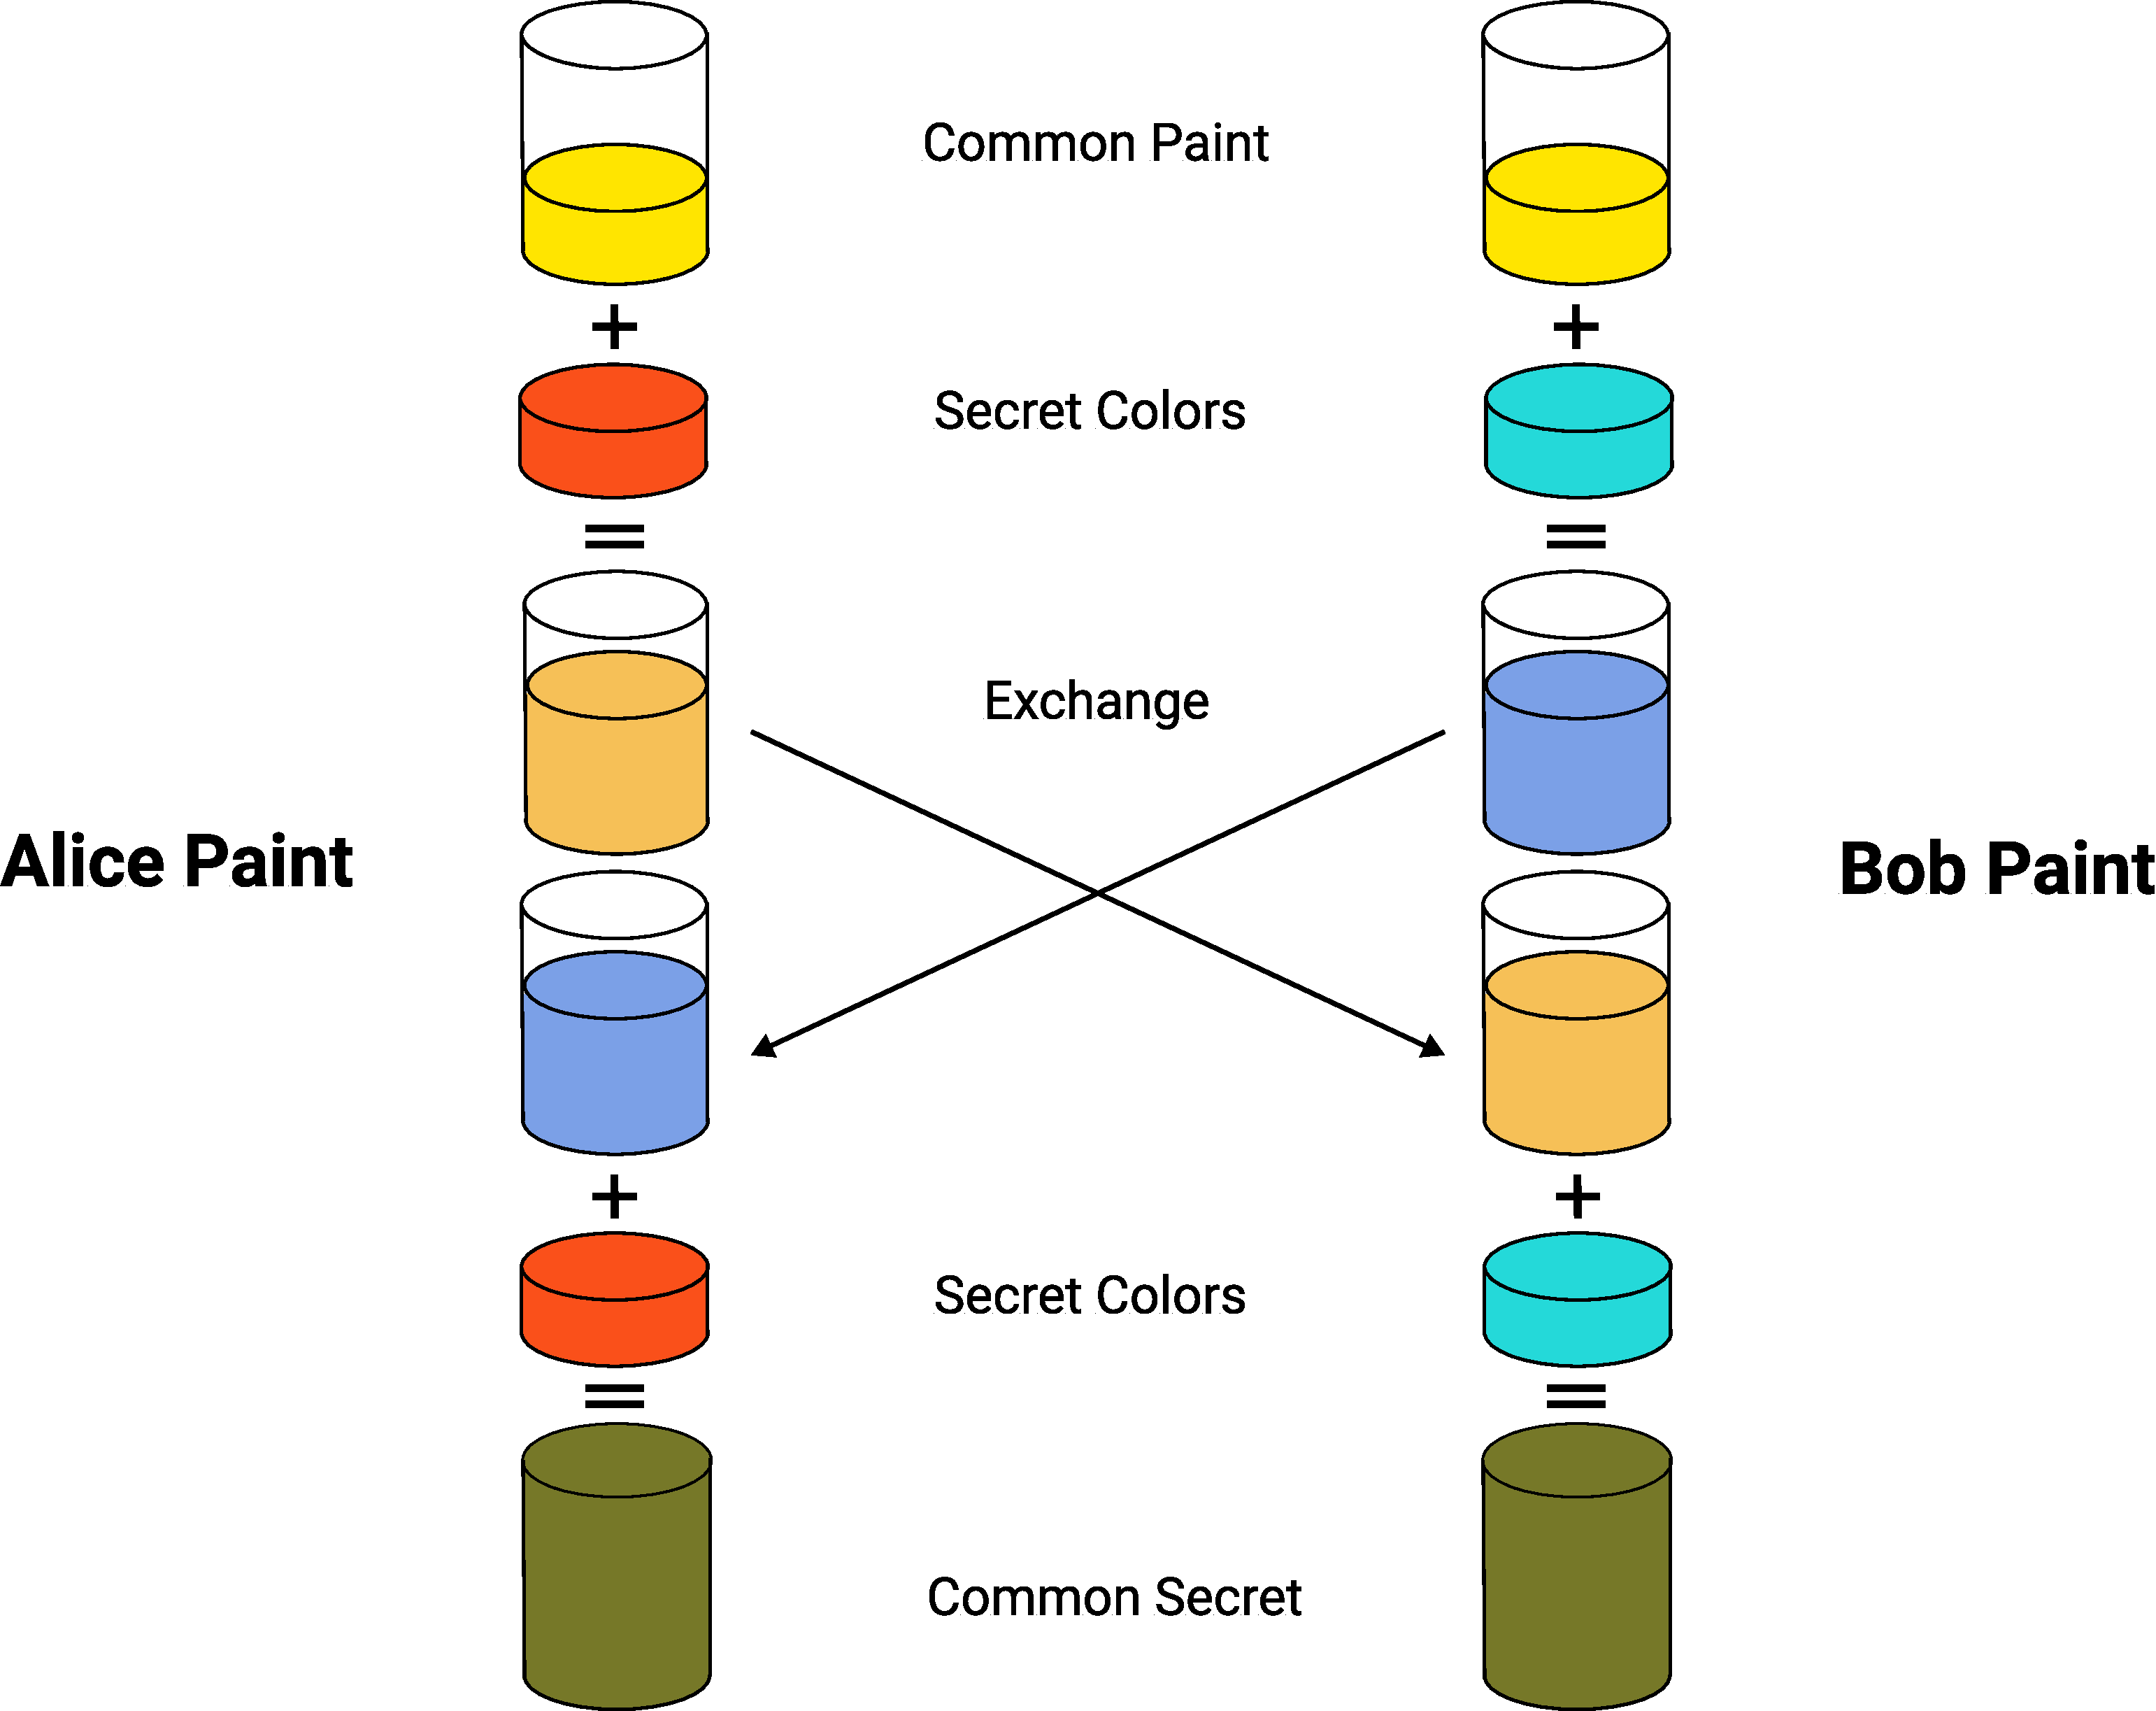
\includegraphics[width=1\textwidth]{Pictures/Diffie-Hellman}
    \caption{Illustration of the concept behind Diffie–Hellman key exchange. Source: }\label{fig:figure4}
\end{figure}
The process begins by having the two parties, Alice and Bob, publicly agree on an arbitrary starting color that does
not need to be kept secret (but should be different every time).
In this example, the color is yellow.
Each person also selects a secret color that they keep to themselves – in this case, red and blue-green.
The crucial part of the process is that Alice and Bob each mix their own secret color together with their mutually
shared color, resulting in orange-tan and light-blue mixtures respectively, and then publicly exchange the two mixed colors.
Finally, each of them mixes the color they received from the partner with their own private color.
The result is a final color mixture (yellow-brown in this case) that is identical to the partner's final color mixture.
If a third party listened to the exchange, it would only know the common color (yellow) and the first mixed colors
(orange-tan and light-blue), but it would be difficult for this party to determine the final secret color (yellow-brown).
Bringing the analogy back to a real-life exchange using large numbers rather than colors, this determination is
computationally expensive.
It is impossible to compute in a practical amount of time even for modern supercomputers.

The simplest and the original implementation of the protocol uses the multiplicative group of integers modulo $P$,
where $P$ is prime, and the generator $G$ which is a primitive root modulo $P$.
These two values are chosen in this way to ensure that the resulting shared secret can take on any value from $1$ to $P-1$.
Here is an example of the protocol
\begin{enumerate}
    \item Given modulus $P$ and generator $G$.
    \item Alice chooses her secret $a$.
    \item Alice sends to Bob $A, \; A = G^a \bmod P$.
    \item Bob chooses his secret $b$.
    \item Bob sends to Alice $B, \; B = G^b \bmod P$.
    \item Alice computes common secret $s, \; s = B^a \bmod P = (G^b \bmod P)^a \bmod P$.
    \item Bob computes common secret $s, \; s = A^b \bmod P = (G^a \bmod P)^b \bmod P$.
    \item Alice and Bob have arrived to the same value
    \[
        A^b \bmod P = G^{ab} \bmod P = G^{ba} \bmod P = B^a \bmod P,
    \]
    more specially,
    \[
        (G^a \bmod P)^b \bmod P = (G^b \bmod P)^a
    \]
\end{enumerate}
However, to reach a satisfactory level of security through DH key exchange a few rules have to be satisfied.
More precisely, Diffie-Hellman works in a multiplicative subgroup of integers modulo a given prime $p$.
To do some DH, you use some DH parameters which are:
\begin{itemize}
    \item p -- a big prime, called the "modulus"
    \item q -- a divisor of $p-1$, called the "subgroup order".
    \item g -- an integer modulo $p$ of order $q$, this means that the smallest integer $k > 0$ such that
    $g^k = 1 \bmod p$ is $k = q$.
\end{itemize}
For DH to be safe, you need the following:

\begin{itemize}
    \item Prime $p$ must defeat attempt at discrete logarithm through Index Calculus.
    This means that $p$ must be large enough, and also must not have any "special structure"
    such as being very close to a power of 2, because such structures allow for improvements in Index Calculus.
    It so happens that size requirements for DH are about the same as the size requirements for RSA,
    though the underlying reason for that is intricate and partly coincidental.
    So, basically, use a random $p$ of 2048 bits, and you will be fine.
    \item Number $q$ should be prime or have a prime divisor whose size is enough to defeat generic algorithms for
    discrete logarithm.
    If the size (in bits) of the largest prime divisor of $q$ is $z$, then generic algorithms have a cost in $2^{z/2}$.
    For best results, arrange for $q$ to be a prime of 256 bits or more.
    \item Systems that use the parameters to perform a DH key exchange must generate a random integer
    between $1$ and $q-1$ uniformly, using a cryptographically strong source of randomness, of course.
    If $q$ is prime and larger than 256 bits, it suffices to choose a 256-bit random value
    to achieve 128-bit of security.
    However, if $q$ is not prime, things are more complex: if $q$ has size $r$ bits,
    and the largest prime divisor of $q$ has size $e$ bits, and $e \geq 256$,
    then one may choose a random value $x$ of size $r-(e-256)$
    bits to get the usual "128-bit security".
    \item When $p$ is a so-called "safe prime", then $p = 2r+1$ for a prime $r$, so for any generator $g$ that is
    not $1$ or $p-1$, the order of $g$ will be either $r$ or $2r$, so it suffices to generate DH secret keys
    $x$ as random 257-bit values.
    The "safe primes" are not actually any safer than other primes,
    except for that point: they tolerate the choice of relatively small DH secret keys for any generator.
    \item Last but not least, DH is a key exchange algorithm that does not,
    inherently, provide authentication or confidentiality.
    DH is "safe" only when used within a protocol that uses DH and other algorithms with proper
    integration to achieve such sought after characteristics as data confidentiality and integrity.
\end{itemize}

Speaking of which, some (many) SSL/TLS implementations did things improperly, in that they
gladly accepted to do DH with weak parameters, in particular a 512-bit modulus.
The protocol itself is suboptimal in its handling of DH because the \texttt{ServerKeyExchange}
message allows the server to send the DH parameters $p$ and $g$ to the client, but not $q$,
leaving the client a bit in the dark.
Thus, the client must either "play safe" and generate its key in the full $1, \;\dots,\; p-1$ range,
or try to use a shorter exponent (say, 256 bits, not 2048) for a reduced computational cost,
but possibly at risk of weakness in case the subgroup order $q$ is not prime.
A better design would have allowed the server to send the value of $q$ and the size of the
biggest prime divisor of $q$.
In that respect, the ECDHE cipher suites of SSL/TLS (DH translated to elliptic curves)
have a better design.

For a practical answer if you are configuring your SSL/TLS server:
you should use a modulus of at least 2048-bit, and a generator $g$ such that the order
of $g$ is a prime $q$ of at least 256 bits;
alternatively, you may use a modulus $p$ which
is a "safe prime", the order of $g$ will then be either a very big prime, or twice
a very big prime, which is almost as good.
Some people feel safer when they generate their DH parameters
"themselves" instead of reusing existing values;
if that's what it takes
to allow you to sleep at night, then do it.

%\subsection{Secrecy Chart}\label{subsec:secrecy-chart}
%The chart below depicts who knows what, again with non-secret values in \textcolor{blue}{blue}, and secret values in \textcolor{red}{red}.
%Here Eve is an eavesdropper – she watches what is sent between Alice and Bob, but she does not alter the contents of their communications.
%\begin{itemize}
%    \item \textcolor{blue}{g} = public (prime) base, known to Alice, Bob, and Eve. $\textcolor{blue}{g = 5}$
%    \item \textcolor{blue}{p} = public (prime) modulus, known to Alice, Bob, and Eve. $\textcolor{blue}{p = 23}$
%    \item \textcolor{red}{a} = Alice's private key, known only to Alice. $\textcolor{red}{a = 6}$
%    \item \textcolor{red}{b} = Bob's private key known only to Bob. $\textcolor{red}{b = 15}$
%    \item \textcolor{blue}{A} = Alice's public key, known to Alice, Bob, and Eve. $\textcolor{blue}{A = g}^{\textcolor{red}{a}} \, mod \, \textcolor{blue}{p = 8}$
%    \item \textcolor{blue}{B} = Bob's public key, known to Alice, Bob, and Eve. $\textcolor{blue}{B = g}^{\textcolor{red}{a}} \, mod \, \textcolor{blue}{p = 8}$
%\end{itemize}
%\begin{center}
%    \begin{table}
%        \begin{tabular}{|c|c|c|c|c|c|}
%            \hline
%            \multicolumn{2}{|c|}{Alice} & \multicolumn{2}{c|}{Bob} & \multicolumn{2}{c|}{Eve}
%            \cr \hline
%            known & unknown & known & unknown & known & unknown
%            \cr \hline
%            $\textcolor{blue}{p = 23}$ & & $\textcolor{blue}{p = 23}$  & & $\textcolor{blue}{p = 23}$ &
%            \cr \hline
%            $\textcolor{blue}{g = 5}$ & & $\textcolor{blue}{g = 5}$ & & $\textcolor{blue}{g = 5}$ &
%            \cr \hline
%            $\textcolor{red}{a = 6}$ & $\textcolor{red}{b}$ & $\textcolor{red}{b = 15}$ & $\textcolor{red}{a}$ & & $\textcolor{red}{a, b}$
%            \cr \hline
%            $\textcolor{blue}{A = 5}^{\textcolor{red}{a}} \, mod \, \textcolor{blue}{23}$ & & $\textcolor{blue}{B = 5}^{\textcolor{red}{b}} \, mod \, \textcolor{blue}{23}$ & & &
%            \cr \hline
%            $\textcolor{blue}{A = 5}^{\textcolor{red}{6}} \, mod \, \textcolor{blue}{23} = \textcolor{blue}{8}$ & & $\textcolor{blue}{B = 5}^{\textcolor{red}{15}} \, mod \, \textcolor{blue}{23} = \textcolor{blue}{19}$ & & &
%            \cr \hline
%            $\textbf{\textcolor{blue}{B}} = \textbf{\textcolor{blue}{19}}$ & & $\textbf{\textcolor{blue}{A}} = \textbf{\textcolor{blue}{8}}$ & & $\textcolor{blue}{A} = \textcolor{blue}{8}$, $\textcolor{blue}{B} = \textcolor{blue}{19}$ &
%            \cr \hline
%            $\textbf{\textcolor{red}{s}} = \textcolor{blue}{B}^{\textcolor{red}{a}} \, mod \, \textcolor{blue}{23}$ & & $\textbf{\textcolor{red}{s}} = \textcolor{blue}{A}^{\textcolor{red}{b}} \, mod \, \textcolor{blue}{23}$ & & &
%            \cr \hline
%            $\textbf{\textcolor{red}{s}} = \textcolor{blue}{19}^{\textcolor{red}{6}} \, mod \, \textcolor{blue}{23} = \textcolor{red}{2}$ & & $\textbf{\textcolor{red}{s}} = \textcolor{blue}{A}^{\textcolor{red}{b}} \, mod \, \textcolor{blue}{23} = \textcolor{red}{2}$ & & &
%            \cr \hline
%
%        \end{tabular}
%        \label{tab:table}
%    \end{table}
%\end{center}
%Now \textcolor{red}{s} is the shared secret key and it is known to both Alice and Bob, but not to Eve.
%Note that it is not helpful for Eve to compute \textcolor{blue}{AB}, which equals
%$\textcolor{blue}{g}^{\textcolor{red}{a} + \textcolor{red}{b}} \, mod \, \textcolor{blue}{p}$.
%Note that it should be difficult for Alice to solve for Bob's private key or for Bob to solve for Alice's private key.
%If it is not difficult for Alice to solve for Bob's private key (or vice versa), Eve may simply substitute her own
%private / public key pair, plug Bob's public key into her private key, produce a fake shared secret key, and solve for
%Bob's private key (and use that to solve for the shared secret key.
%Eve may attempt to choose a public / private key pair that will make it easy for her to solve for Bob's private key).

\begin{figure}[H]
    \centering
    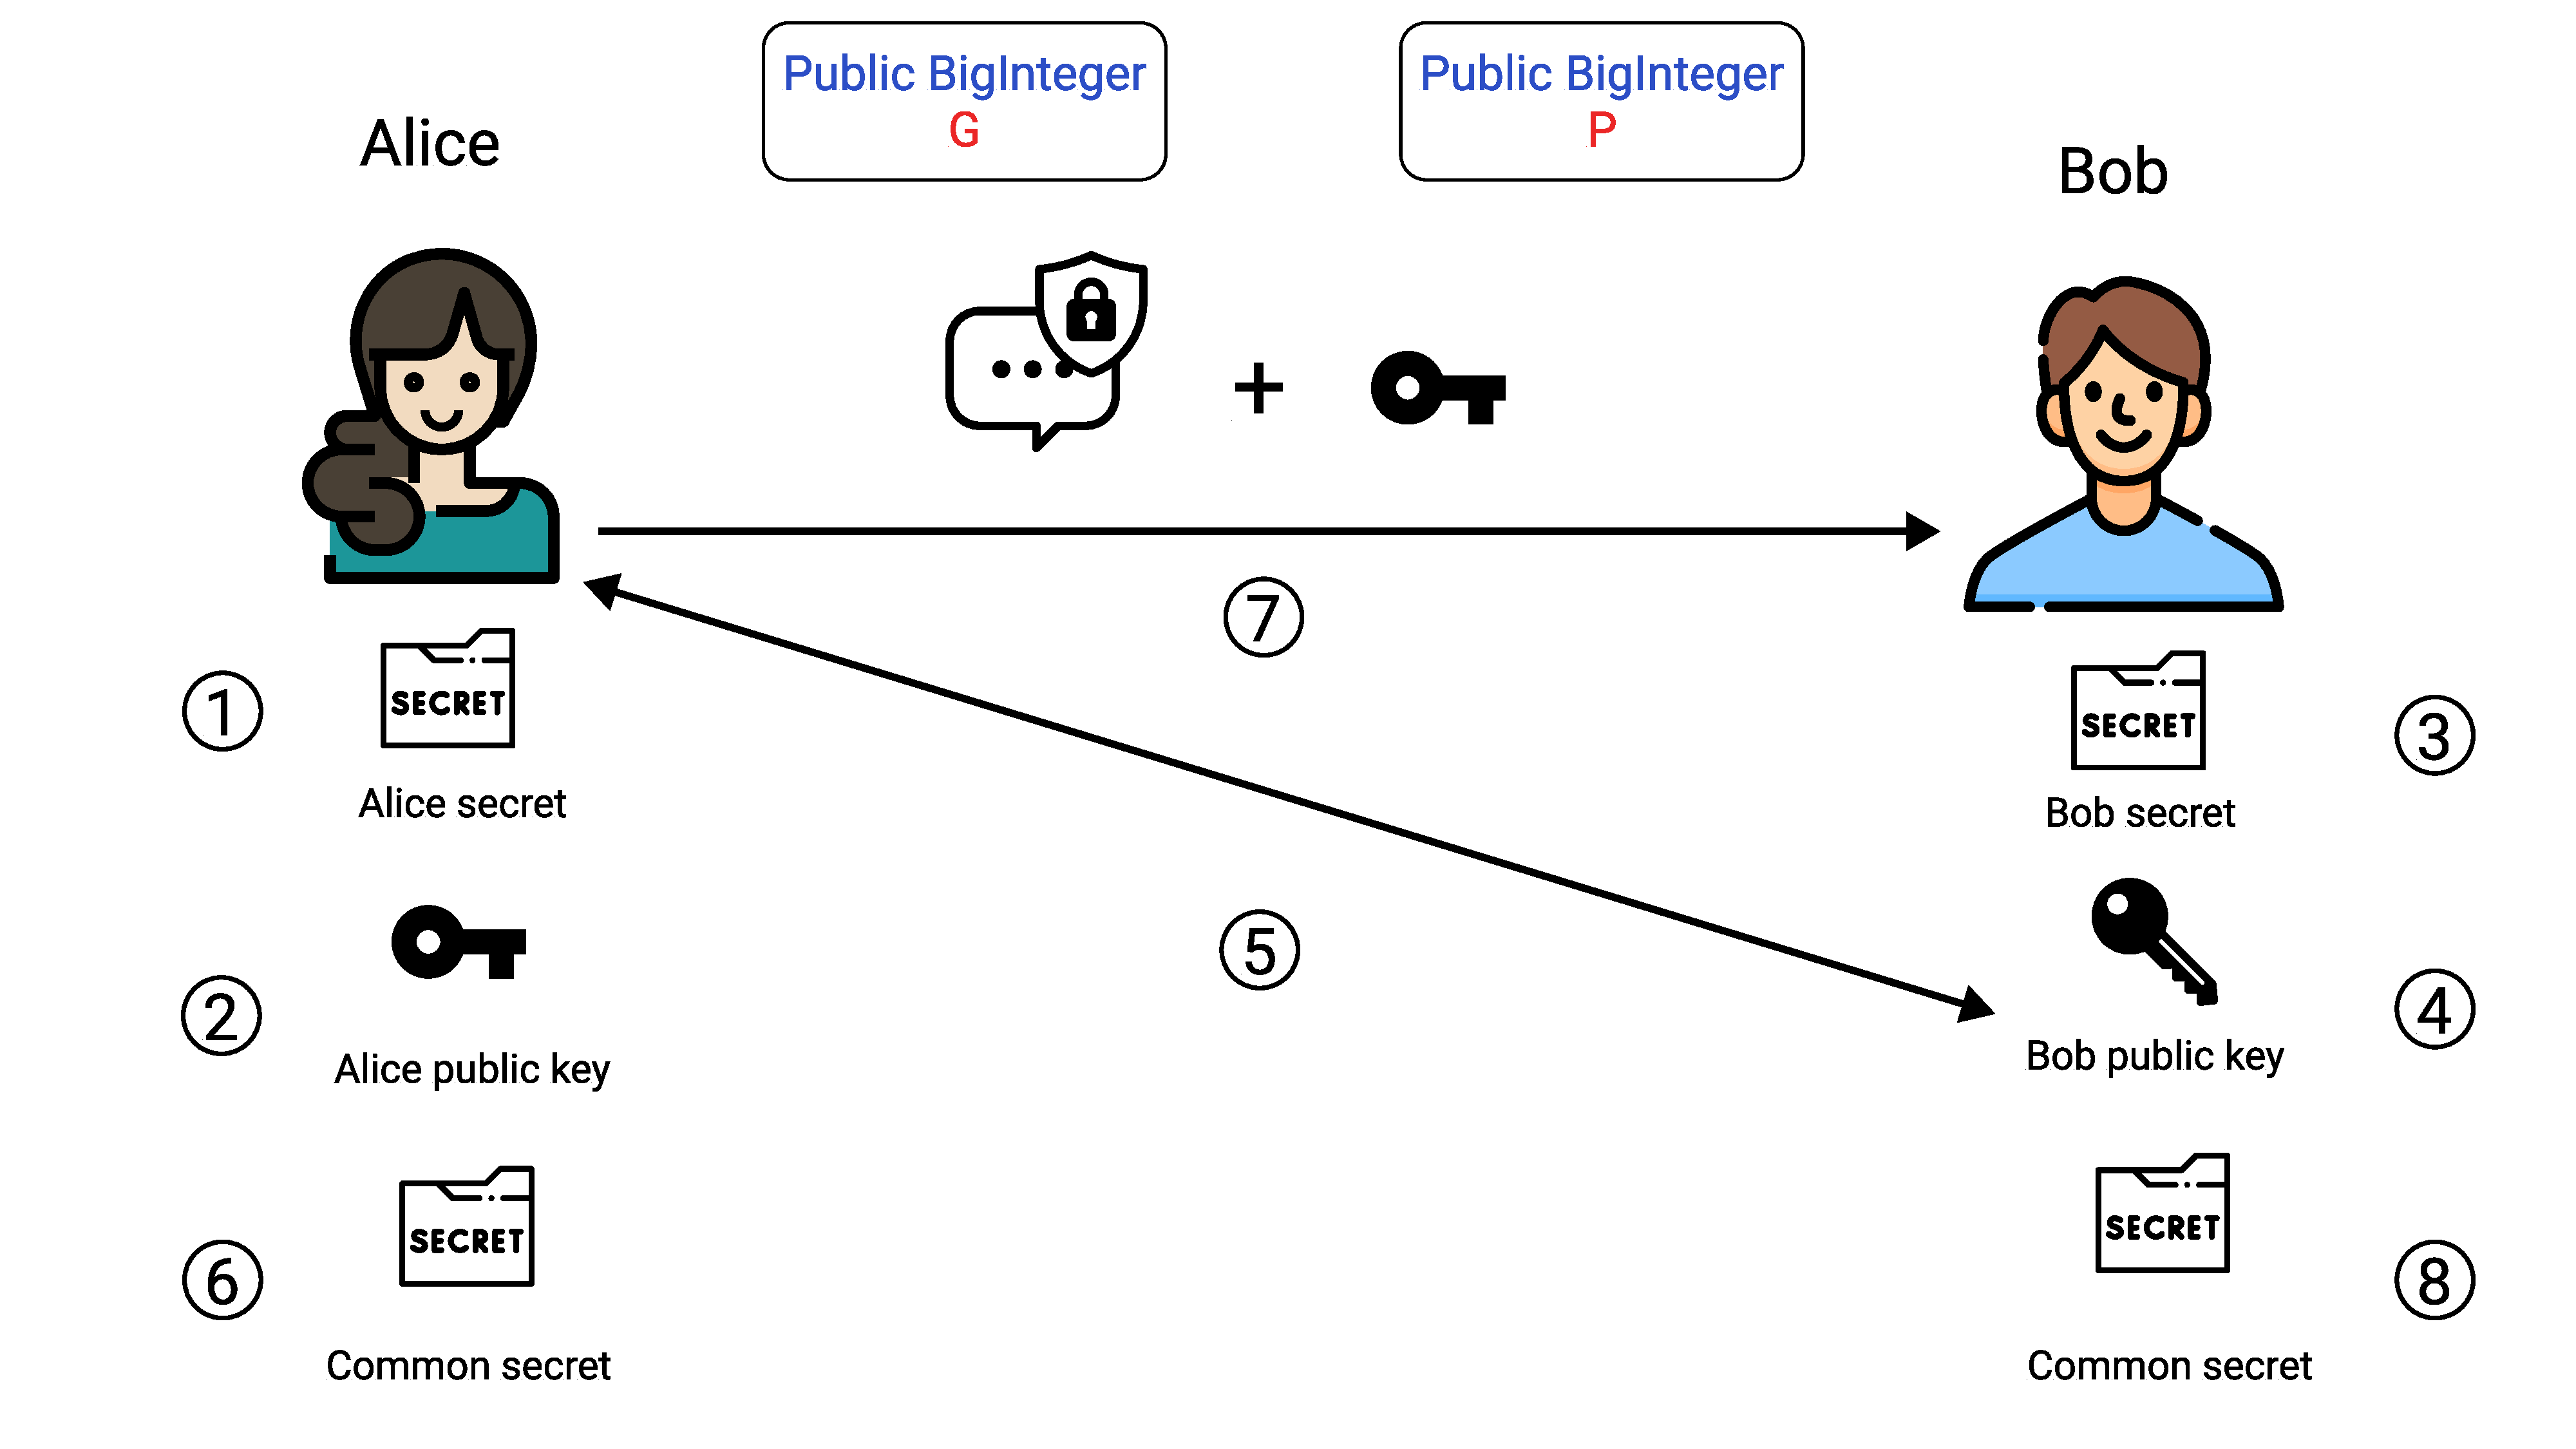
\includegraphics[width=1\textwidth]{Pictures/Key_Exchange}
    \caption{Secret chat encryption concept diagram. Source: }\label{fig:figure7}
\end{figure}
Assume that Alice wants to write a secret message to the Bob.
The secret chat encryption implemented as follows
\begin{enumerate}
    \item Given two public constants: $P, G$.
    \item Alice generates her secret $a$.
    \item Alice generates public key $A$ as $A=G^a \bmod P$ and shares it public.
    \item Bob generates his secret $b$.
    \item Bob generates public key $B$ as $B=G^b \bmod P$ and shares it public.
    \item Alice reads Bob's public key $B$.
    \item Alice calculates Common secret $s$ as $s = B^a \bmod P$.
    \item Alice encrypts message using AES256 algorithm, then sends it to Bob along her public key $A$.
    \item Bob calculates Common secret $s$ as $s = A^b \bmod P$ and decrypts message from Alice.
\end{enumerate}
Although, DH fits the key exchange concerns fine, the secret might be shared via RSA approach as well.
We discuss it in next section.
%    \chapter{Architectural aspects of the system}\label{ch:architectural-aspects-of-the-system}


\section{Application architecture and related comments}\label{sec:application-architecture-and-related-comments}
As a programmers, I believe all we have faced the cases of crucial over-engineering during the implementation of some
software product.
For the programmer, it is a vital point to follow two separated, but closely related software development principles,
such that KISS [\cite{alwin2016kiss}], and YAGNI [\cite{da2018evolution}].
As the main topic of our thesis is to implement Instant Messaging System following the security and privacy aspects.
We consider to following above-mentioned development principles KISS and YAGNI and approach
a well-known N-tier application Monolithic architecture [\cite{bucchiarone2018monolithic}], which provides a model by which developers can
create flexible and reusable applications.
By segregating an application into tiers, developers acquire the option of modifying or adding a specific layer,
instead of reworking the entire application.
A three-tier architecture is typically composed of a presentation tier, a logic tier, and a data tier.
One would suggest to use nowadays popular Microservices Architecture, thinking about scalability [\cite{brataas2004exploring}],
an ability of the system to handle large numbers of users distributed over geographically large areas without
notably affecting the overall performance of the system.
However, the effect of Microservices is being felt only for quite large and complex systems,
not the case of our yet simple application.
Following plot demonstrates this relation

\begin{figure}[H]
    \centering
    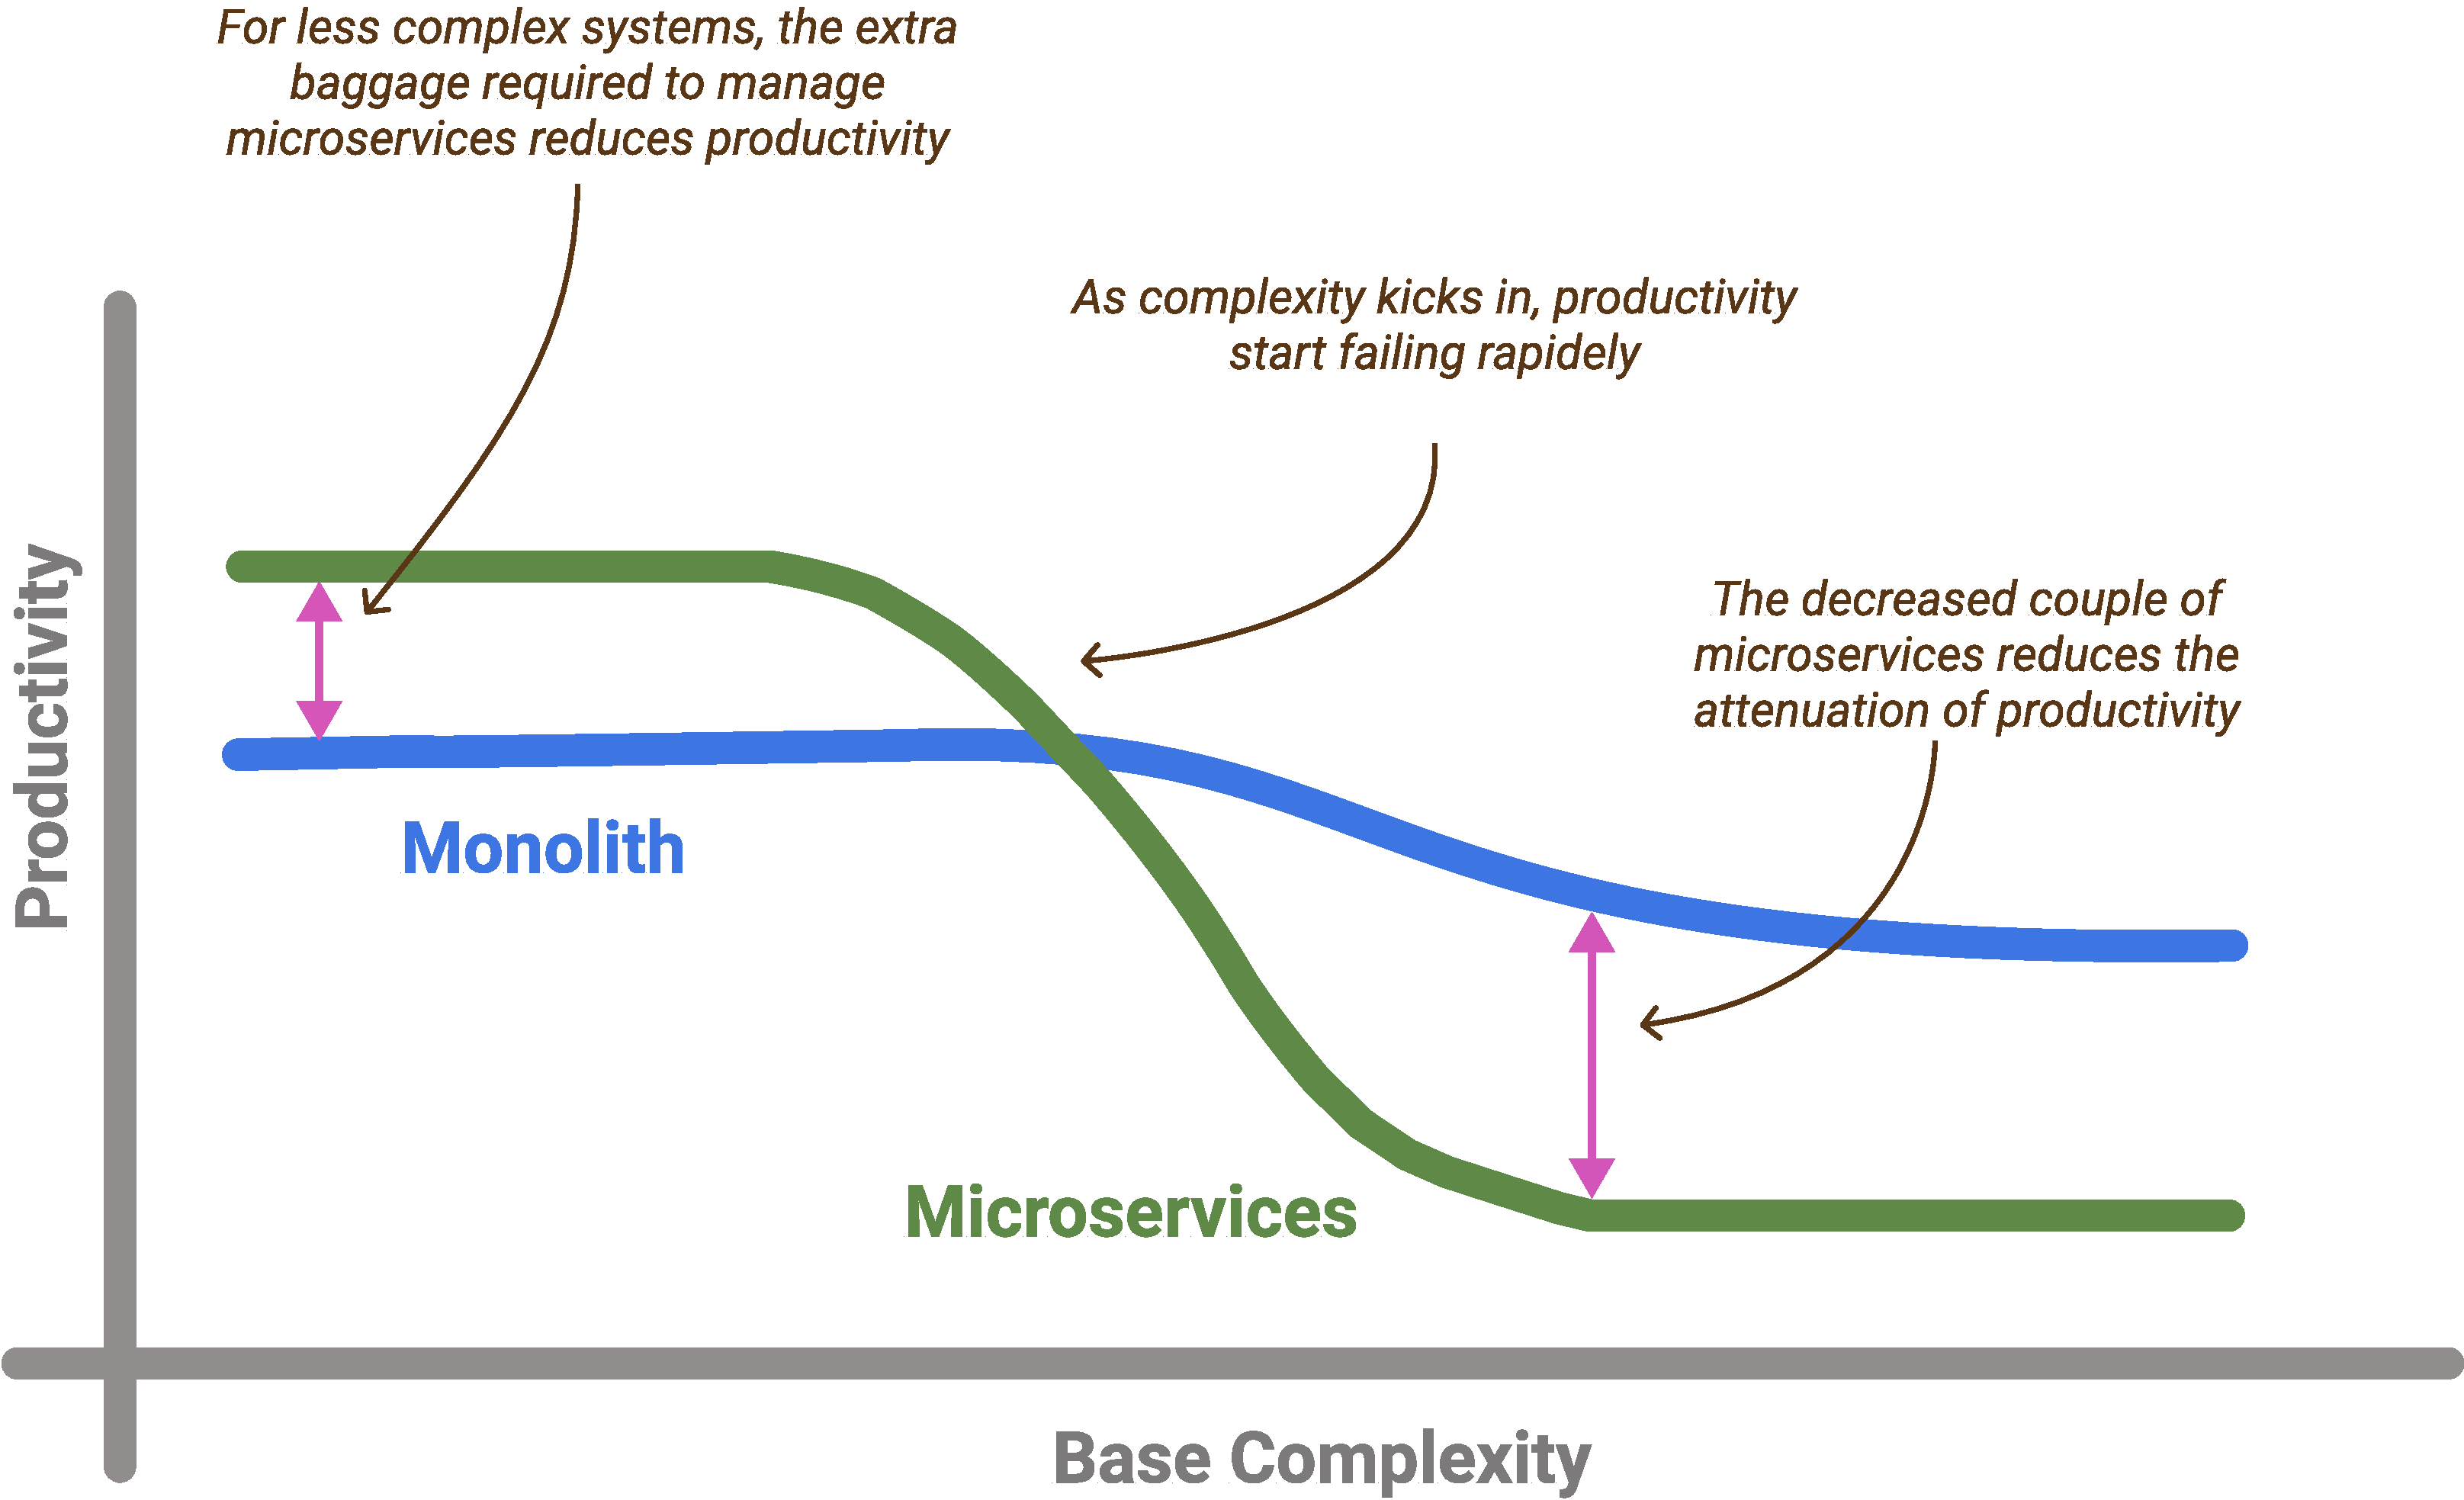
\includegraphics[width=1\textwidth]{Pictures/Monolith_vs_Microservice.pdf}
    \caption{Relation between system complexity and architectures. Source: https://martinfowler.com/bliki/MicroservicePremium.html}
    \label{fig:monolith_vs_microservice}
\end{figure}

In a logical multilayer architecture for an information system with an object-oriented design, the following four are the most common:

\begin{itemize} % source: https://en.wikipedia.org/wiki/Multitier_architecture#cite_note-5
    \item \textbf{Presentation Layer.} UI layer, view layer, presentation tier in multitier architecture.
    \item \textbf{Application Logic.} Service layer [\cite{ji2009intelligent, swetina2014toward}]
    or GRASP Controller Layer [\cite{okada2006vision}].
    \item \textbf{Business Logic.} Business logic layer, domain logic layer.
    \item \textbf{Data Access Layer.} Persistence layer, logging, networking, and other services which are required
    to support a particular business layer.
\end{itemize}

\begin{figure}[H]
    \centering
    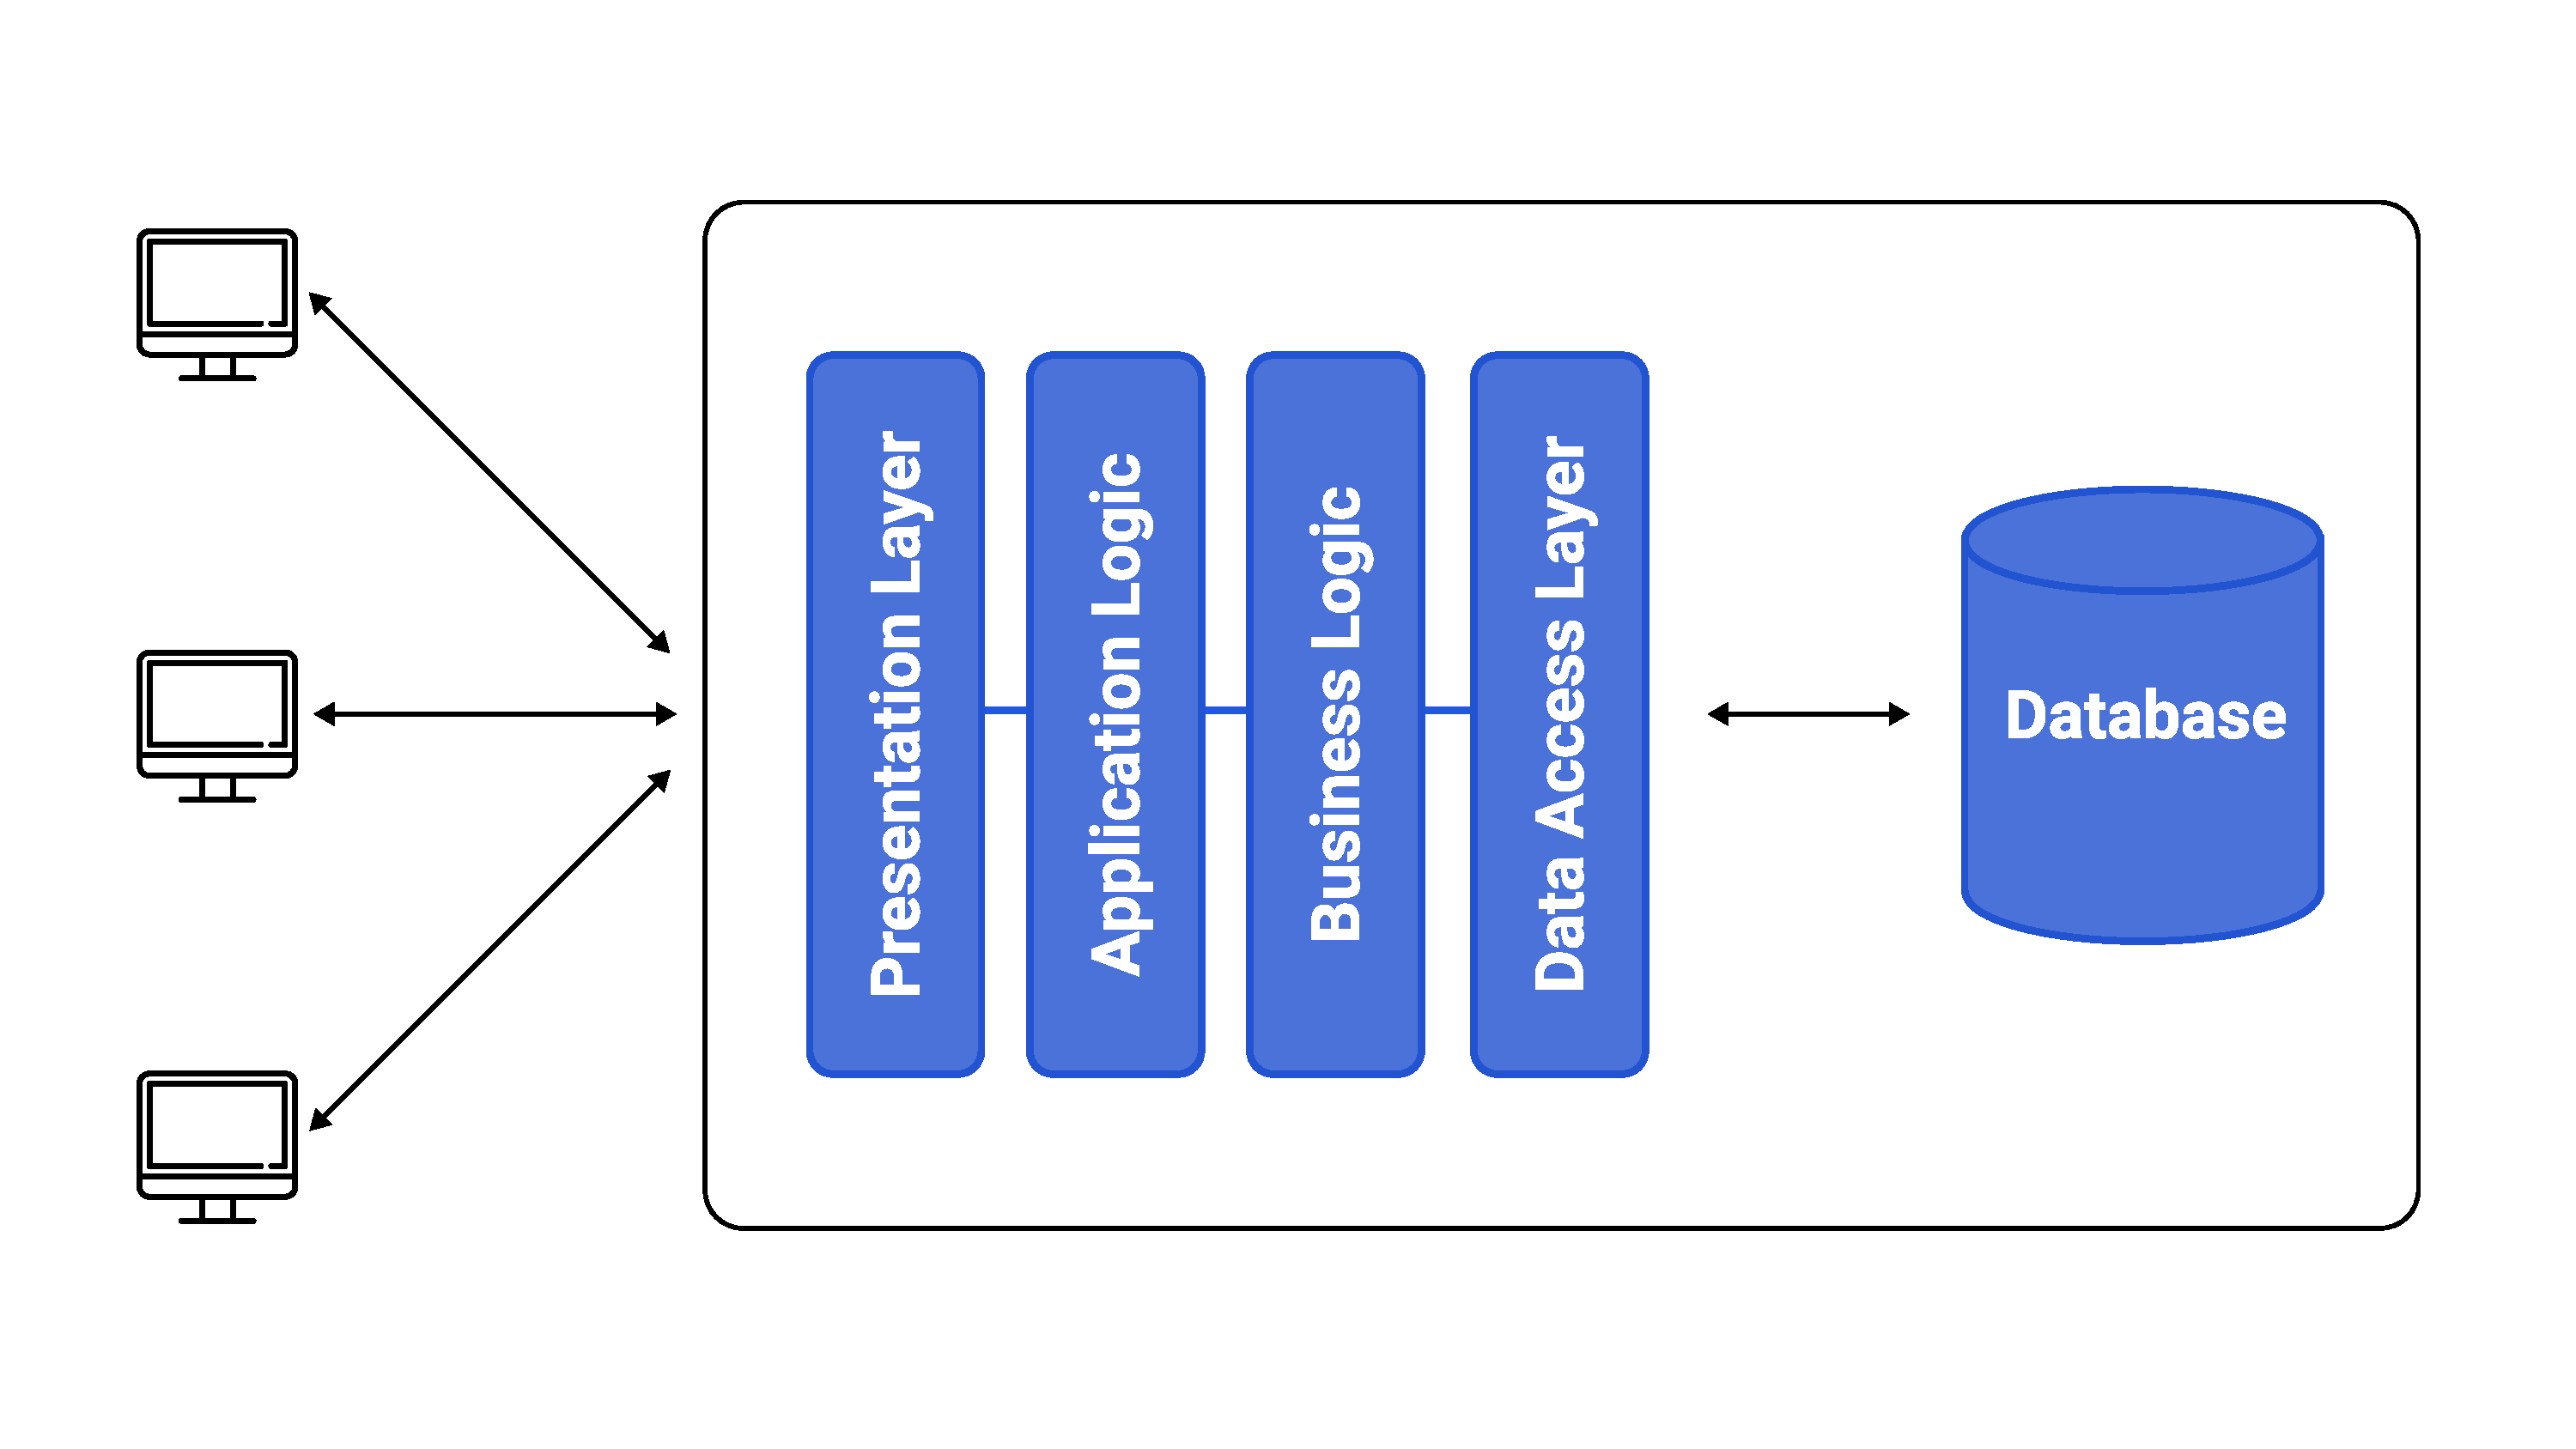
\includegraphics[width=1\textwidth]{Pictures/Monolith_architecture.pdf}
    \caption{Monolithic architecture diagram. Source: }\label{fig:figure2}
\end{figure}

The book Domain Driven Design describes some common uses for the above four layers, although its primary focus is the
domain layer [\cite{solvberg2010domain}].
If the application architecture has no explicit distinction between the business layer and the presentation layer,
then a traditional client-server model has been implemented.
The presentation layer is considered part of the business layer.
The more usual convention is that the application layer is considered a sublayer of the business layer,
typically encapsulating the API definition surfacing the supported business functionality.
The application/business layers can, in fact, be further subdivided to emphasize additional sub-layers of distinct
responsibility.
For example, if the model–view–presenter pattern is used, the presenter sublayer might be used as an additional layer
between the user interface layer and the business/application layer, as represented by the model sublayer.
Some also identify a separate layer called the business infrastructure layer, located between the business layer
and the infrastructure layer.
It's also sometimes called the \textit{low-level business layer} or the \textit{business services layer}.
The infrastructure layer can be partitioned into different levels, high-level or low-level technical services [\cite{dennis2018mcapl}].
Developers often focus on the persistence capabilities of the infrastructure layer and therefore only
talk about the persistence layer or the data access layer instead of an infrastructure layer or technical services layer.
In other words, the other kind of technical services are not always explicitly thought of as part of any particular layer.
A layer is on top of another, because it depends on it.
Every layer can exist without the layers above it, and requires the layers below it to function.
Another common view is that layers do not always strictly depend on only the adjacent layer below.
For example, in a relaxed layered system, a layer can also depend on all the layers below it [\cite{anon2014building}].
Relaxed layered system may be considered as opposed to a strict layered system.

\subsection{Monolith Architecture: Cons and Props}\label{subsec:monolith-architecture:-cons-and-props}

A monolith is built as a large system with a single code base and deployed as a single unit, usually behind a load balancer.
It typically consists of four major components: a user interface, business logic, a data interface and a database.
Monoliths offer several advantages, particularly when it comes to operational overhead requirements.
Here are some of those basic benefits:

\begin{itemize}
    \item \textbf{Simplicity.} Monolithic architectures are simple to build, test and deploy.
    These apps can scale horizontally, in one direction, by running several copies of the application behind a load balancer.
    Cross-cutting concerns: With a single codebase, monolithic apps can easily handle cross-cutting concerns, such as logging,
    configuration management and performance monitoring.
    Another advantage associated with the simplicity of monolithic apps is easier deployment.
    When it comes to monolithic applications, you do not have to handle many deployments – just one file or directory.
    \item \textbf{Performance.} Components in a monolith typically share memory which is faster than service-to-service
    communications using IPC [\cite{proctor1999linux}] or other mechanisms.
    \item \textbf{Easier debugging and testing.}
    In contrast to the microservices architecture, monolithic applications are much easier to debug and test.
    Since a monolithic app is a single indivisible unit, you can run end-to-end testing much faster.
    \item \textbf{Easier development.} As long as the monolithic approach is a standard way of building applications,
    any engineering team has the right knowledge and capabilities to develop a monolithic application.
\end{itemize}
But one major drawback of monolithic architectures is tight coupling.
Over time, monolithic components become tightly coupled and entangled.
This coupling effects management, scalability and continuous deployment.
Other cons that stem from tight coupling include:
\begin{itemize}
    \item \textbf{Understanding.} When a monolithic application scales up, it becomes too complicated to understand.
    Also, a complex system of code within one application is hard to manage.
    \item \textbf{Reliability.} An error in any of the modules in the application can bring the entire application down.
    \item \textbf{Updates.} Due to a single large codebase and tight coupling, the entire application would have to deploy
    for each update.
    \item \textbf{Technology stack.} A monolithic application must use the same technology stack throughout.
    Changes to the technology stack are expensive, both in terms of the time and cost involved.
    \item \textbf{Scalability.} You cannot scale components independently, only the whole application.
\end{itemize}

\subsection{Decoupling Monolith using CQRS}\label{subsec:decoupling-monolith-using-cqrs}
As it stated in previous section, monolithic architecture provides a quite strong coupling between application
components.
Moreover, as monolith grow horizontally, its services layer grows as well.
This process leads to very huge code base which is very difficult to support and extend.
We attach the following
\href{https://github.com/smartstore/SmartStoreNET/blob/4.x/src/Presentation/SmartStore.Web/Controllers/CatalogHelper.cs}
{link}
as an example of such approach.
To avoid the natural results of monolithic architecture, that are huge classes for thousands lines, we have to dive into
design patterns [\cite{rising1998design}].
Precisely, the mediator design pattern would help to decouple the service layer from presentation layer.
Mediator -- is a behavioral design pattern [\cite{rasche2016building}] that lets you reduce chaotic dependencies between objects.
The pattern restricts direct communications between the objects and forces them to collaborate only via a mediator object.
In other words, mediator allows the communication between two entities, such that entities doesn't know each other.
The Mediator pattern suggests that you should cease all direct communication between the components which you want to make
independent of each other.
Instead, these components must collaborate indirectly, by calling a special mediator object that redirects the calls to
appropriate components.
As a result, the components depend only on a single mediator class instead of being coupled to dozens of their colleagues.
In context of .NET platform there are multiple implementation of the Mediator, the most widely known and used is the
\href{https://github.com/jbogard/MediatR}{MediatR}, which we use in our project.
Another, yet popular approach is the CQRS, which stands for Command-Query Responsibility Segregation.
In brief, it stands that read (query) and write (command) requests should be segregated by their responsibilities.
The CQRS approach in couple with Mediator greatly helps to solve the coupling problem of the monolith architecture.
So what is CQRS precisely?
According to \href{https://martinfowler.com/bliki/CQRS.html}{Martin Fowler},
it is a pattern that first described by Greg Young [\cite{young2010cqrs}].
At its heart is the notion that you can use a different model to update information than the model you use to read information.
For some situations, this separation can be valuable, but beware that for most systems CQRS adds risky complexity.
The mainstream approach people use for interacting with an information system is to treat it as a CRUD datastore.
By this meant that we have mental model of some record structure where we can create new records, read records,
update existing records, and delete records when we're done with them.
In the simplest case, our interactions are all about storing and retrieving these records.
As our needs become more sophisticated we steadily move away from that model.
We may want to look at the information in a different way to the record store, perhaps collapsing multiple records into one,
or forming virtual records by combining information for different places.
On the update side we may find validation rules that only allow certain combinations of data to be stored, or may even infer
data to be stored that's different from that we provide.
For instance, the idea of command-query segregation is displayed at the following image

\begin{figure}[H]
    \centering
    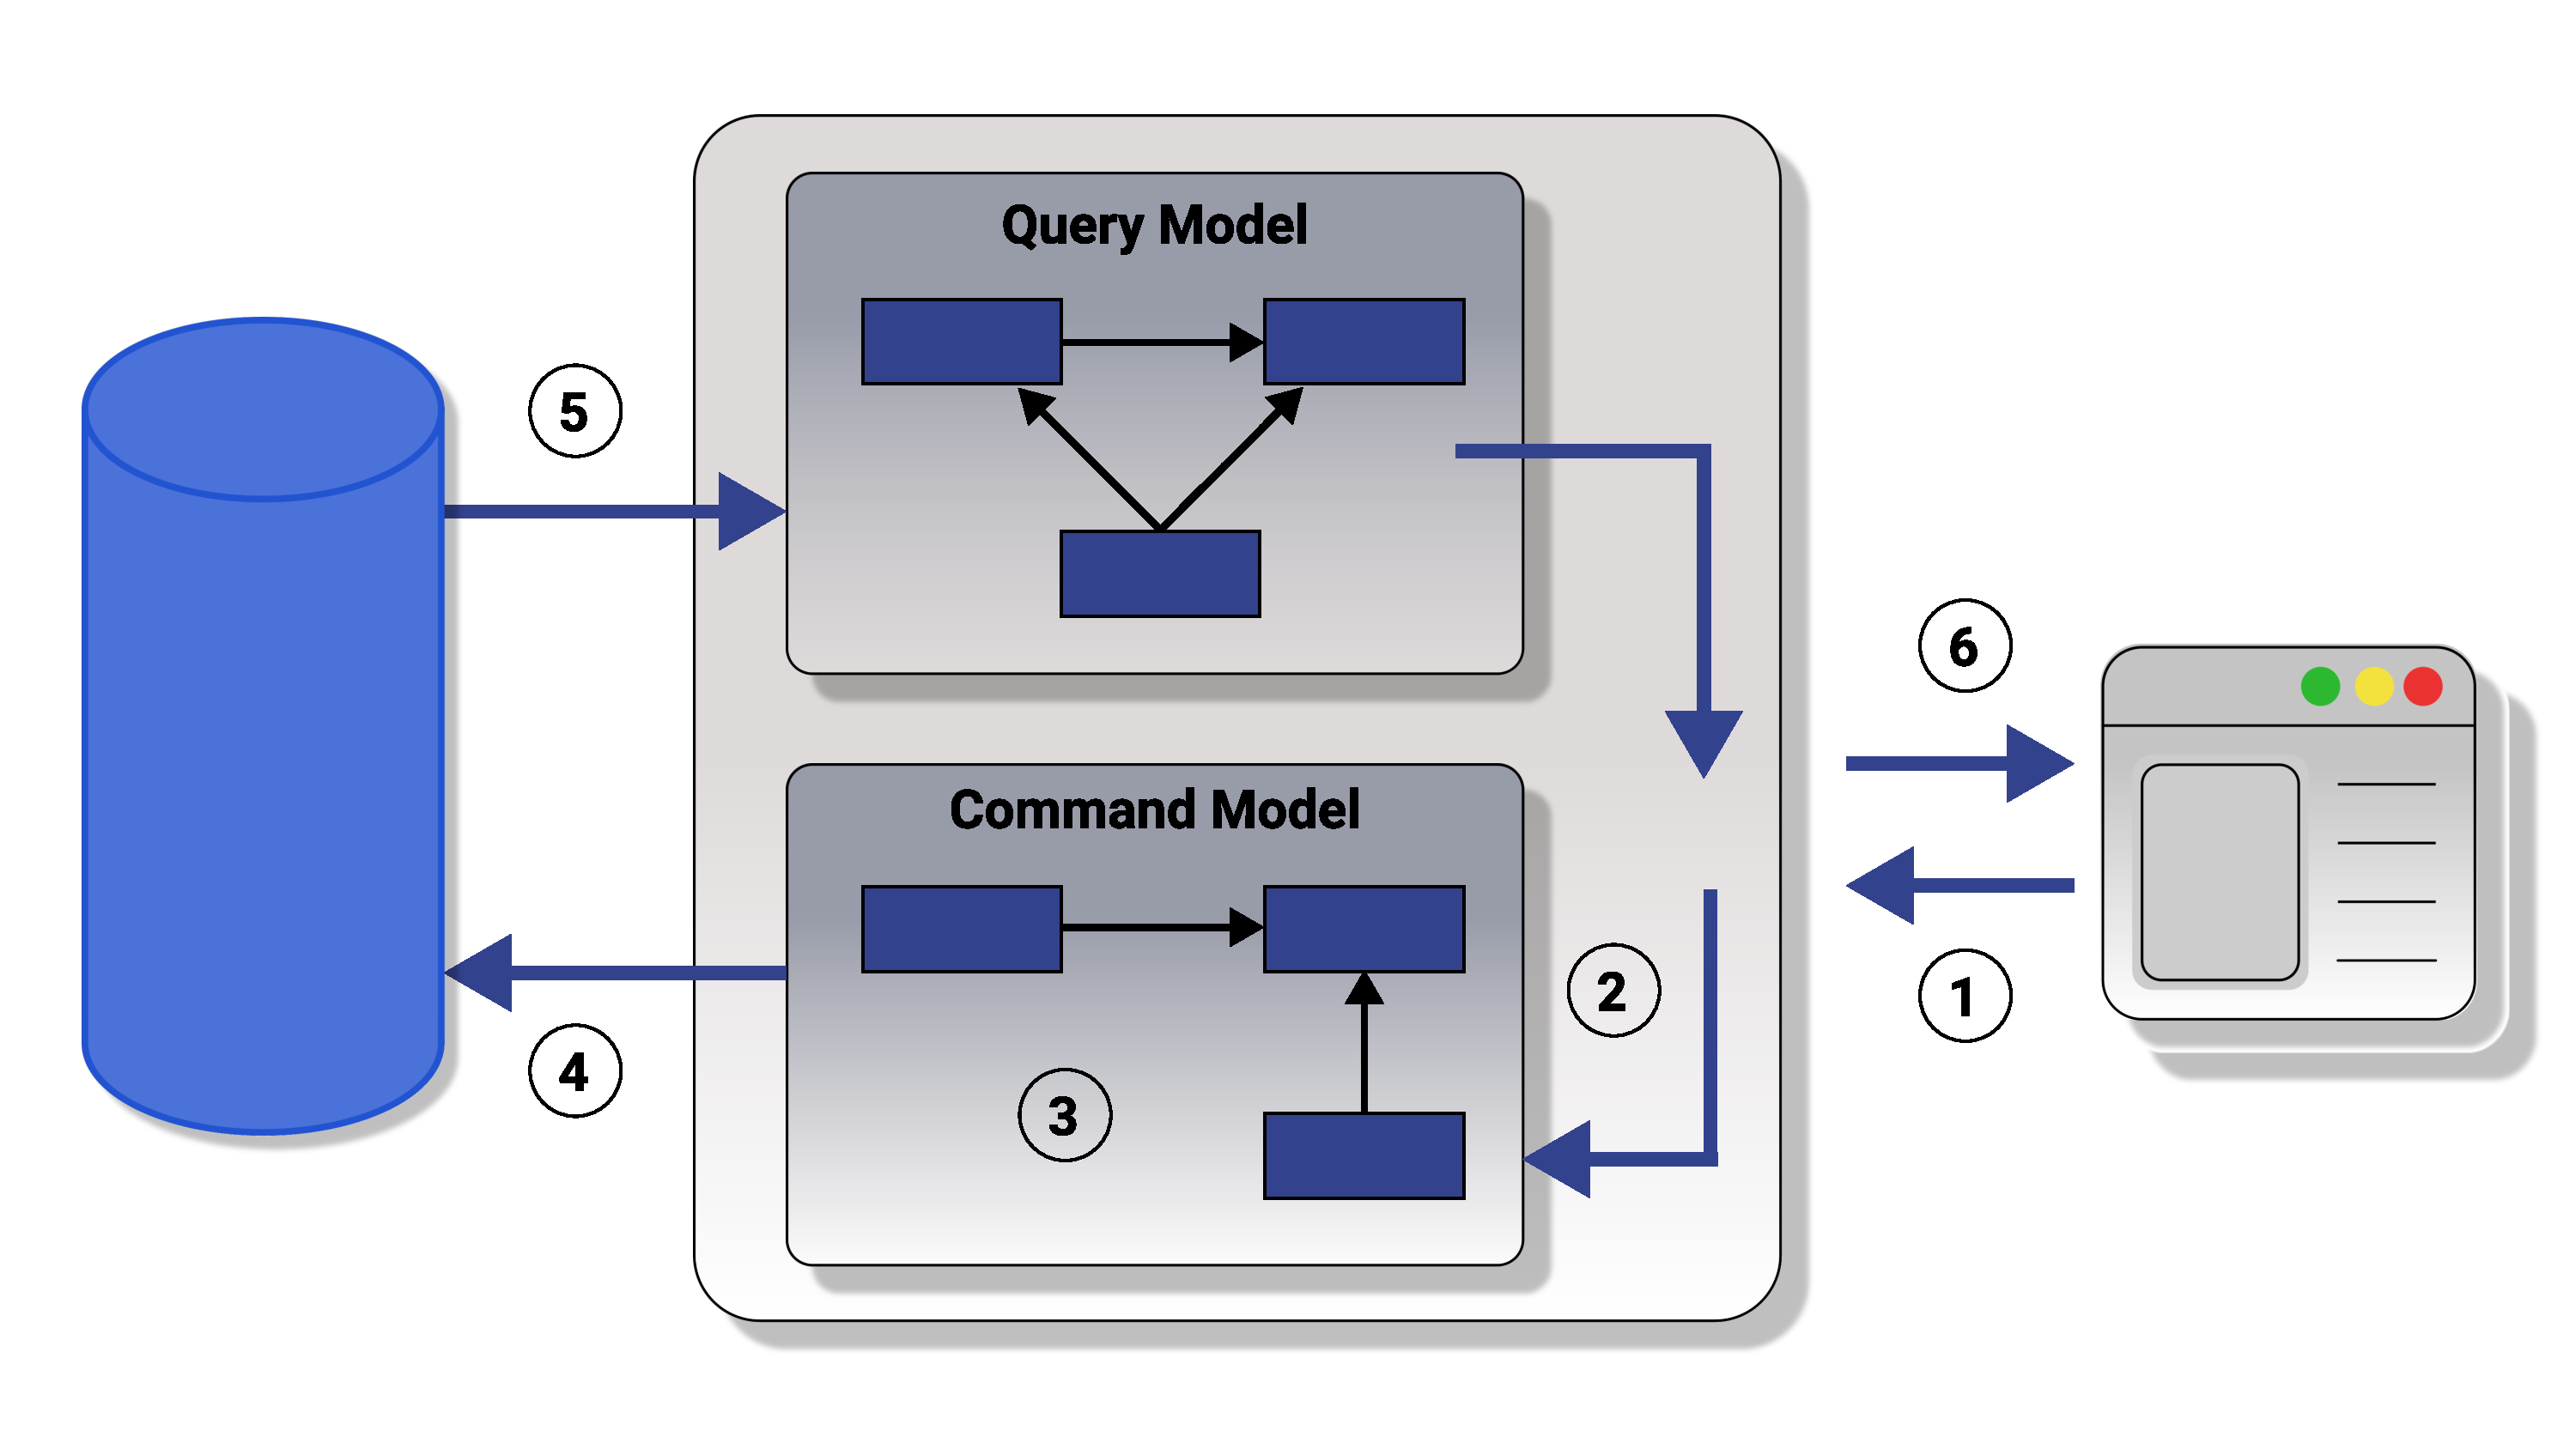
\includegraphics[width=1\textwidth]{Pictures/cqrs.pdf}
    \caption{CQRS Conceptual diagram. Source: https://martinfowler.com/bliki/CQRS.html}\label{fig:figure}
\end{figure}

\begin{enumerate}
    \item User makes a change in UI\@.
    \item Application routes information to command model.
    \item Command model executes validation and business logic.
    \item Command model updates the database.
    \item Query model reads from database.
    \item Query service update presentation from query model.
\end{enumerate}

Despite these benefits, you should be very cautious about using CQRS\@.
Many information systems fit well with the notion of an information base that is updated in the same way that it's read,
adding CQRS to such a system can add significant complexity.
I've certainly seen cases where it's made a significant drag on productivity, adding an unwarranted amount of risk to the
project, even in the hands of a capable team.
So while CQRS is a pattern that's good to have in the toolbox, beware that it is difficult to use well and you can easily
chop off important bits if you mishandle it.

As a short conclusion, we may state that CQRS and Mediator pattern will not entirely solve the coupling problems the monolith,
however will make project much more simplistic and intuitively understood.
It is worth to keep is simple,
even relatively simple project may grow to the sizes of universe without proper architectural solutions.

\subsection{Database Structure and related comments}\label{subsec:database-structure-and-related-comments}
As a next topic to uncover goes the one related to the database structure.
Proper database structure is to be of very high priority, since it influences on the project as a whole,
starting from performance point of view and many other aspects.
When we say performance, we mean such a design of database that there is an opportunity to include required indexes,
depending on regularity of any particular request.
So, as the main topic of current thesis is implementation of Instant messaging system, we can list the following
general entities to be added to database schema.

\begin{itemize}
    \item \textbf{Users.} Table stores information about user.
    Table contains following columns:
    \begin{itemize}
        \item Id VARCHAR(36) -- Id of the user, primary key, GUID\@.
        \item UserName VARCHAR(50) -- Unique Username.
        \item NormalizedUserName VARCHAR(50) -- Unique Username in upper case.
        \item DisplayName VARCHAR(50) -- Name of the user, displayed to others.
        \item Bio VARCHAR(250) -- User's short biography, visible to others.
        \item Image VARCHAR(36) -- User's profile picture, visible to others.
        \item Email VARCHAR(120) -- User's email address, not public.
        \item EmailConfirmed BOOLEAN -- Flag that indicates if user has confirmed his email address.
        \item PhoneNumber VARCHAR(50) -- User's phone number.
        \item PhoneNumberConfirmed BOOLEAN -- Flag that indicates if user has confirmed his phone number.
        \item PhoneVerificationCode INTEGER -- Code sent to user in order to confirm phone number.
        \item PasswordHash VARCHAR(60) -- Hashed password.
        \item CreatedAt DATETIME -- Indicates the date and time user has been registered.
        \item UpdatedAt DATETIME -- Indicates the date and time user has updated his record.
    \end{itemize}
    \item \textbf{User Personal Information.} Table stores additional but not required info about user.
    Relation one-to-one with Users, foreign key is UserId, GUID\@.
    Table contains following columns:
    \begin{itemize}
        \item UserId VARCHAR(36) -- Foreign key to the Users table, GUID\@.
        \item FirstName VARCHAR(120) -- First name of user.
        \item LastName VARCHAR(120) -- Last name of user.
        \item BirthDay DATETIME -- Birth day of user.
        \item WebSite VARCHAR(120) -- Web site of user.
        \item Address VARCHAR(120) -- Residence address of user.
        \item Facebook VARCHAR(120) -- Facebook nickname of user.
        \item Twitter VARCHAR(120) -- Twitter nickname of user.
        \item Instagram VARCHAR(120) -- Instagram nickname of user.
        \item LinkedIn VARCHAR(120) -- LinkedIn nickname of user.
        \item ProfilePicture VARCHAR(36) -- Avatar of user.
    \end{itemize}
    \item \textbf{UserContacts.} Table stores the contacts of current user.
    Relation between tables Users and UserContacts is one-to-many, foreign key UserId.
    Table contains following columns:
    \begin{itemize}
        \item ContactId VARCHAR(36) -- Id of current user's contact, GUID\@.
        \item UserId VARCHAR(36) -- Id of current user, GUID\@.
    \end{itemize}
    \item \textbf{Chats.} In order to communicate with other people it is essentially to have a chat room.
    Our implementation provides chat rooms of the four types.
    Direct chat -- chat room between only two members.
    Public channel -- chat room for multiple members, each member can send and read messages.\ It displayed in search results.
    Readonly channel -- channel for multiple members, however only the owner can send messages.\ It displayed in search results.
    Private channel -- channel for multiple members, can be joined only by invite link.
    Each user can have a numerous various chats, however, each chat has a multiple members, at least 2 as the case of direct chat.
    Therefore, we consider a many-to-many relation between user and chats via intermediate table UserChats.
    We discuss UserChats relation in foregoing part.
    Continuing with Chats table, it contains the following columns:
    \begin{itemize}
        \item Id VARCHAR(36) -- Id of the chat, primary key, GUID.
        \item ChatInfoId VARCHAR(36) -- Since we have a four types of channels, which has a common subset of data,
        the different data is moved to another table, so it could be joined depending on chat type.
        For instance, any chat type except direct one would require to join additional data in order to display the chat properly.
        \item Title VARCHAR(50) -- Simply, the title of the chat.
        \item Image VARCHAR(36) -- Picture of the chat.\ Displayed in search results etc.
        \item ChatType ENUM -- The type of the chat, e.g direct chat, public channel, readonly channel, private channel.
        \item CreatedAt DATETIME -- Indicates the date and time chat has been created.
        \item UpdatedAt DATETIME -- Indicates the date and time chat has been updated.
    \end{itemize}
    \item \textbf{UserChats.} Table that considered as composite key of the many-to-many relation between Users and Chats tables.
    Over that, contains an enum value that indicates user's role in the chat.
    We assume the following user roles in the system:
    \begin{itemize}
        \item Owner -- the creator of the chat.
        Has an ultimate privileges.
        \item Administrator -- designated by the owner user, which has adjustable privileges.
        \item Moderator -- designated by administrator user, which has adjustable privileges.
        \item User -- default role assigned to the user on join the chat.
    \end{itemize}
    Despite that, the UserChats table contains the following columns:
    \begin{itemize}
        \item ChatId VARCHAR(36) -- Foreign key to the Chats table, GUID\@.
        \item UserId VARCHAR(36) -- Foreign key to the Users table, GUID\@.
        \item RoleId ENUM -- Indicates the user role in the chat, e.g Owner, Administrator, Moderator, User.
    \end{itemize}
    \item \textbf{Chat Info.} Table contains additional data related to the chat.
    This table is created since that we have four types of chats, namely, direct chat, public channel,
    readonly channel, private channel.
    These four types has a common data between each other.
    Common data between chat types is Chats table itself.
    One would advise to store the chats in a single table per chat type, however it is very costly approach, since there
    would be at least four joins per request.
    Note that every chat type except direct chat requires an additional data to be displayed, that is Chat Info.
    Contains following columns:
    \begin{itemize}
        \item Id VARCHAR(36) -- Id of the chat information, primary key, GUID\@.
        \item Description VARCHAR(120) -- Description of the chat.
        \item Tag VARCHAR(20) -- Unique identifier of the chat.
        \item MembersCount INTEGER -- Count of members in the chat.
    \end{itemize}
    \item \textbf{Messages.} Table that keeps messages and related data.
    Each chat has a multiple messages, however one message must belong only to single and defined chat,
    therefore relation between Chats and Messages is one-to-many, foreign key ChatId.
    From other side, each User has a multiple messages, however single message should belong to single author,
    therefore, we consider one-to-mane relation between Users and Messages, foreign key UserId.
    Messages table contains following columns:
    \begin{itemize}
        \item Id VARCHAR(36) -- Id of the message, primary key, GUID\@.
        \item ChatId VARCHAR(36) -- Foreign key to the Chats table, GUID\@.
        \item UserId VARCHAR(36) -- Foreign key to the Users table, GUID\@.
        \item Content VARCHAR(300) -- Content of the message.
        \item IsRead BOOLEAN -- Indicates whenever message has been read by another user.
        \item CreateAt DATETIME -- Time when the message has been created.
        \item UpdatedAt DATETIME -- Time when the message has been updated.
    \end{itemize}
    \item \textbf{Refresh Tokens.} Table stores refresh tokens.
    \begin{itemize}
        \item Id VARCHAR(36) -- Id of the token, primary key, GUID\@.
        \item UserId VARCHAR(39) -- Foreign key to the Users table, GUID\@.
        \item RefreshToken VARCHAR(60) -- Refresh token itself.
        \item Expires DATETIME -- Expiration date of refresh token.
        \item CreatedAt DATETIME -- Date when token has been created.
    \end{itemize}
\end{itemize}
Following diagram demonstrates the database structure.
\begin{figure}[H]
    \centering
    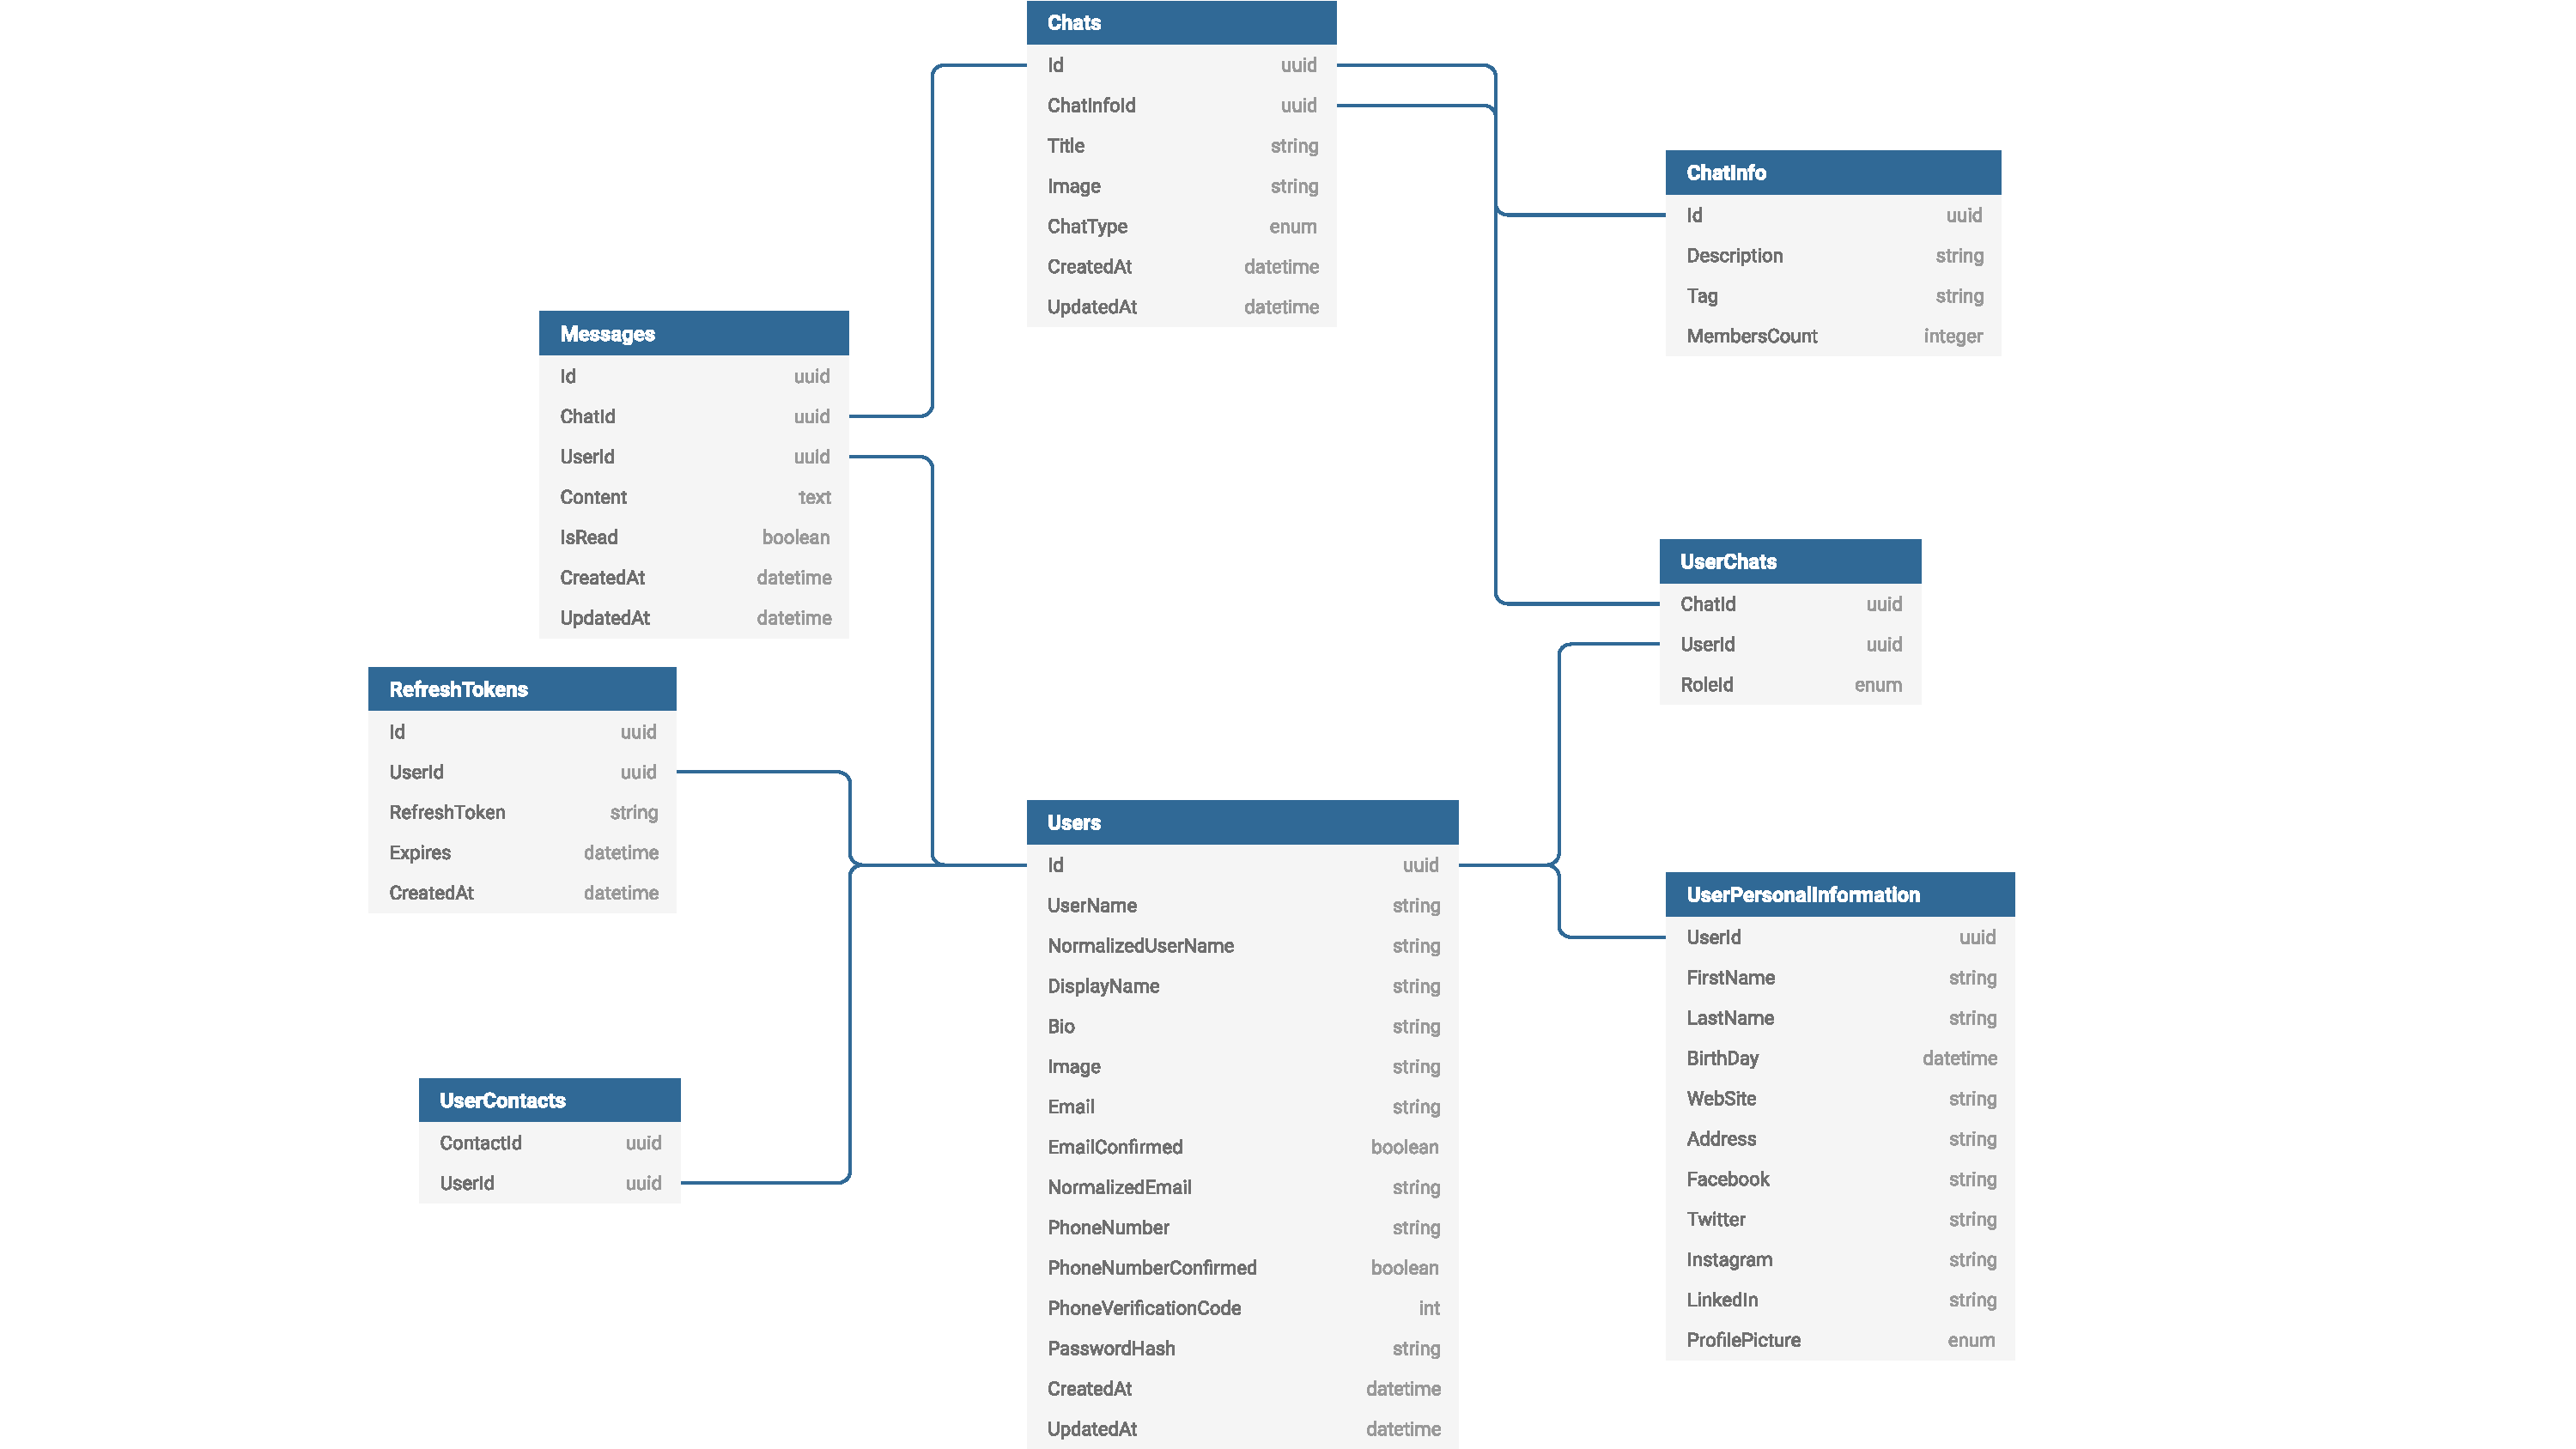
\includegraphics[width=1.2\textwidth]{Pictures/DB_diagram}
    \caption{Database diagram}\label{fig:figure5}
\end{figure}
Over whole data entities, we prefer to use universally unique identifier (UUID) or namely globally unique identifier (GUID),
a 128-bit label used for information in computer systems [\cite{leach2005universally}].
Simply, because it does not force us to keep a sequence on database side.
Sequence -- is a special entity provided in PostgreSQL relational databases.
It is responsible for generating unique values and sometimes causes a problems during migration of the database.
But still, are GUID identifiers are really always unique?
Well, each generated GUID is not guaranteed to be unique, the total number of unique keys $2^{128}$ or $3.4 \times 10^{38}$
is so large that the probability of the same number being generated twice is very small.
For example, consider the observable universe, which contains about $5 \times 10^{22}$ stars.
Every star could then have $6.8 \times 10^{15}$ universally unique GUIDs.
If you are scared of the same GUID values then put two of them next to each other.
If you are too paranoid then put three [\cite{GUIDSo}].


\section{Database Structure and related comments}\label{sec:database-structure-and-related-comments}
As a next topic to uncover goes the one related to the database structure.
Proper database structure is to be of very high priority, since it influences on the project as a whole,
starting from performance point of view and many other aspects.
When we say performance, we mean such a design of database that there is an opportunity to include required indexes,
depending on regularity of any particular request.
So, as the main topic of current thesis is implementation of Instant messaging system, we can list the following
general entities to be added to database schema.

\begin{itemize}
    \item \textbf{Users.} Table stores information about user.
    Table contains following columns:
    \begin{itemize}
        \item Id VARCHAR(36) -- Id of the user, primary key, GUID\@.
        \item UserName VARCHAR(50) -- Unique Username.
        \item NormalizedUserName VARCHAR(50) -- Unique Username in upper case.
        \item DisplayName VARCHAR(50) -- Name of the user, displayed to others.
        \item Bio VARCHAR(250) -- User's short biography, visible to others.
        \item Image VARCHAR(36) -- User's profile picture, visible to others.
        \item Email VARCHAR(120) -- User's email address, not public.
        \item EmailConfirmed BOOLEAN -- Flag that indicates if user has confirmed his email address.
        \item PhoneNumber VARCHAR(50) -- User's phone number.
        \item PhoneNumberConfirmed BOOLEAN -- Flag that indicates if user has confirmed his phone number.
        \item PhoneVerificationCode INTEGER -- Code sent to user in order to confirm phone number.
        \item PasswordHash VARCHAR(60) -- Hashed password.
        \item CreatedAt DATETIME -- Indicates the date and time user has been registered.
        \item UpdatedAt DATETIME -- Indicates the date and time user has updated his record.
    \end{itemize}
    \item \textbf{User Personal Information.} Table stores additional but not required info about user.
    Relation one-to-one with Users, foreign key is UserId, GUID\@.
    Table contains following columns:
    \begin{itemize}
        \item UserId VARCHAR(36) -- Foreign key to the Users table, GUID\@.
        \item FirstName VARCHAR(120) -- First name of user.
        \item LastName VARCHAR(120) -- Last name of user.
        \item BirthDay DATETIME -- Birth day of user.
        \item WebSite VARCHAR(120) -- Web site of user.
        \item Address VARCHAR(120) -- Residence address of user.
        \item Facebook VARCHAR(120) -- Facebook nickname of user.
        \item Twitter VARCHAR(120) -- Twitter nickname of user.
        \item Instagram VARCHAR(120) -- Instagram nickname of user.
        \item LinkedIn VARCHAR(120) -- LinkedIn nickname of user.
        \item ProfilePicture VARCHAR(36) -- Avatar of user.
    \end{itemize}
    \item \textbf{UserContacts.} Table stores the contacts of current user.
    Relation between tables Users and UserContacts is one-to-many, foreign key UserId.
    Table contains following columns:
    \begin{itemize}
        \item ContactId VARCHAR(36) -- Id of current user's contact, GUID\@.
        \item UserId VARCHAR(36) -- Id of current user, GUID\@.
    \end{itemize}
    \item \textbf{Chats.} In order to communicate with other people it is essentially to have a chat room.
    Our implementation provides chat rooms of the four types.
    Direct chat -- chat room between only two members.
    Public channel -- chat room for multiple members, each member can send and read messages.\ It displayed in search results.
    Readonly channel -- channel for multiple members, however only the owner can send messages.\ It displayed in search results.
    Private channel -- channel for multiple members, can be joined only by invite link.
    Each user can have a numerous various chats, however, each chat has a multiple members, at least 2 as the case of direct chat.
    Therefore, we consider a many-to-many relation between user and chats via intermediate table UserChats.
    We discuss UserChats relation in foregoing part.
    Continuing with Chats table, it contains the following columns:
    \begin{itemize}
        \item Id VARCHAR(36) -- Id of the chat, primary key, GUID.
        \item ChatInfoId VARCHAR(36) -- Since we have a four types of channels, which has a common subset of data,
        the different data is moved to another table, so it could be joined depending on chat type.
        For instance, any chat type except direct one would require to join additional data in order to display the chat properly.
        \item Title VARCHAR(50) -- Simply, the title of the chat.
        \item Image VARCHAR(36) -- Picture of the chat.\ Displayed in search results etc.
        \item ChatType ENUM -- The type of the chat, e.g direct chat, public channel, readonly channel, private channel.
        \item CreatedAt DATETIME -- Indicates the date and time chat has been created.
        \item UpdatedAt DATETIME -- Indicates the date and time chat has been updated.
    \end{itemize}
    \item \textbf{UserChats.} Table that considered as composite key of the many-to-many relation between Users and Chats tables.
    Over that, contains an enum value that indicates user's role in the chat.
    We assume the following user roles in the system:
    \begin{itemize}
        \item Owner -- the creator of the chat.
        Has an ultimate privileges.
        \item Administrator -- designated by the owner user, which has adjustable privileges.
        \item Moderator -- designated by administrator user, which has adjustable privileges.
        \item User -- default role assigned to the user on join the chat.
    \end{itemize}
    Despite that, the UserChats table contains the following columns:
    \begin{itemize}
        \item ChatId VARCHAR(36) -- Foreign key to the Chats table, GUID\@.
        \item UserId VARCHAR(36) -- Foreign key to the Users table, GUID\@.
        \item RoleId ENUM -- Indicates the user role in the chat, e.g Owner, Administrator, Moderator, User.
    \end{itemize}
    \item \textbf{Chat Info.} Table contains additional data related to the chat.
    This table is created since that we have four types of chats, namely, direct chat, public channel,
    readonly channel, private channel.
    These four types has a common data between each other.
    Common data between chat types is Chats table itself.
    One would advise to store the chats in a single table per chat type, however it is very costly approach, since there
    would be at least four joins per request.
    Note that every chat type except direct chat requires an additional data to be displayed, that is Chat Info.
    Contains following columns:
    \begin{itemize}
        \item Id VARCHAR(36) -- Id of the chat information, primary key, GUID\@.
        \item Description VARCHAR(120) -- Description of the chat.
        \item Tag VARCHAR(20) -- Unique identifier of the chat.
        \item MembersCount INTEGER -- Count of members in the chat.
    \end{itemize}
    \item \textbf{Messages.} Table that keeps messages and related data.
    Each chat has a multiple messages, however one message must belong only to single and defined chat,
    therefore relation between Chats and Messages is one-to-many, foreign key ChatId.
    From other side, each User has a multiple messages, however single message should belong to single author,
    therefore, we consider one-to-mane relation between Users and Messages, foreign key UserId.
    Messages table contains following columns:
    \begin{itemize}
        \item Id VARCHAR(36) -- Id of the message, primary key, GUID\@.
        \item ChatId VARCHAR(36) -- Foreign key to the Chats table, GUID\@.
        \item UserId VARCHAR(36) -- Foreign key to the Users table, GUID\@.
        \item Content VARCHAR(300) -- Content of the message.
        \item IsRead BOOLEAN -- Indicates whenever message has been read by another user.
        \item CreateAt DATETIME -- Time when the message has been created.
        \item UpdatedAt DATETIME -- Time when the message has been updated.
    \end{itemize}
    \item \textbf{Refresh Tokens.} Table stores refresh tokens.
    \begin{itemize}
        \item Id VARCHAR(36) -- Id of the token, primary key, GUID\@.
        \item UserId VARCHAR(39) -- Foreign key to the Users table, GUID\@.
        \item RefreshToken VARCHAR(60) -- Refresh token itself.
        \item Expires DATETIME -- Expiration date of refresh token.
        \item CreatedAt DATETIME -- Date when token has been created.
    \end{itemize}
\end{itemize}
Following diagram demonstrates the database structure.
\begin{figure}[H]
    \centering
    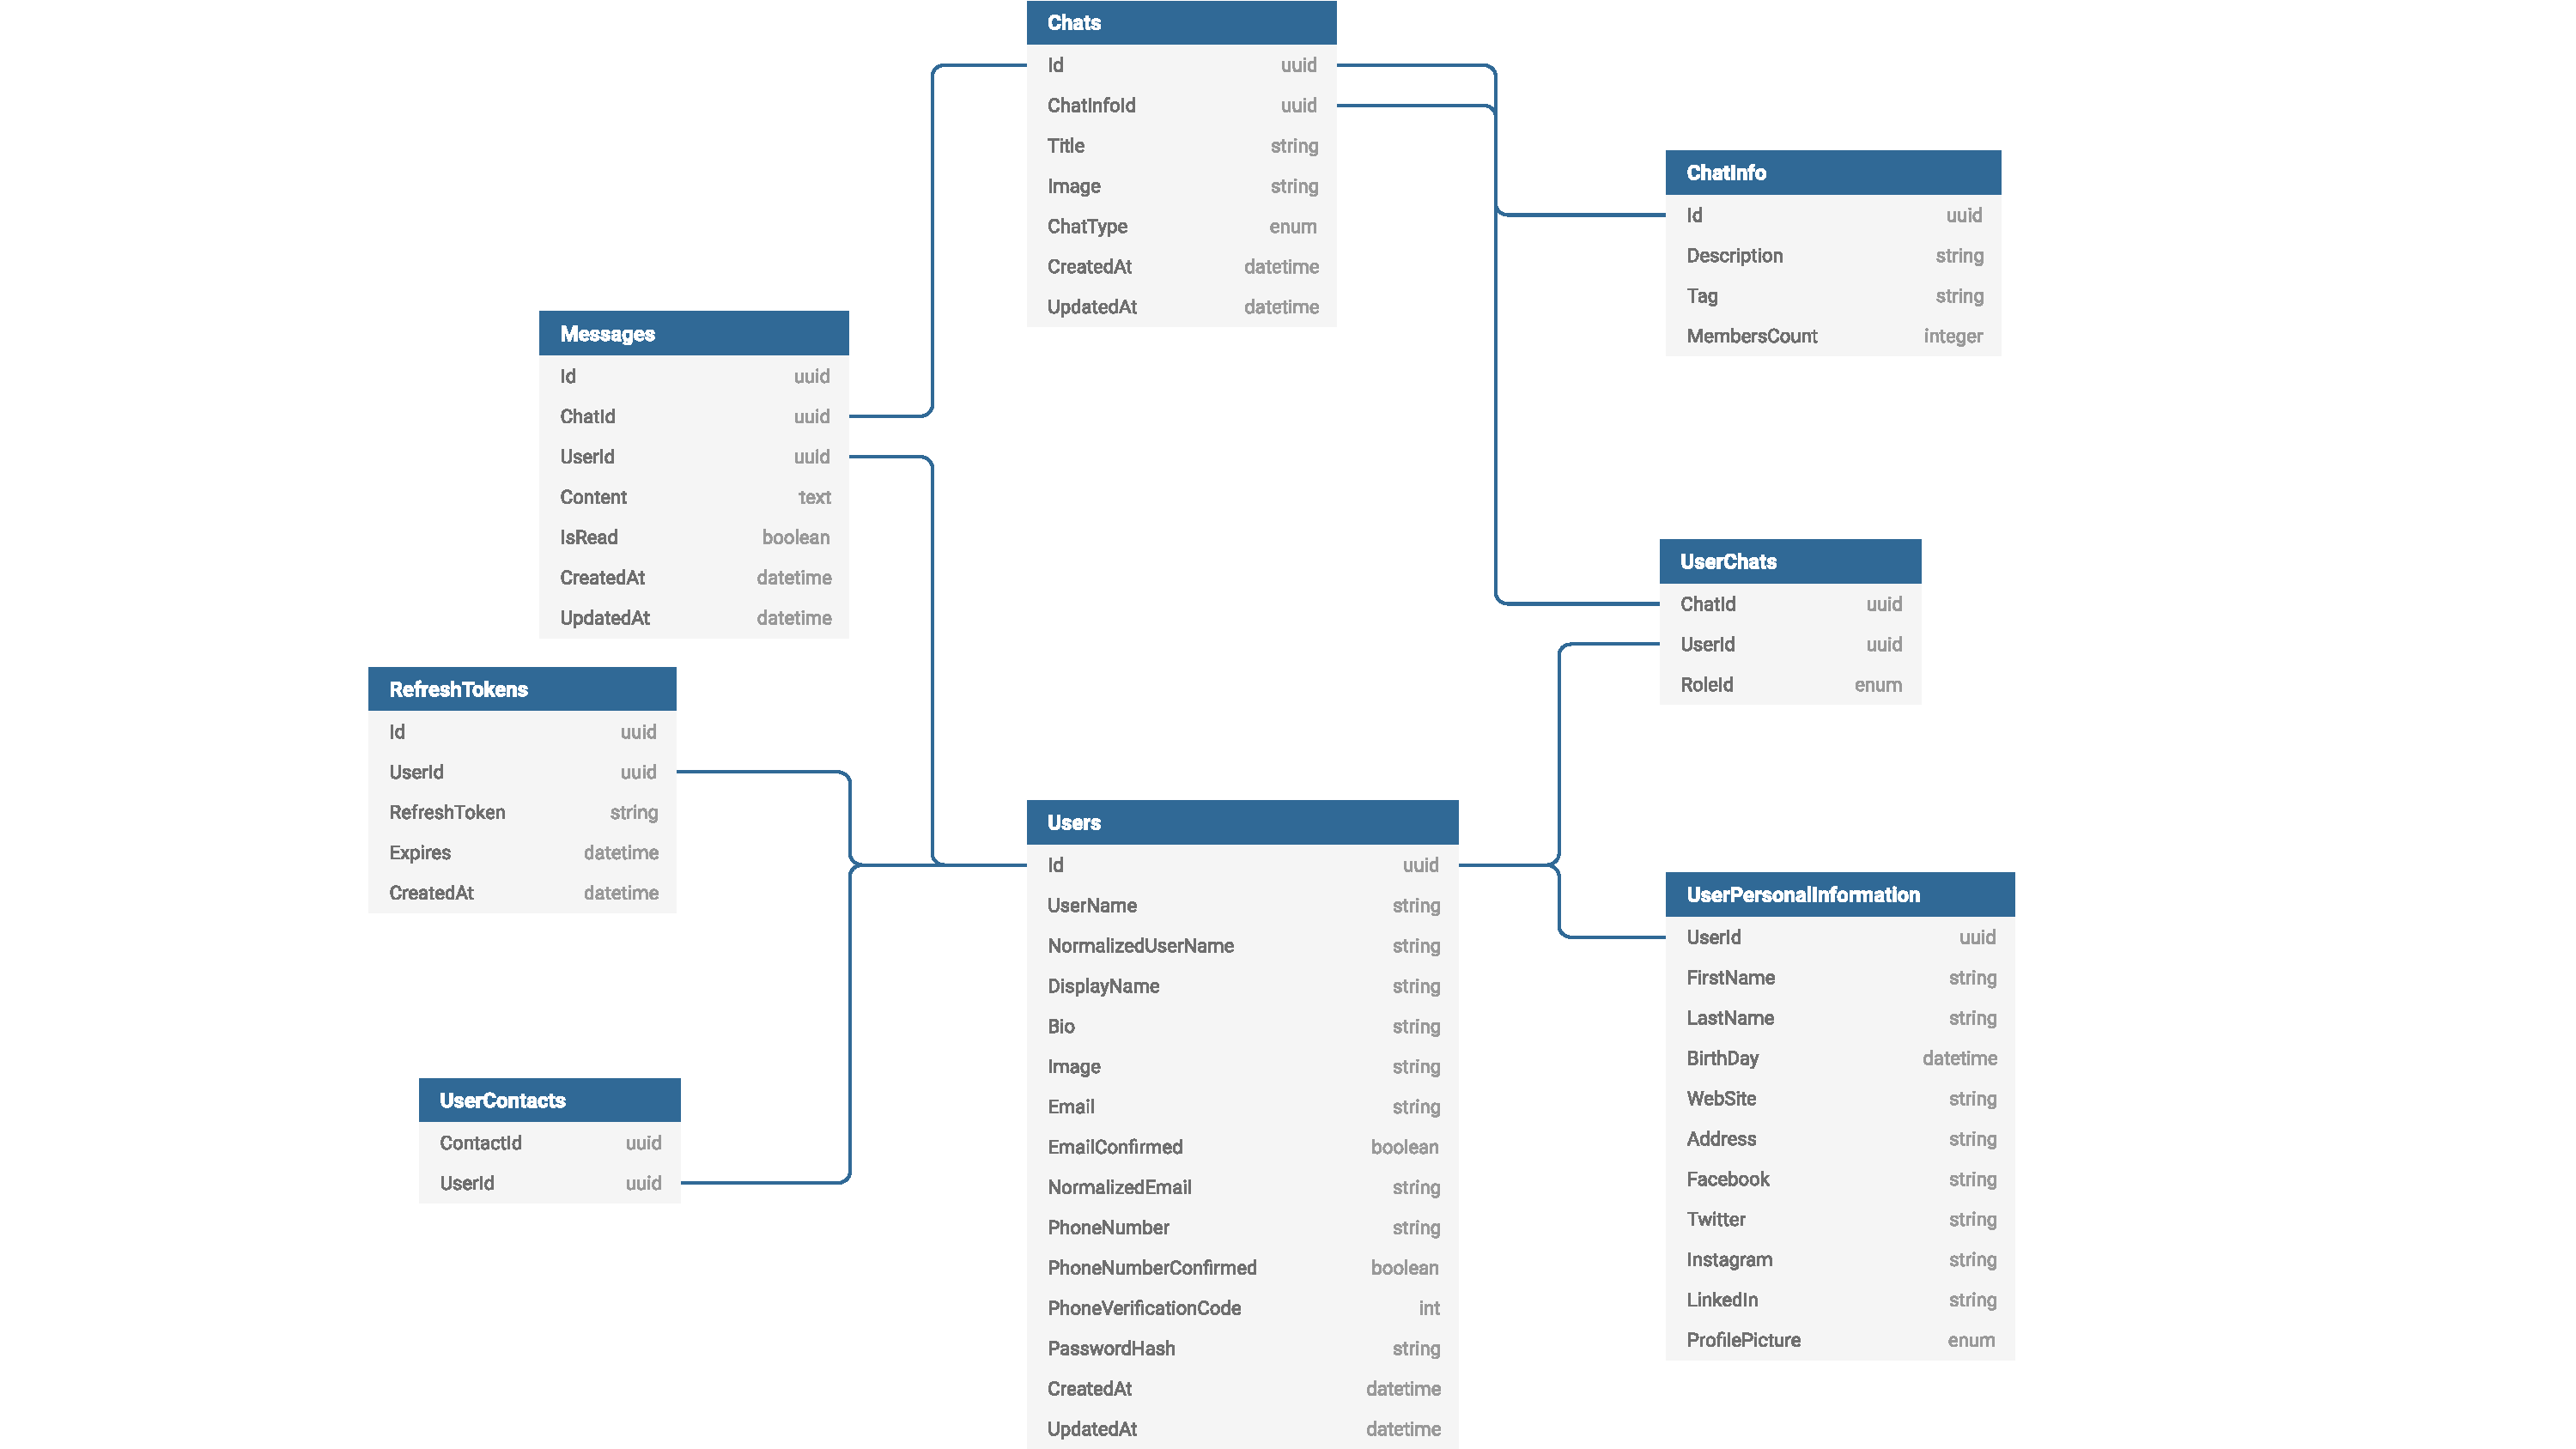
\includegraphics[width=1.2\textwidth]{Pictures/DB_diagram}
    \caption{Database diagram.}\label{fig:figure5}
\end{figure}


\section{Planned technologies}\label{sec:planned-technologies}
\begin{itemize}
    \item \textbf{SDK}: \href{https://dotnet.microsoft.com/download/dotnet/5.0}{.NET Core 5.0}
    \item \textbf{Database}
    \begin{itemize}
        \item SQL Database: \href{https://www.postgresql.org/}{PostgreSQL 13}
        \item ORM: \href{https://www.nuget.org/packages/Microsoft.EntityFrameworkCore/5.0.7?_src=template}{Entity Framework Core 5.0.7}
        \item PostgreSQL Provider: \href{https://www.nuget.org/packages/Npgsql.EntityFrameworkCore.PostgreSQL/5.0.7?_src=template}{Npgsql.EntityFrameworkCore.PostgreSQL 5.0.7}
    \end{itemize}
    \item \textbf{Authorization}
    \begin{itemize}
        \item JWT Library: \href{https://www.nuget.org/packages/System.IdentityModel.Tokens.Jwt}{System JWT 6.8.0}
        \item JWT Library: \href{https://www.nuget.org/packages/System.IdentityModel.Tokens}{System Tokens 6.11.1}
        \item JWT Bearer: \href{https://www.nuget.org/packages/Microsoft.AspNetCore.Authentication.JwtBearer/5.0.7?_src=template}{Microsoft Jwt Bearer 5.0.7}
    \end{itemize}
    \item \textbf{Infrastructure}
    \begin{itemize}
        \item Mediator Pattern Library: \href{https://www.nuget.org/packages/MediatR/9.0.0?_src=template}{MediatR 9.0.0}
        \item Validation Library: \href{https://www.nuget.org/packages/FluentValidation/10.2.3?_src=template}{Fluent Validation 10.2.3}
    \end{itemize}
    \item \textbf{Presentation}
    \begin{itemize}
        \item Documentation: \href{https://www.nuget.org/packages/Swashbuckle.AspNetCore/5.6.3?_src=template}{Swashbuckle 6.1.4}
        \item Realtime Communication: \href{https://www.nuget.org/packages/Microsoft.AspNet.SignalR/}{SignalR 2.4.2}
        \item FrontEnd Development: \href{https://angular.io/guide/setup-local}{Angular 11.2.7}
    \end{itemize}
    \item \textbf{Unit and Integration Testing}
    \begin{itemize}
        \item Testing Framework: \href{https://www.nuget.org/packages/NUnit/}{NUnit 3.13.1}
        \item Testing Auxiliary: \href{https://www.nuget.org/packages/Moq/}{Moq 4.16.1}
        \item Testing Auxiliary: \href{https://www.nuget.org/packages/FluentAssertions}{FluentAssertions 6.0.0}
    \end{itemize}
    \item \textbf{Static Code Analysis}: \href{https://www.sonarqube.org/downloads/}{SonarQube 8.9.2 LTS Community Edition}
    \item \textbf{Containerization}: \href{https://docs.docker.com/desktop/windows/install/}{Docker 3.6.0}
    \item \textbf{Continuous Integration}: \href{https://docs.github.com/en/actions}{GitHub Actions}
\end{itemize}


%    \chapter{Authentication and authorization}\label{ch:authentication-and-authorization}


\section{Motivation}\label{sec:motivation}
In this section we describe the processes of Authentication and Authorization in the system.
It is worth to remember the meaning of Authentication and Authorization definitions.
Authentication -- is the process of ascertaining that somebody really is who they claim to be [\cite{burrows1989logic}].
Authorization refers to rules that determine who is allowed to do what [\cite{fagin1978authorization}].
For example, Adam may be authorized to create and delete databases, while Eve is only authorized to read.
The two concepts are completely orthogonal and independent, but both are central to security design, and the
failure to get either one correct opens up the avenue to compromise.
In terms of web apps, very crudely speaking, authentication is when you check login credentials to see if you recognize
a user as logged in, and authorization is when you look up in your access control whether you allow the user to view,
edit, delete or create content.
Currently, there are two widely-known authentication methods, that are cookie authentication and JWT (JSON Web Token)
authentication.
We discuss JWTs in next section.


\section{JWT Tokens}\label{sec:jwt-tokens}
JSON Web Token (JWT) is an open standard (RFC 7519) that defines a compact and self-contained way for securely
transmitting information between parties as a JSON object [\cite{jones2015json}].
This information can be verified and trusted because it is digitally signed.
JWTs can be signed using a secret (with the HMAC algorithm [\cite{wang2004hmac}]) or a public/private key pair using RSA or ECDSA\@.
Although JWTs can be encrypted to also provide secrecy between parties, we will focus on signed tokens.
Signed tokens can verify the integrity of the claims contained within it, while encrypted tokens hide those claims from
other parties.
When tokens are signed using public/private key pairs, the signature also certifies that only the party holding the
private key is the one that signed it.
In its compact form, JSON Web Tokens consist of three parts separated by dots, which are:
\begin{itemize}
    \item Header -- typically consists of two parts: the type of the token, which is JWT, and the signing algorithm
    being used, such as HMAC SHA256 or RSA\@.
    \item Payload -- The second part of the token is the payload, which contains the claims.
    Claims are statements about an entity (typically, the user) and additional data.
    There are three types of claims: registered, public, and private claims.
    \item Signature -- To create the signature part you have to take the encoded header, the encoded payload, a secret,
    the algorithm specified in the header, and sign that.
\end{itemize}
Therefore, a JWT typically looks like \texttt{xxxxx.yyyyy.zzzzz}.
Then, this JSON is Base64Url encoded to form the first part of the JWT\@.

As to the projects concerns, we should handle multiple client applications, e.g desktop,
web, mobile etc.
Therefore, cookie authorization doesn't fit for the project, however the JWT one surely passes.


\section{JWT Authentication}\label{sec:jwt-authentication}
Authentication (from the Greek [authentikos] - real, genuine;
by [authentes] - author) - it is process which verify user credentials, for instance login and password.
User authentication by comparing the login and password entered by him with the data saved in the database.
Authorization - it is process which check of the user's rights to access certain resources.

For example, after authentication the user Bob gets the right to access and get from resource
https://resource.com some data.
When the user Bob accesses to the vip resource, the authorization system will check has the user right to access
this resource.

\begin{enumerate}
    \item The user with email bob@gmail.com successfully authenticated.
    \item The server checks in database roles of Bob.
    \item The server generated token with specified role.
    \item Bob go in a certain resource using received token.
    \item The server check user rights in token and respectively skips or cuts the request.
\end{enumerate}

The fifth point is the authorization.
JSON Web Token (JWT) contains 3 blocks separated by dots: header, payload and signature.
The first 2 blocks presented in JSON-format and additionally encoded to the format base64.
Payload contains arbitrary key-value pairs.
The JWT standard defines several reserved names: iss, aud, exp, and others.
Signature can be generated with help of symmetric and asymmetric encryption algorithms.
In addition, there is a separate standard that describes the format of the encrypted JWT-token.
Tokens present a means of authorization for every request from client to server.
Tokens are generated on the server based on secret key which stored in the server and payload.
As a result, token stored on the client and used when it is necessary to authorize any requests.

When a hacker tries to replace the data in the header or payload, token will become invalid, since the signature
will not match the original values and the hacker does not ability to generate a new signature,
since the encryption secret key stored in the server.

Access Token is used for request authorization and for storing the additional information about user, for example,
User ID, Display Name and others.
This information is also called payload.
All payload fields is free set of fields necessary for implementation your private business logic.
That is User ID, Display Name is not required fields and presents only a special case.

Refresh Token issued by server based on successful authentication results and used for get new access/refresh token pair.
Every token has its own lifetime.
For example, Access token lifetime may be 5 minutes, and Refresh token's 7 days.
Since tokens are not encrypted information, it is highly not recommended to store any sensitive data in them, for example,
password hashes, payment credentials, etc.

\subsection{Creating sessions}\label{subsec:creating-sessions}

\begin{enumerate}
    \item The user logs into the application by transferring the login, password and fingerprint of the browser,
    or some other unique device identifier if it is not a browser.
    \item The server verifies the authenticity of the login and password.
    \item If successful, creates and writes a session to the database, see table session in [reference database schema].
    \item The server generates Access token.
    \item The server sends to client access token and refresh token, UUID\@.
    \item Client saves the pair of access and refresh tokens.
\end{enumerate}

Before each request client preliminarily checks access token's lifetime and if it expired, client sends request for
updating access token.
For more confidence, we can update tokens a few seconds earlier.
That is, the case when the API receives an expired access token is practically excluded.
To use the authentication feature on more than one device, it is necessary to store all refresh tokens for each user.
The following diagram demonstrates discussed processes

\begin{figure}[H]
    \centering
    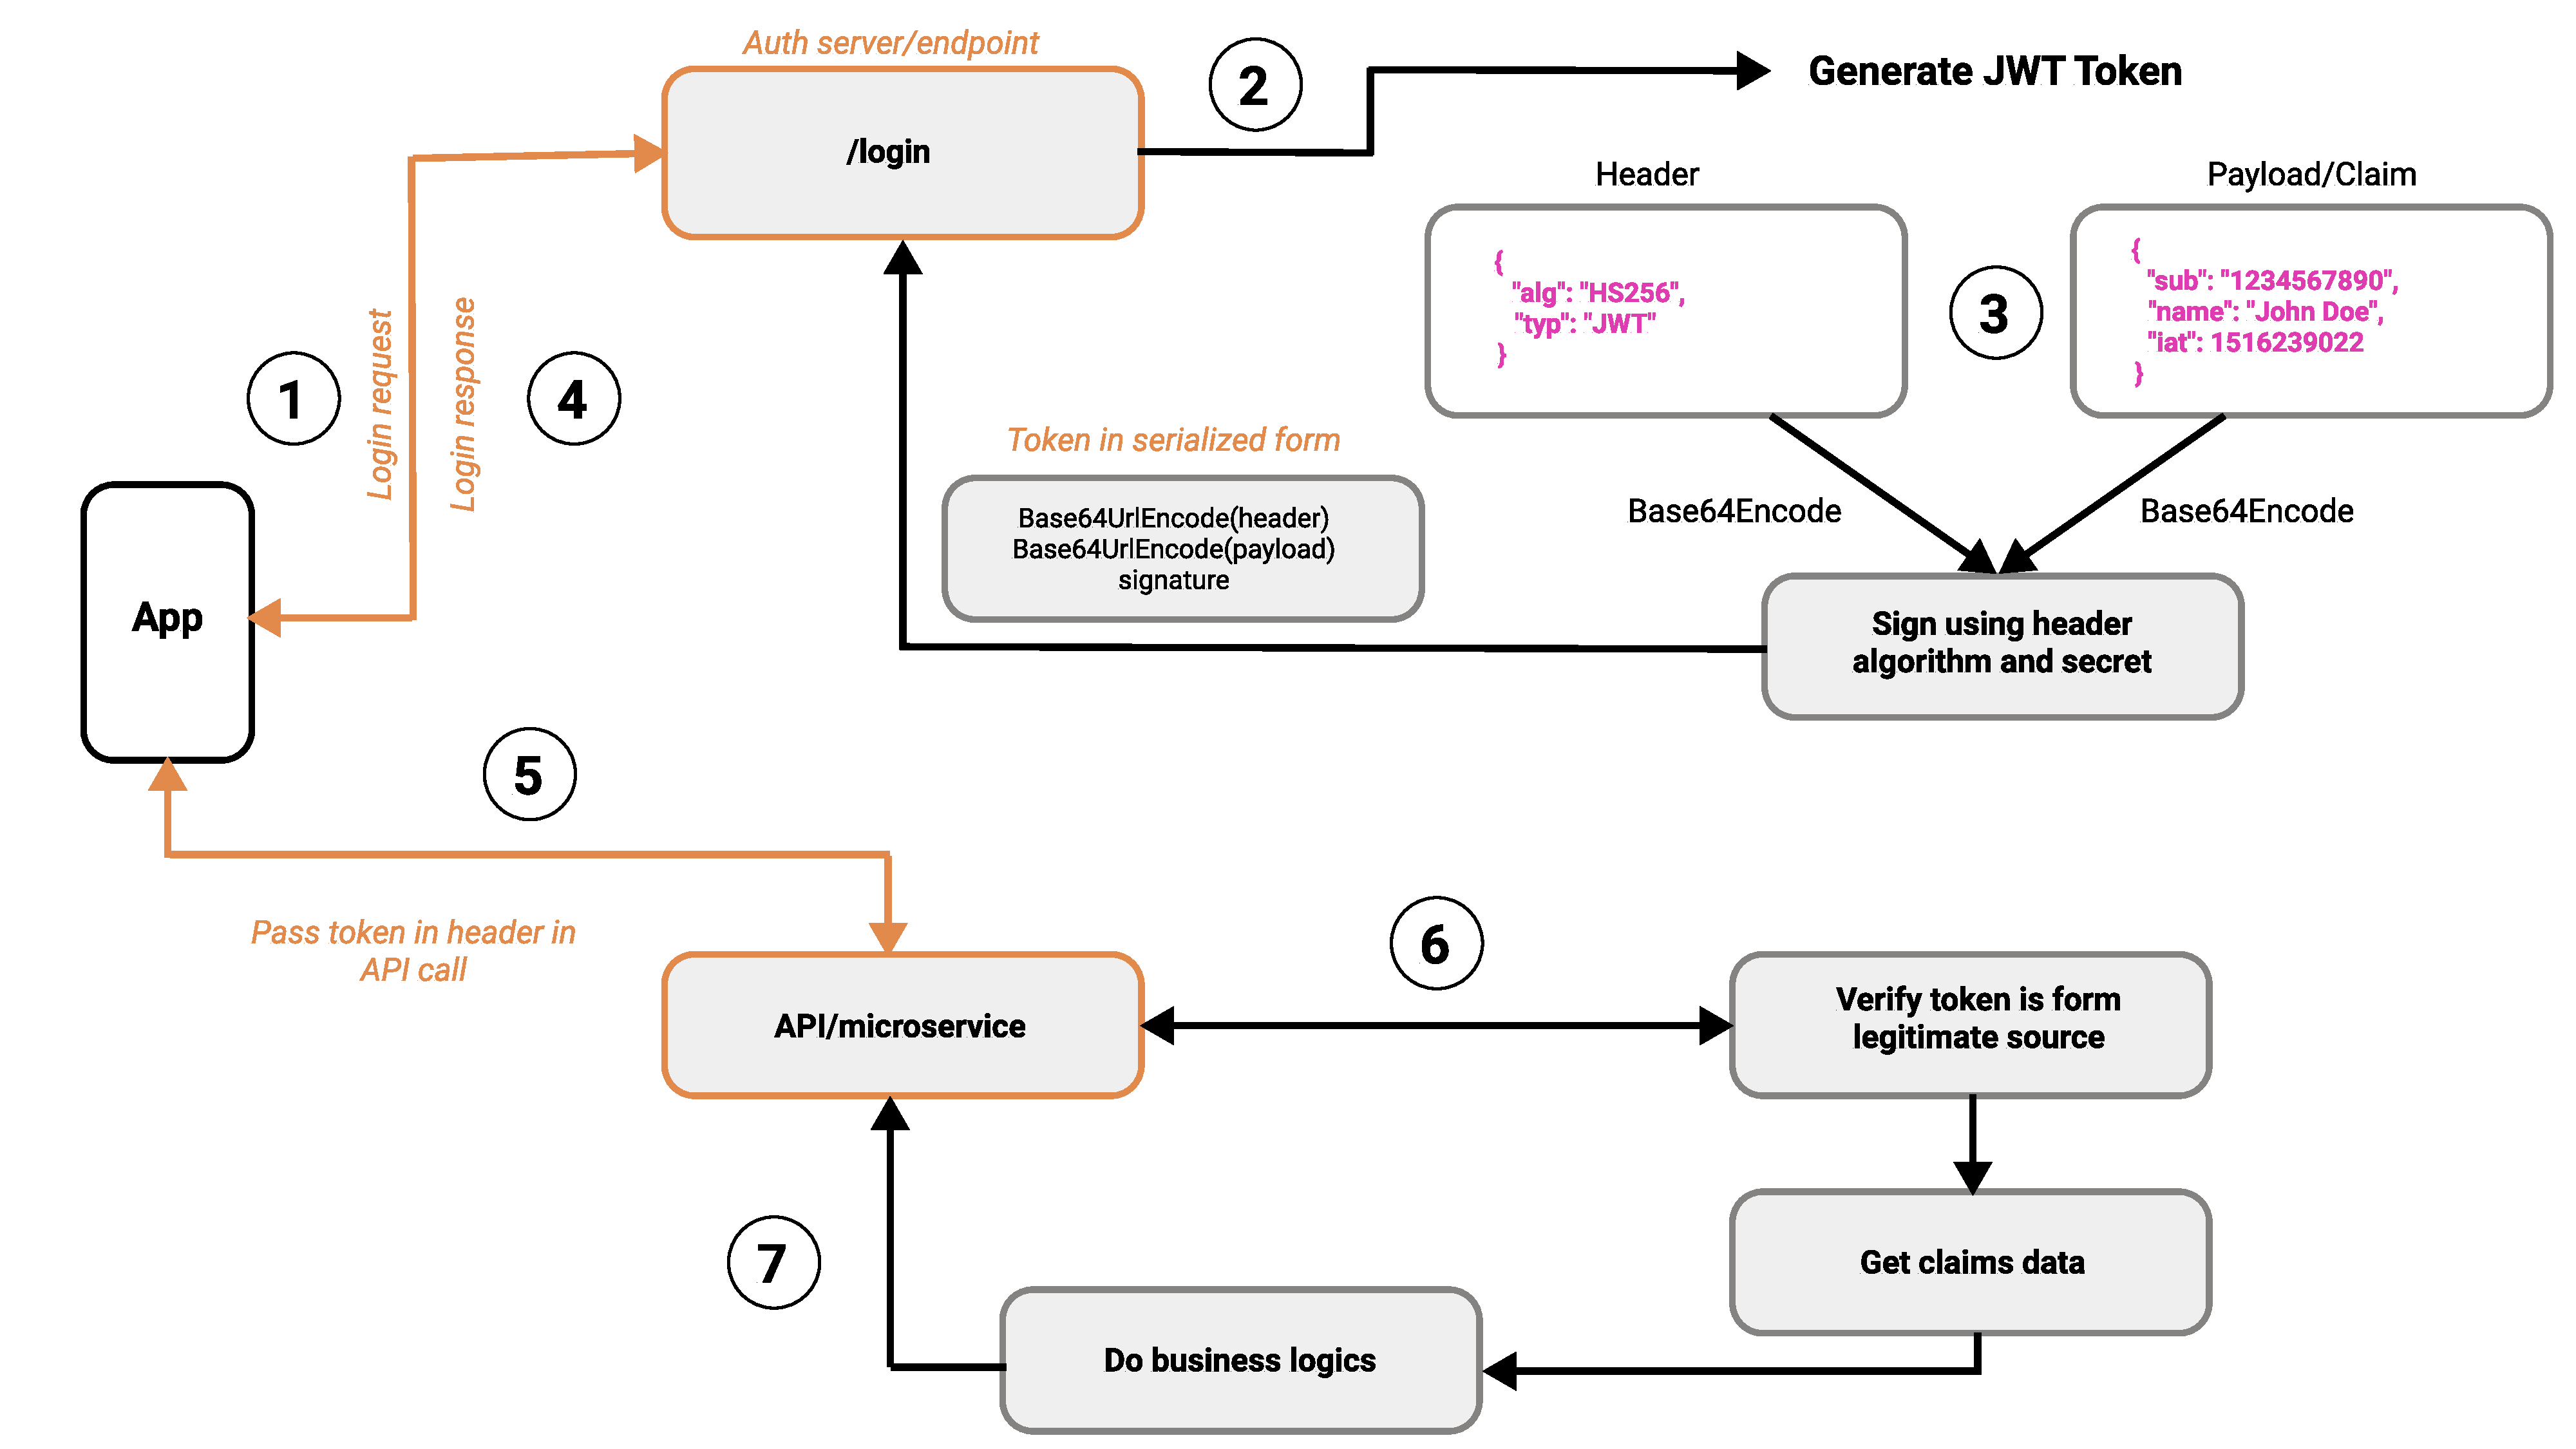
\includegraphics[width=1\textwidth]{Pictures/jwt_auth_scheme.pdf}
    \caption{JWT Authentication principle diagram.}\label{fig:figure3}
\end{figure}

Also, it is worth to add a few basic rules about JWT usage [\cite{RDegges}]
\begin{itemize}
    \item JWT should have a short lifetime, since it cannot be revoked.
    \item JWT should be used in a single time, e.g JWT per request.
\end{itemize}
%    \chapter{Security aspects of communication channel}\label{ch:security-aspects-of-communication-channel}


\section{Discussion on HTTPS Protocol}\label{sec:discussion-on-https-protocol}
HTTPS stands for Hypertext Transfer Protocol Secure.
HTTPS is an extension of the Hypertext Transfer Protocol.
It is used for secure communication over a computer network,
and is widely used on the Internet [\cite{lam2000secure, karayiannis2019implementing}].
In HTTPS, the communication protocol is encrypted using Transport Layer Security [\cite{turner2014transport}]
or, formerly, Secure Sockets Layer [\cite{weaver2006secure}].
The protocol is therefore also referred to as HTTP over TLS or HTTP over SSL\@.
The principal motivations for HTTPS are authentication of the accessed website, and protection of the privacy and integrity
of the exchanged data while in transit.
It protects against \textit{man-in-the-middle attacks}.
The bidirectional encryption of communications between a client and server protects the communications against
eavesdropping and tampering [\cite{mayer2016tlscompare, jiang2019physical}].
The authentication aspect of HTTPS requires a trusted third party to sign server-side digital certificates.
This was historically an expensive operation, which meant fully authenticated HTTPS connections were usually found only
on secured payment transaction services and other secured corporate information systems on the World Wide Web.
In 2016, a campaign by the Electronic Frontier Foundation with the support of web browser developers led to the protocol
becoming more prevalent [\cite{he2014shadowcrypt}].
HTTPS is now used more often by web users than the original non-secure HTTP, primarily to protect
page authenticity on all types of websites;
secure accounts;
and to keep user communications, identity, and web browsing private [\cite{rescorla2000rfc2818}].

\subsection{What is an SSL Certificate?}\label{subsec:what-is-an-ssl-certificate?}
SSL stands for Secure Sockets Layer and, in short, it's the standard technology for keeping an internet connection
secure and safeguarding any sensitive data that is being sent between two systems, preventing criminals from reading
and modifying any information transferred, including potential personal details.
The two systems can be a server and a client, for example, a shopping website and browser, or server to server,
for example, an application with personal identifiable information or with payroll information.
SSL certificates are what enable websites to move from HTTP to HTTPS, which is more secure.
An SSL certificate is a data file hosted in a website's origin server.
SSL certificates make SSL or TLS (Transport Layer Security) encryption possible, and they contain the website's
public key and the website's identity, along with related information.
Devices attempting to communicate with the origin server will reference this file to obtain the public key and verify
the server's identity.
The private key is kept secret and secure.
SSL certificates include:
\begin{itemize}
    \item The domain name that the certificate was issued for
    \item Which person, organization, or device it was issued to
    \item Which certificate authority issued it
    \item The certificate authority's digital signature
    \item Associated sub-domains
    \item Issue date of the certificate
    \item Expiration date of the certificate
    \item The public key (the private key is kept secret)
\end{itemize}
The public and private keys used for SSL are essentially long strings of characters used for encrypting and decrypting data.
Data encrypted with the public key can only be decrypted with the private key, and vice versa.
\begin{figure}[H]
    \centering
    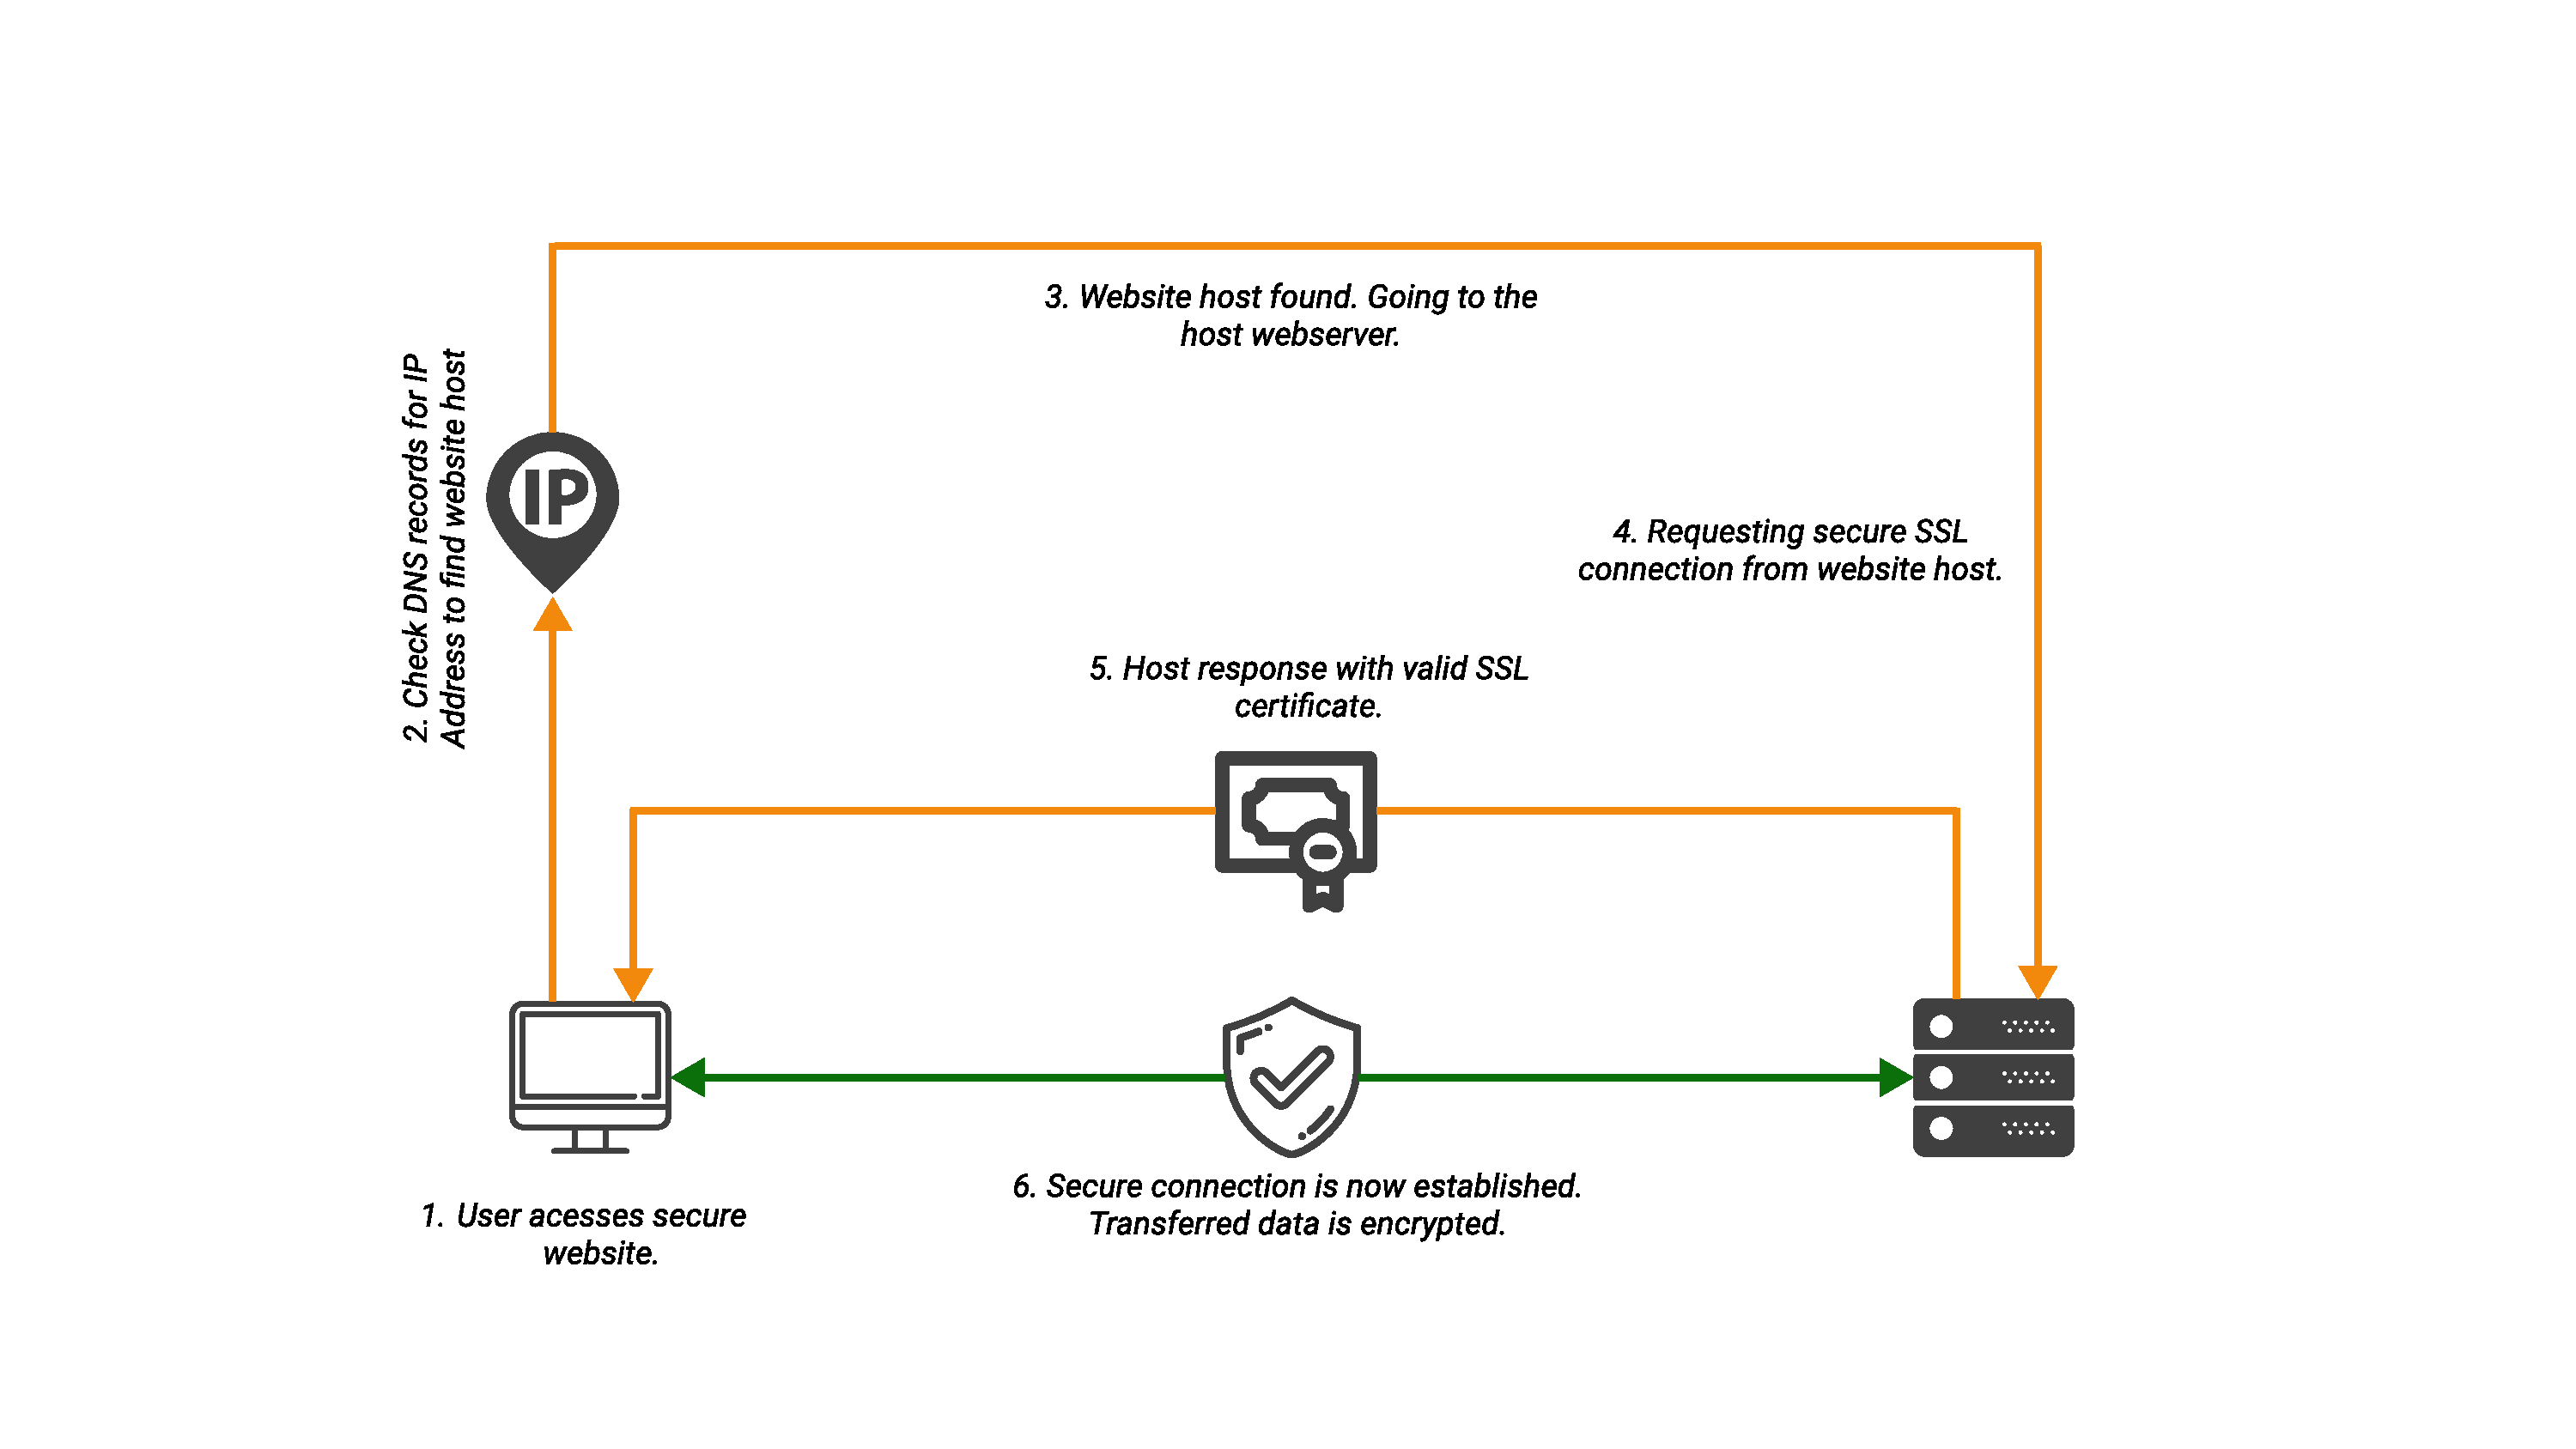
\includegraphics[width=1\textwidth]{Pictures/HTTPS_Flow}
    \caption{HTTPS flow diagram.}\label{fig:figure6}
\end{figure}

\subsection{Discussion on E2E Encryption}\label{subsec:discussion-on-e2e-encryption-over-https-protocol}
Discuss here about why it is useless to implement E2E encryption in web version,
however is ok to implement for mobile one [\cite{JsMathRandom, E2eVsTLS}].
Answer the questions:
\begin{itemize}
    \item \textbf{What is End-to-End (E2E) Encryption?}
    End-to-end encryption (E2EE) is a system of communication where only the communicating users can read the messages.
    In principle, it prevents potential eavesdroppers -- including telecom providers, Internet providers,
    and even the provider of the communication service -- from being able to access the cryptographic keys needed to
    decrypt the conversation.
    End-to-end encryption is intended to prevent data being read or secretly modified, other than by the true sender and
    recipient.
    The messages are encrypted by the sender but the third party does not have a means to decrypt them, and stores them
    encrypted.
    The recipients retrieve the encrypted data and decrypt it themselves.
    Because no third parties can decipher the data being communicated or stored, for example, companies that provide
    end-to-end encryption are unable to hand over texts of their customers' messages to the authorities.

    It is important to note that E2EE does not equal privacy or security.
    In many messaging systems, including email and many chat networks, messages pass through intermediaries and are stored
    by a third party, from which they are retrieved by the recipient.
    Even if the messages are encrypted, they are only encrypted 'in transit', and are thus accessible by the service provider,
    regardless of whether server-side disk encryption is used.
    Server-side disk encryption simply prevents unauthorized users from viewing this information.
    It does not prevent the company itself from viewing the information, as they have the key and can simply decrypt this data.
    This allows the third party to provide search and other features, or to scan for illegal and unacceptable content,
    but also means they can be read and misused by anyone who has access to the stored messages on the third party system,
    whether this is by design or via a backdoor.
    This can be seen as a concern in many cases where privacy is very important, such as businesses whose reputation
    depends on their ability to protect third party data, negotiations and communications that are important enough to
    have a risk of targeted 'hacking' or surveillance, and where sensitive subjects such as health, and information about
    minors are involved.
    \item \textbf{E2E Encryption in Telegram messenger.} Telegram uses so-called MTProto 2.0 cryptographic protocol.
    Before a message (or a multipart message) is transmitted over a network using a transport protocol, it is encrypted
    in a certain way, and an external header is added at the top of the message that consists of a 64-bit key identifier
    \textbf{auth\_key\_id} (that uniquely identifies an authorization key for the server as well as the user) and
    a 128-bit message key \textbf{msg\_key}.
    The authorization key \textbf{auth\_key} combined with the message key \textbf{msg\_key} define an actual 256-bit
    key \textbf{aes\_key} and
    a 256-bit initialization vector \textbf{aes\_iv}, which are used to encrypt the message using AES-256 encryption in
    infinite garble extension (IGE) mode.
    Note that the initial part of the message to be encrypted contains variable data
    (session, message ID, sequence number, server salt) that obviously influences the message key and thus the AES key
    and IV\@.
    In MTProto 2.0, the message key is defined as the 128 middle bits of the SHA-256 of the message body
    (including session, message ID, padding, etc.) prepended by 32 bytes taken from the authorization key.
    In the older MTProto 1.0, the message key was computed as the lower 128 bits of SHA-1 of the message body,
    excluding the padding bytes.
    Where
    \begin{itemize}
        \item \textbf{Authorization Key (auth\_key).} A 2048-bit key shared by the client device and the server,
        created upon user registration directly on the client device by exchanging Diffie-Hellman keys, and never
        transmitted over a network.
        Each authorization key is user-specific.
        There is nothing that prevents a user from having several keys that correspond to "permanent sessions"
        on different devices, and some of these may be locked forever in the event the device is lost.
        \item \textbf{Server Key.} A 2048-bit RSA key used by the server digitally to sign its own messages while
        registration is underway and the authorization key is being generated.
        The application has a built-in public server key which can be used to verify a signature but cannot be used
        to sign messages.
        A private server key is stored on the server and changed very infrequently.
        \item \textbf{Key Identifier (auth\_key\_id).} The 64 lower-order bits of the SHA1 hash of the authorization
        key are used to indicate which particular key was used to encrypt a message.
        Keys must be uniquely defined by the 64 lower-order bits of their SHA1, and in the event of a collision,
        an authorization key is regenerated.
        A zero key identifier means that encryption is not used which is permissible for a limited set of message types
        used during registration to generate an authorization key in a Diffie-Hellman exchange.
        For MTProto 2.0, SHA1 is still used here, because auth\_key\_id should identify the authorization key used
        independently of the protocol version.
        \item \textbf{Session.} A (random) 64-bit number generated by the client to distinguish between individual
        sessions (for example, between different instances of the application, created with the same authorization key).
        The session in conjunction with the key identifier corresponds to an application instance.
        The server can maintain session state.
        Under no circumstances can a message meant for one session be sent into a different session.
        The server may unilaterally forget any client sessions;
        clients should be able to handle this.
        \item \textbf{Server Salt.} A (random) 64-bit number changed every 30 minutes (separately for each session) at
        the request of the server.
        All subsequent messages must contain the new salt although, messages with the old salt are still accepted for
        a further 1800 seconds.
        Required to protect against replay attacks and certain tricks associated with adjusting the client clock to
        a moment in the distant future.
        \item \textbf{Message Identifier (msg\_id).} A (time-dependent) 64-bit number used uniquely to identify a
        message within a session.
        Client message identifiers are divisible by 4, server message identifiers modulo 4 yield 1 if the message is a
        response to a client message, and 3 otherwise.
        Client message identifiers must increase monotonically within a single session, the same as server message
        identifiers, and must approximately equal $unixtime \times 2^{32}$.
        This way, a message identifier points to the approximate moment in time the message was created.
        A message is rejected over 300 seconds after it is created or 30 seconds before it is created
        this is needed to protect from replay attacks.
        In this situation, it must be re-sent with a different identifier or placed in a container with a higher identifier.
        The identifier of a message container must be strictly greater than those of its nested messages.
    \end{itemize}
    \item Does it make sense to implement it for web version?
    \item Does it make sense to implement it for mobile version?
    \item Why is it not worth that to implement E2E for web version?
\end{itemize}


\section{Diffie-Hellman Key Exchange}\label{sec:diffie-hellman-key-exchange}
Diffie–Hellman key exchange [\cite{li2010research}] is a method of securely exchanging cryptographic keys over a public channel
and was one of the first public-key protocols
as conceived by Ralph Merkle and named after Whitefield Diffie and Martin Hellman.
DH is one of the earliest practical examples of public key exchange implemented within the field of cryptography.
Published in 1976 by Diffie and Hellman, this is the earliest publicly known work that proposed the idea of a private
key and a corresponding public key.
Traditionally, secure encrypted communication between two parties required that they first exchange keys by some secure physical means,
such as paper key lists transported by a trusted courier.
The Diffie–Hellman key exchange method allows two parties that have no prior knowledge of
each other to jointly establish a shared secret key over an insecure channel.
This key can then be used to encrypt subsequent communications using a symmetric-key cipher.
Although Diffie–Hellman key agreement itself is a non-authenticated key-agreement protocol, it provides the basis for a
variety of authenticated protocols, and is used to provide forward secrecy in Transport Layer Security's ephemeral modes,
referred to as EDH or DHE [\cite{ahirwal2013elliptic}] depending on the cipher suite.

Diffie–Hellman key exchange establishes a shared secret between two parties that can be used for secret communication
for exchanging data over a public network.
An analogy illustrates the concept of public key exchange by using colors instead of very large numbers:
\begin{figure}[H]
    \centering
    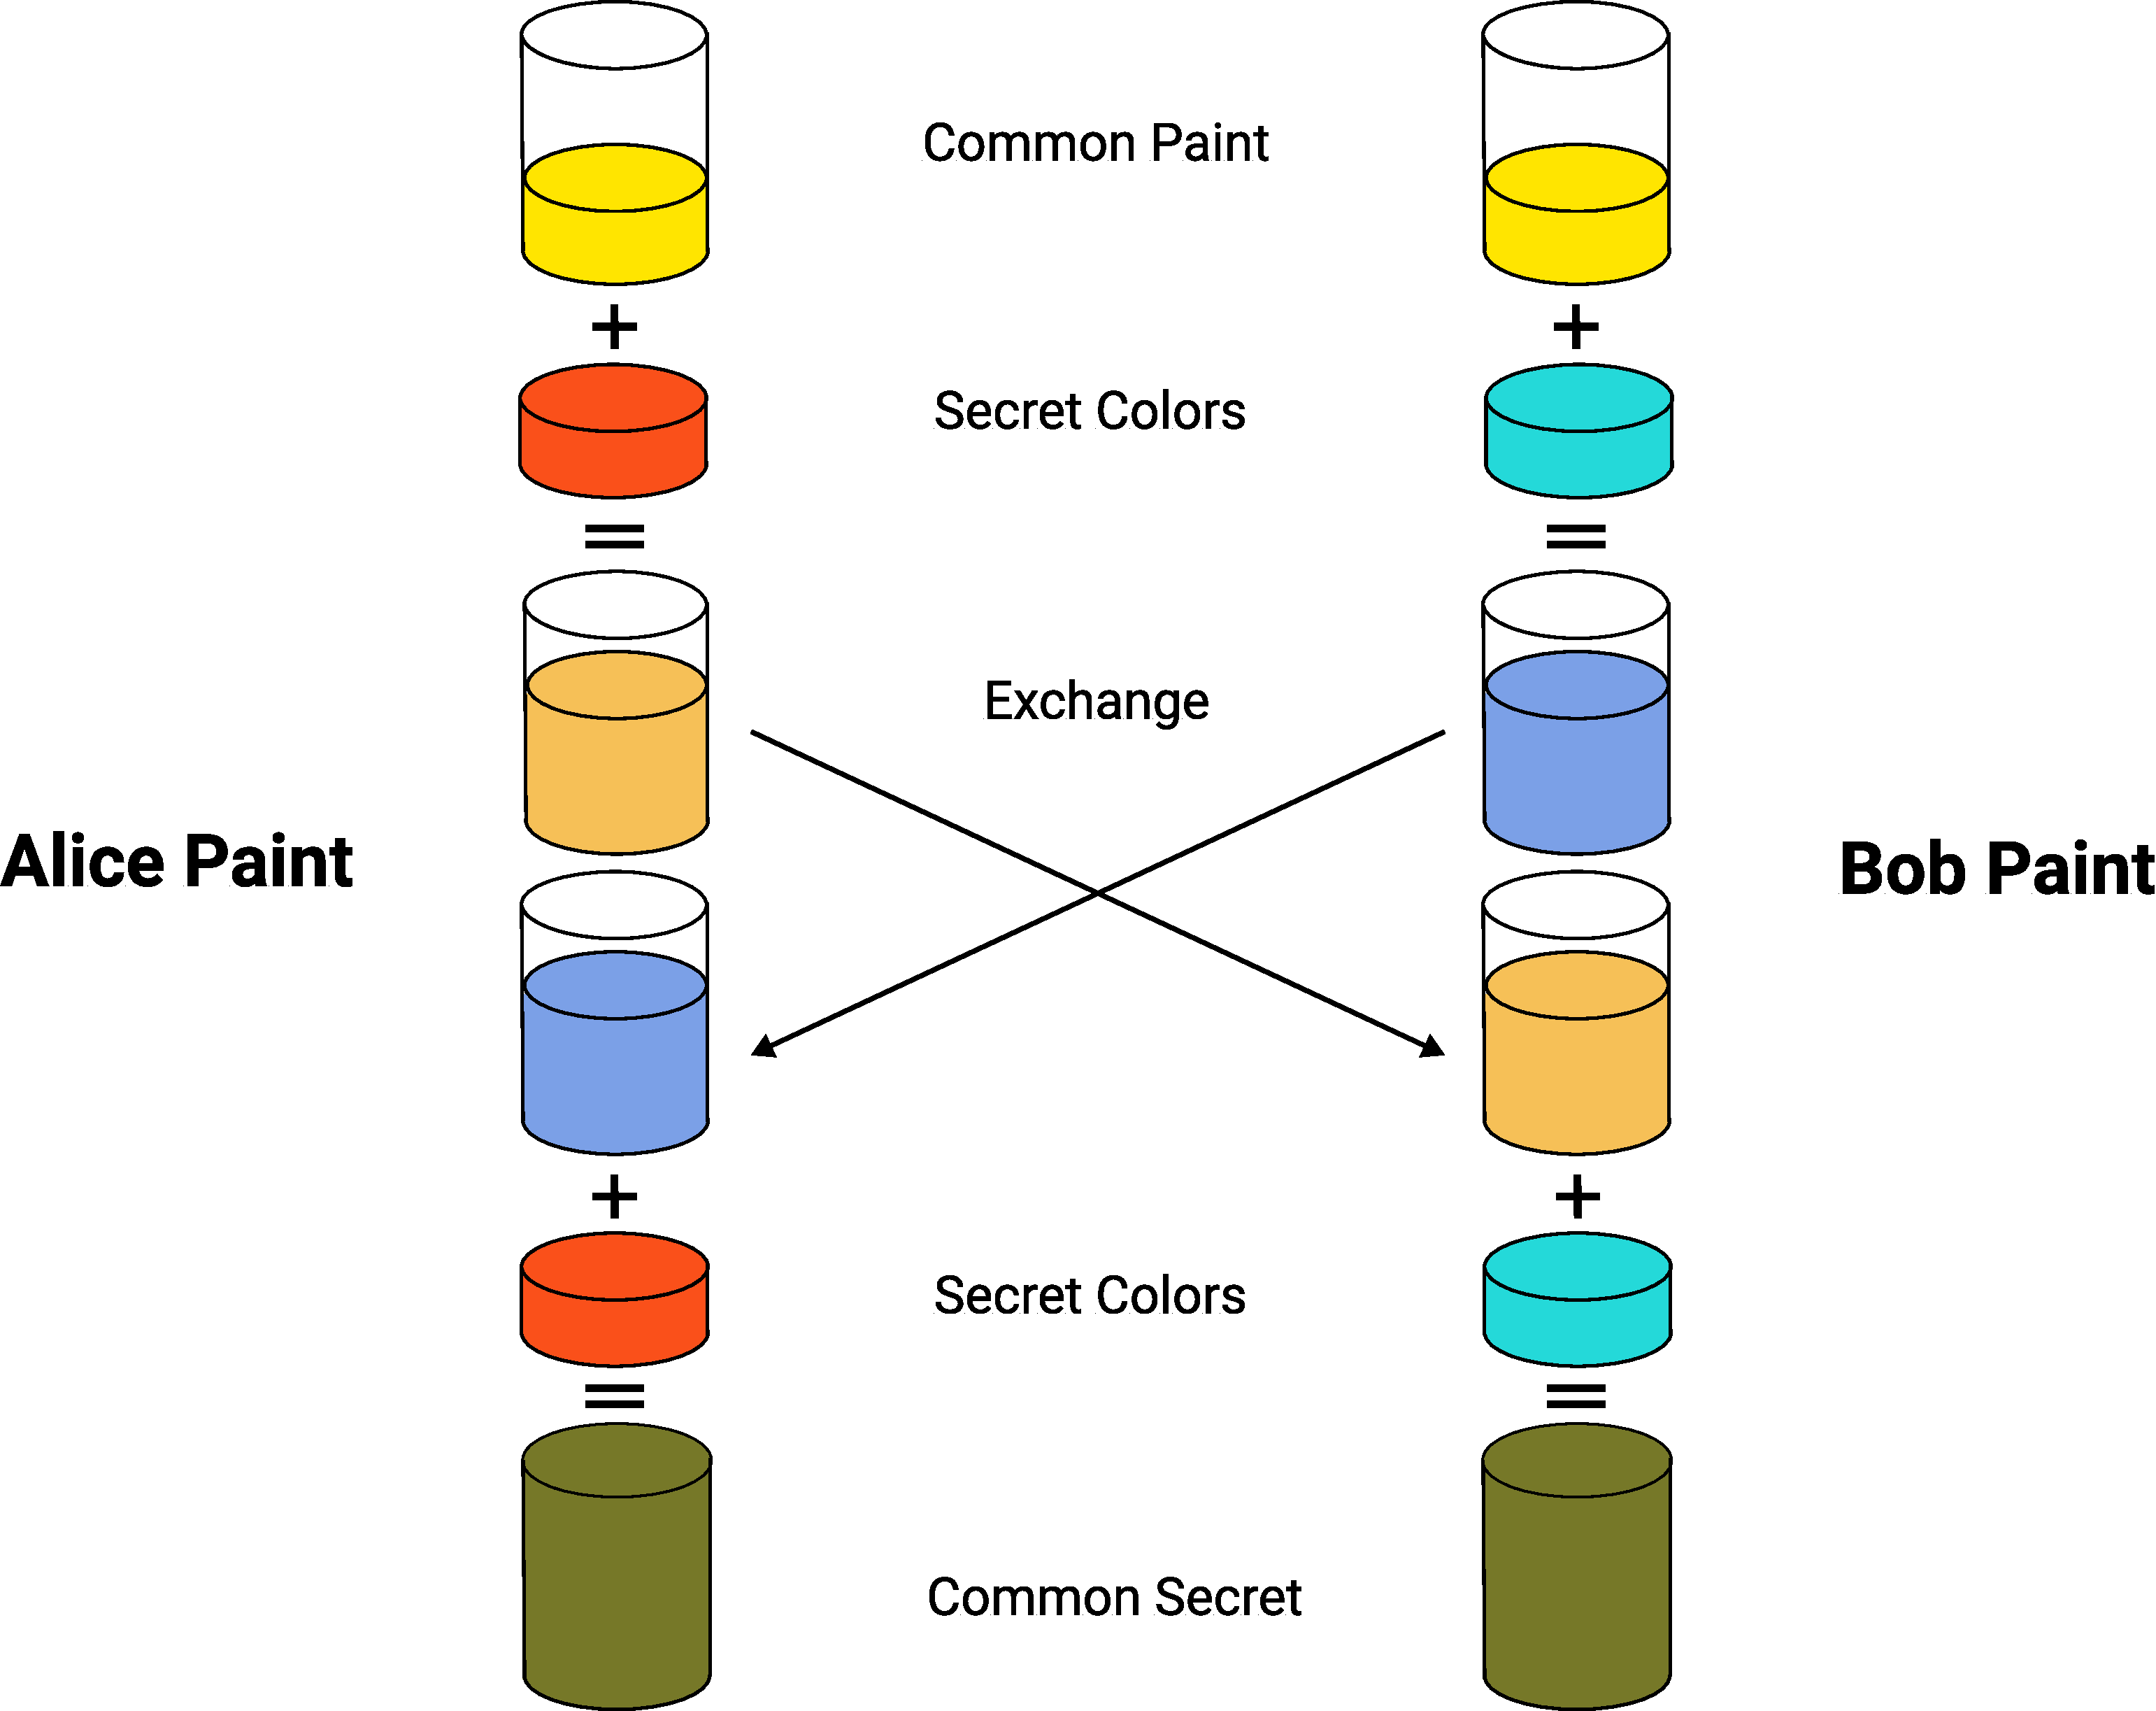
\includegraphics[width=1\textwidth]{Pictures/Diffie-Hellman}
    \caption{Illustration of the concept behind Diffie–Hellman key exchange. Source: }\label{fig:figure4}
\end{figure}
The process begins by having the two parties, Alice and Bob, publicly agree on an arbitrary starting color that does
not need to be kept secret (but should be different every time).
In this example, the color is yellow.
Each person also selects a secret color that they keep to themselves – in this case, red and blue-green.
The crucial part of the process is that Alice and Bob each mix their own secret color together with their mutually
shared color, resulting in orange-tan and light-blue mixtures respectively, and then publicly exchange the two mixed colors.
Finally, each of them mixes the color they received from the partner with their own private color.
The result is a final color mixture (yellow-brown in this case) that is identical to the partner's final color mixture.
If a third party listened to the exchange, it would only know the common color (yellow) and the first mixed colors
(orange-tan and light-blue), but it would be difficult for this party to determine the final secret color (yellow-brown).
Bringing the analogy back to a real-life exchange using large numbers rather than colors, this determination is
computationally expensive.
It is impossible to compute in a practical amount of time even for modern supercomputers.

The simplest and the original implementation of the protocol uses the multiplicative group of integers modulo $P$,
where $P$ is prime, and the generator $G$ which is a primitive root modulo $P$.
These two values are chosen in this way to ensure that the resulting shared secret can take on any value from $1$ to $P-1$.
Here is an example of the protocol
\begin{enumerate}
    \item Given modulus $P$ and generator $G$.
    \item Alice chooses her secret $a$.
    \item Alice sends to Bob $A, \; A = G^a \bmod P$.
    \item Bob chooses his secret $b$.
    \item Bob sends to Alice $B, \; B = G^b \bmod P$.
    \item Alice computes common secret $s, \; s = B^a \bmod P = (G^b \bmod P)^a \bmod P$.
    \item Bob computes common secret $s, \; s = A^b \bmod P = (G^a \bmod P)^b \bmod P$.
    \item Alice and Bob have arrived to the same value
    \[
        A^b \bmod P = G^{ab} \bmod P = G^{ba} \bmod P = B^a \bmod P,
    \]
    more specially,
    \[
        (G^a \bmod P)^b \bmod P = (G^b \bmod P)^a
    \]
\end{enumerate}
However, to reach a satisfactory level of security through DH key exchange a few rules have to be satisfied.
More precisely, Diffie-Hellman works in a multiplicative subgroup of integers modulo a given prime $p$.
To do some DH, you use some DH parameters which are:
\begin{itemize}
    \item p -- a big prime, called the "modulus"
    \item q -- a divisor of $p-1$, called the "subgroup order".
    \item g -- an integer modulo $p$ of order $q$, this means that the smallest integer $k > 0$ such that
    $g^k = 1 \bmod p$ is $k = q$.
\end{itemize}
For DH to be safe, you need the following:

\begin{itemize}
    \item Prime $p$ must defeat attempt at discrete logarithm through Index Calculus.
    This means that $p$ must be large enough, and also must not have any "special structure"
    such as being very close to a power of 2, because such structures allow for improvements in Index Calculus.
    It so happens that size requirements for DH are about the same as the size requirements for RSA,
    though the underlying reason for that is intricate and partly coincidental.
    So, basically, use a random $p$ of 2048 bits, and you will be fine.
    \item Number $q$ should be prime or have a prime divisor whose size is enough to defeat generic algorithms for
    discrete logarithm.
    If the size (in bits) of the largest prime divisor of $q$ is $z$, then generic algorithms have a cost in $2^{z/2}$.
    For best results, arrange for $q$ to be a prime of 256 bits or more.
    \item Systems that use the parameters to perform a DH key exchange must generate a random integer
    between $1$ and $q-1$ uniformly, using a cryptographically strong source of randomness, of course.
    If $q$ is prime and larger than 256 bits, it suffices to choose a 256-bit random value
    to achieve 128-bit of security.
    However, if $q$ is not prime, things are more complex: if $q$ has size $r$ bits,
    and the largest prime divisor of $q$ has size $e$ bits, and $e \geq 256$,
    then one may choose a random value $x$ of size $r-(e-256)$
    bits to get the usual "128-bit security".
    \item When $p$ is a so-called "safe prime", then $p = 2r+1$ for a prime $r$, so for any generator $g$ that is
    not $1$ or $p-1$, the order of $g$ will be either $r$ or $2r$, so it suffices to generate DH secret keys
    $x$ as random 257-bit values.
    The "safe primes" are not actually any safer than other primes,
    except for that point: they tolerate the choice of relatively small DH secret keys for any generator.
    \item Last but not least, DH is a key exchange algorithm that does not,
    inherently, provide authentication or confidentiality.
    DH is "safe" only when used within a protocol that uses DH and other algorithms with proper
    integration to achieve such sought after characteristics as data confidentiality and integrity.
\end{itemize}

Speaking of which, some (many) SSL/TLS implementations did things improperly, in that they
gladly accepted to do DH with weak parameters, in particular a 512-bit modulus.
The protocol itself is suboptimal in its handling of DH because the \texttt{ServerKeyExchange}
message allows the server to send the DH parameters $p$ and $g$ to the client, but not $q$,
leaving the client a bit in the dark.
Thus, the client must either "play safe" and generate its key in the full $1, \;\dots,\; p-1$ range,
or try to use a shorter exponent (say, 256 bits, not 2048) for a reduced computational cost,
but possibly at risk of weakness in case the subgroup order $q$ is not prime.
A better design would have allowed the server to send the value of $q$ and the size of the
biggest prime divisor of $q$.
In that respect, the ECDHE cipher suites of SSL/TLS (DH translated to elliptic curves)
have a better design.

For a practical answer if you are configuring your SSL/TLS server:
you should use a modulus of at least 2048-bit, and a generator $g$ such that the order
of $g$ is a prime $q$ of at least 256 bits;
alternatively, you may use a modulus $p$ which
is a "safe prime", the order of $g$ will then be either a very big prime, or twice
a very big prime, which is almost as good.
Some people feel safer when they generate their DH parameters
"themselves" instead of reusing existing values;
if that's what it takes
to allow you to sleep at night, then do it.

%\subsection{Secrecy Chart}\label{subsec:secrecy-chart}
%The chart below depicts who knows what, again with non-secret values in \textcolor{blue}{blue}, and secret values in \textcolor{red}{red}.
%Here Eve is an eavesdropper – she watches what is sent between Alice and Bob, but she does not alter the contents of their communications.
%\begin{itemize}
%    \item \textcolor{blue}{g} = public (prime) base, known to Alice, Bob, and Eve. $\textcolor{blue}{g = 5}$
%    \item \textcolor{blue}{p} = public (prime) modulus, known to Alice, Bob, and Eve. $\textcolor{blue}{p = 23}$
%    \item \textcolor{red}{a} = Alice's private key, known only to Alice. $\textcolor{red}{a = 6}$
%    \item \textcolor{red}{b} = Bob's private key known only to Bob. $\textcolor{red}{b = 15}$
%    \item \textcolor{blue}{A} = Alice's public key, known to Alice, Bob, and Eve. $\textcolor{blue}{A = g}^{\textcolor{red}{a}} \, mod \, \textcolor{blue}{p = 8}$
%    \item \textcolor{blue}{B} = Bob's public key, known to Alice, Bob, and Eve. $\textcolor{blue}{B = g}^{\textcolor{red}{a}} \, mod \, \textcolor{blue}{p = 8}$
%\end{itemize}
%\begin{center}
%    \begin{table}
%        \begin{tabular}{|c|c|c|c|c|c|}
%            \hline
%            \multicolumn{2}{|c|}{Alice} & \multicolumn{2}{c|}{Bob} & \multicolumn{2}{c|}{Eve}
%            \cr \hline
%            known & unknown & known & unknown & known & unknown
%            \cr \hline
%            $\textcolor{blue}{p = 23}$ & & $\textcolor{blue}{p = 23}$  & & $\textcolor{blue}{p = 23}$ &
%            \cr \hline
%            $\textcolor{blue}{g = 5}$ & & $\textcolor{blue}{g = 5}$ & & $\textcolor{blue}{g = 5}$ &
%            \cr \hline
%            $\textcolor{red}{a = 6}$ & $\textcolor{red}{b}$ & $\textcolor{red}{b = 15}$ & $\textcolor{red}{a}$ & & $\textcolor{red}{a, b}$
%            \cr \hline
%            $\textcolor{blue}{A = 5}^{\textcolor{red}{a}} \, mod \, \textcolor{blue}{23}$ & & $\textcolor{blue}{B = 5}^{\textcolor{red}{b}} \, mod \, \textcolor{blue}{23}$ & & &
%            \cr \hline
%            $\textcolor{blue}{A = 5}^{\textcolor{red}{6}} \, mod \, \textcolor{blue}{23} = \textcolor{blue}{8}$ & & $\textcolor{blue}{B = 5}^{\textcolor{red}{15}} \, mod \, \textcolor{blue}{23} = \textcolor{blue}{19}$ & & &
%            \cr \hline
%            $\textbf{\textcolor{blue}{B}} = \textbf{\textcolor{blue}{19}}$ & & $\textbf{\textcolor{blue}{A}} = \textbf{\textcolor{blue}{8}}$ & & $\textcolor{blue}{A} = \textcolor{blue}{8}$, $\textcolor{blue}{B} = \textcolor{blue}{19}$ &
%            \cr \hline
%            $\textbf{\textcolor{red}{s}} = \textcolor{blue}{B}^{\textcolor{red}{a}} \, mod \, \textcolor{blue}{23}$ & & $\textbf{\textcolor{red}{s}} = \textcolor{blue}{A}^{\textcolor{red}{b}} \, mod \, \textcolor{blue}{23}$ & & &
%            \cr \hline
%            $\textbf{\textcolor{red}{s}} = \textcolor{blue}{19}^{\textcolor{red}{6}} \, mod \, \textcolor{blue}{23} = \textcolor{red}{2}$ & & $\textbf{\textcolor{red}{s}} = \textcolor{blue}{A}^{\textcolor{red}{b}} \, mod \, \textcolor{blue}{23} = \textcolor{red}{2}$ & & &
%            \cr \hline
%
%        \end{tabular}
%        \label{tab:table}
%    \end{table}
%\end{center}
%Now \textcolor{red}{s} is the shared secret key and it is known to both Alice and Bob, but not to Eve.
%Note that it is not helpful for Eve to compute \textcolor{blue}{AB}, which equals
%$\textcolor{blue}{g}^{\textcolor{red}{a} + \textcolor{red}{b}} \, mod \, \textcolor{blue}{p}$.
%Note that it should be difficult for Alice to solve for Bob's private key or for Bob to solve for Alice's private key.
%If it is not difficult for Alice to solve for Bob's private key (or vice versa), Eve may simply substitute her own
%private / public key pair, plug Bob's public key into her private key, produce a fake shared secret key, and solve for
%Bob's private key (and use that to solve for the shared secret key.
%Eve may attempt to choose a public / private key pair that will make it easy for her to solve for Bob's private key).

\begin{figure}[H]
    \centering
    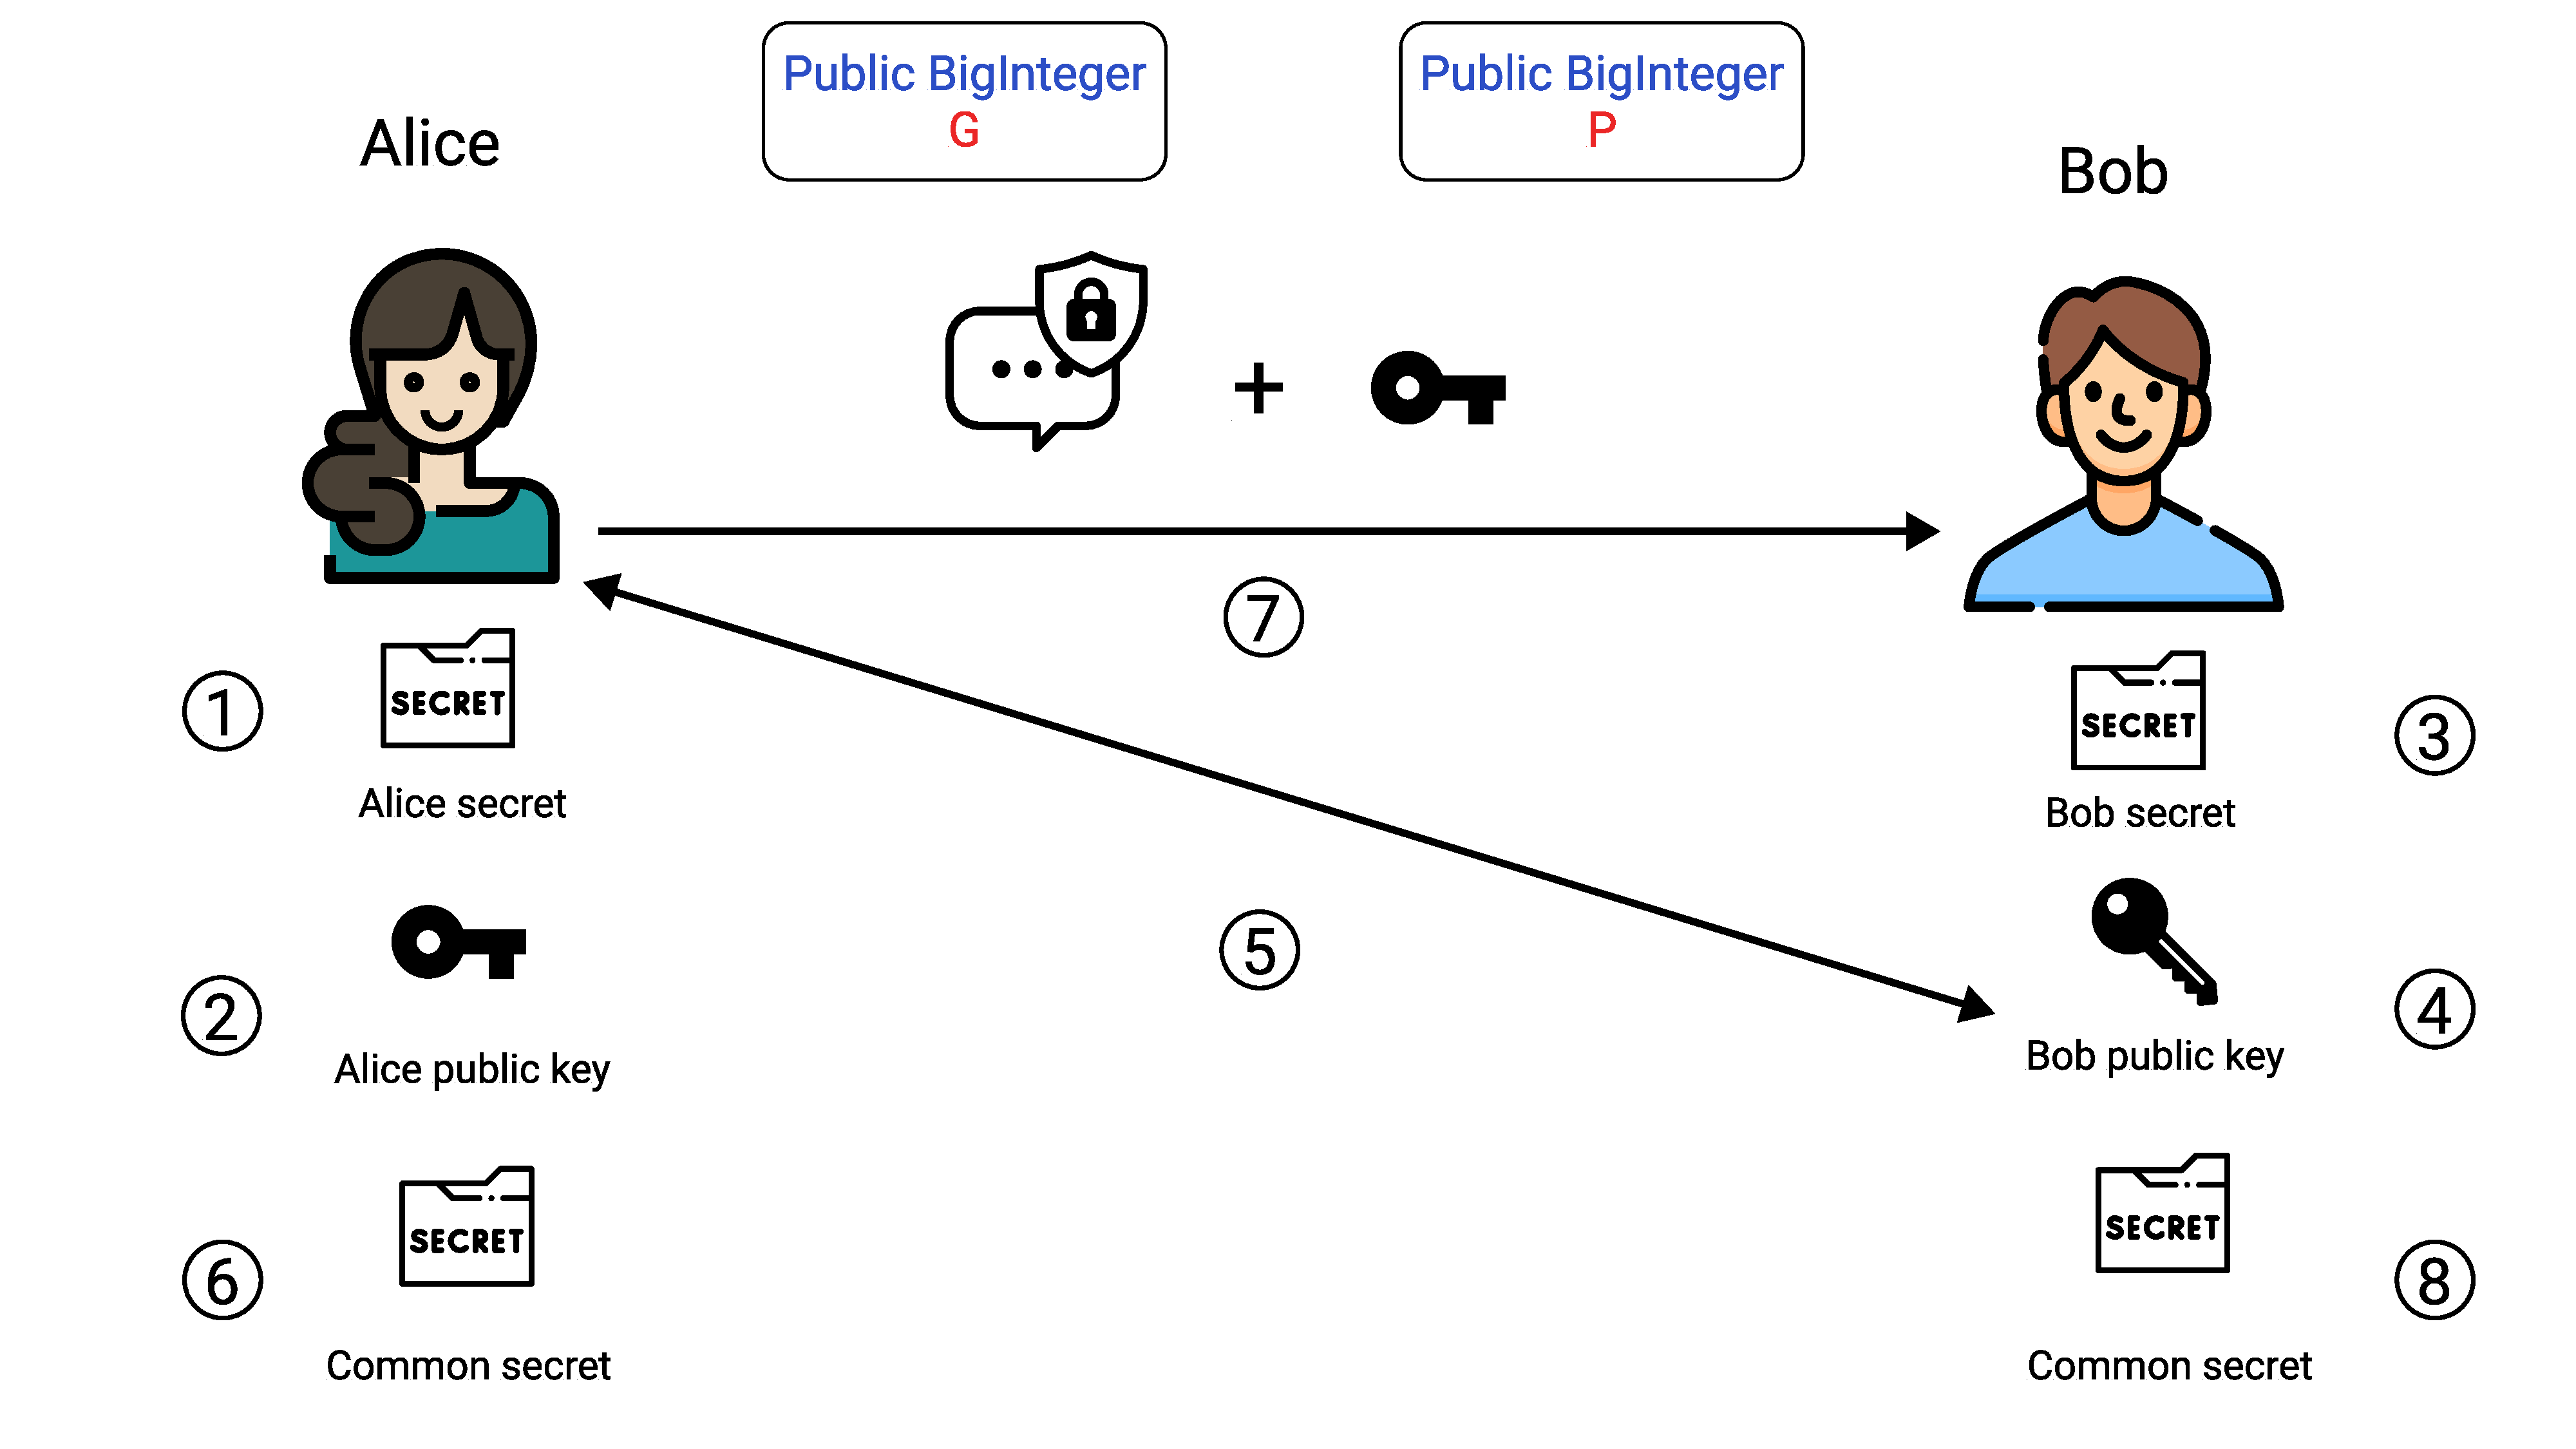
\includegraphics[width=1\textwidth]{Pictures/Key_Exchange}
    \caption{Secret chat encryption concept diagram. Source: }\label{fig:figure7}
\end{figure}
Assume that Alice wants to write a secret message to the Bob.
The secret chat encryption implemented as follows
\begin{enumerate}
    \item Given two public constants: $P, G$.
    \item Alice generates her secret $a$.
    \item Alice generates public key $A$ as $A=G^a \bmod P$ and shares it public.
    \item Bob generates his secret $b$.
    \item Bob generates public key $B$ as $B=G^b \bmod P$ and shares it public.
    \item Alice reads Bob's public key $B$.
    \item Alice calculates Common secret $s$ as $s = B^a \bmod P$.
    \item Alice encrypts message using AES256 algorithm, then sends it to Bob along her public key $A$.
    \item Bob calculates Common secret $s$ as $s = A^b \bmod P$ and decrypts message from Alice.
\end{enumerate}
Although, DH fits the key exchange concerns fine, the secret might be shared via RSA approach as well.
We discuss it in next section.

%\section{RSA Encryption algorithm}\label{sec:rsa-encryption-algorithm2}
%%RSA (Rivest–Shamir–Adleman) is a public-key cryptosystem that is widely used for secure data transmission.
%It is also one of the oldest.
%The acronym RSA comes from the surnames of Ron Rivest, Adi Shamir and Leonard Adleman, who publicly described the
%algorithm in 1977.
%An equivalent system was developed secretly, in 1973 at GCHQ (the British signals intelligence agency), by the
%English mathematician Clifford Cocks.
%That system was declassified in 1997.[1]
%In a public-key cryptosystem, the encryption key is public and distinct from the decryption key, which is kept secret.
%An RSA user creates and publishes a public key based on two large prime numbers, along with an auxiliary value.
%The prime numbers are kept secret.
%Messages can be encrypted by anyone, via the public key, but can only be decoded by someone who knows the prime numbers.
%The security of RSA relies on the practical difficulty of factoring the product of two large prime numbers,
%the "factoring problem".
%Breaking RSA encryption is known as the RSA problem.
%Whether it is as difficult as the factoring problem is an open question.
%There are no published methods to defeat the system if a large enough key is used.
%RSA is a relatively slow algorithm.
%Because of this, it is not commonly used to directly encrypt user data.
%More often, RSA is used to transmit shared keys for symmetric key cryptography, which are then used for bulk
%encryption-decryption.
The RSA algorithm is named after Ron Rivest, Adi Shamir and Len Adleman, who invented it in 1977 [\cite{rivest1978method}].
The basic technique was first discovered in 1973 by Clifford Cocks [\cite{cocks1973note}] of CESG (part of the British GCHQ)
but this was a secret until 1997.
The patent taken out by RSA Labs has expired.

Historically, the process of encryption is considered to be symmetric one.
That means that prior the communication, the sides conclude on the common key to be used in encryption.
This process is similar to the first sharing keys and only after that the locked chest with the message.
Such approach is highly cost since it requires to share the defined keys between each actor if the number of actors
is greater than 2.
Much more simpler is to think about secured communication channel that in terms of asymmetric encryption.
The real life example would be if Alice shares with all actors an opened lock having key.
So that Bob receives an opened lock, writes letter to Alice, puts letter to the chest, locks this chest with received
from Alice lock.
This way, only Alice will be able to open the chest and to read the letter.
This is an idea of the asymmetric encryption.
However, such a simple from first glance idea requires complex number theory approach.
A concept of opened lock may be interpreted in terms of one-way functions.
One way function -- is a function that is easy to compute on every input, but hard to invert given the image of
a random input.
Thus, it is much simpler to close the lock without key, but very difficult to open lock trying the combinations
of the key.
For instance, the function
\begin{equation*}
    f(m) = m^e \bmod N = C
\end{equation*}
where $e, N$ are public constants is one-awy function,
because it is easy to compute $C$ given $m$, however it is hard to compute $m$ given $C$.
So, assume that Alice defines two positive integer constants $e, N$ and sends it to Bob.
Bob encrypts the secret message $m$ using $f(m)$
\[
    f(m) = m^e \bmod N = C
\]
Then Bob sends encrypted message $C$ to the Alice.
Given $C$ Alice must fetch the Bob's message $m$.
In order to decrypt $C$, Alice has to compute
\[
    C^d \bmod N = m^{ed} \bmod N \equiv m,
\]
where $e$ for encryption and $d$ for decryption.
Now the problem is to define such $d$ that it is hard to the listener to fetch it.
In order to define the secret $d$, Alice chooses two enough big prime numbers: $P, \; Q$, let's say around 150 digits
both.
Then Alice multiplies these two prime numbers in order to get $N$
\[
    N = P \cdot Q
\]
The $N$ is around 300 digits.
Now Alice can share $N$ with anyone, since it takes decades to find its prime factorization by the fundamental problem
of prime factorization.
Next, it is very important to know such a function, which depends on the knowledge of factorization of $N$.
Such function is an Euler's totient function.
Given a number $N$ and its prime factorization $p_1^{e_1}\cdot p_2^{e_2} \cdots p_k^{e_k}$, the Euler's totient function
$\phi(N)$ is defined as
\[
    \phi(N) = (p_1^{e_1} - p_1^{e_1 - 1}) \cdot (p_2^{e_2} - p_2^{e_2 - 1}) \cdots (p_k^{e_k} - p_k^{e_k - 1})
\]
In particular, for positive number $M$ such that its factorization is $p1 \cdot p2$, the $\phi(M)$ is
\[
    \phi(M) = (p_1 -1) \cdot (p_2 - 1)
\]
Euler's theorem relates the modular division and exponent as follows, given number $m$, then
\[
    m^{\phi(N)} = 1 \bmod N
\]
It means that reminder of division $m^{\phi(N)}$ by $N$ is always 1.
By the equality $1^K = 1$
\[
    M^{K \cdot \phi(N)} = 1 \bmod N
\]
If we multiply both parts by $M$, we get
\[
    M \cdot M^{K \cdot \phi(N)} = M^{K \cdot \phi(N) + 1} = M \bmod N
\]
It follows that Alice is able to define the secret $d$ as follows
\begin{gather*}
    e \cdot d = K \cdot \phi(N) + 1\\
    d = \frac{K \cdot \phi(N) + 1}{e}\\
\end{gather*}
The following image demonstrates the concept of RSA approach
\begin{figure}[H]
    \centering
    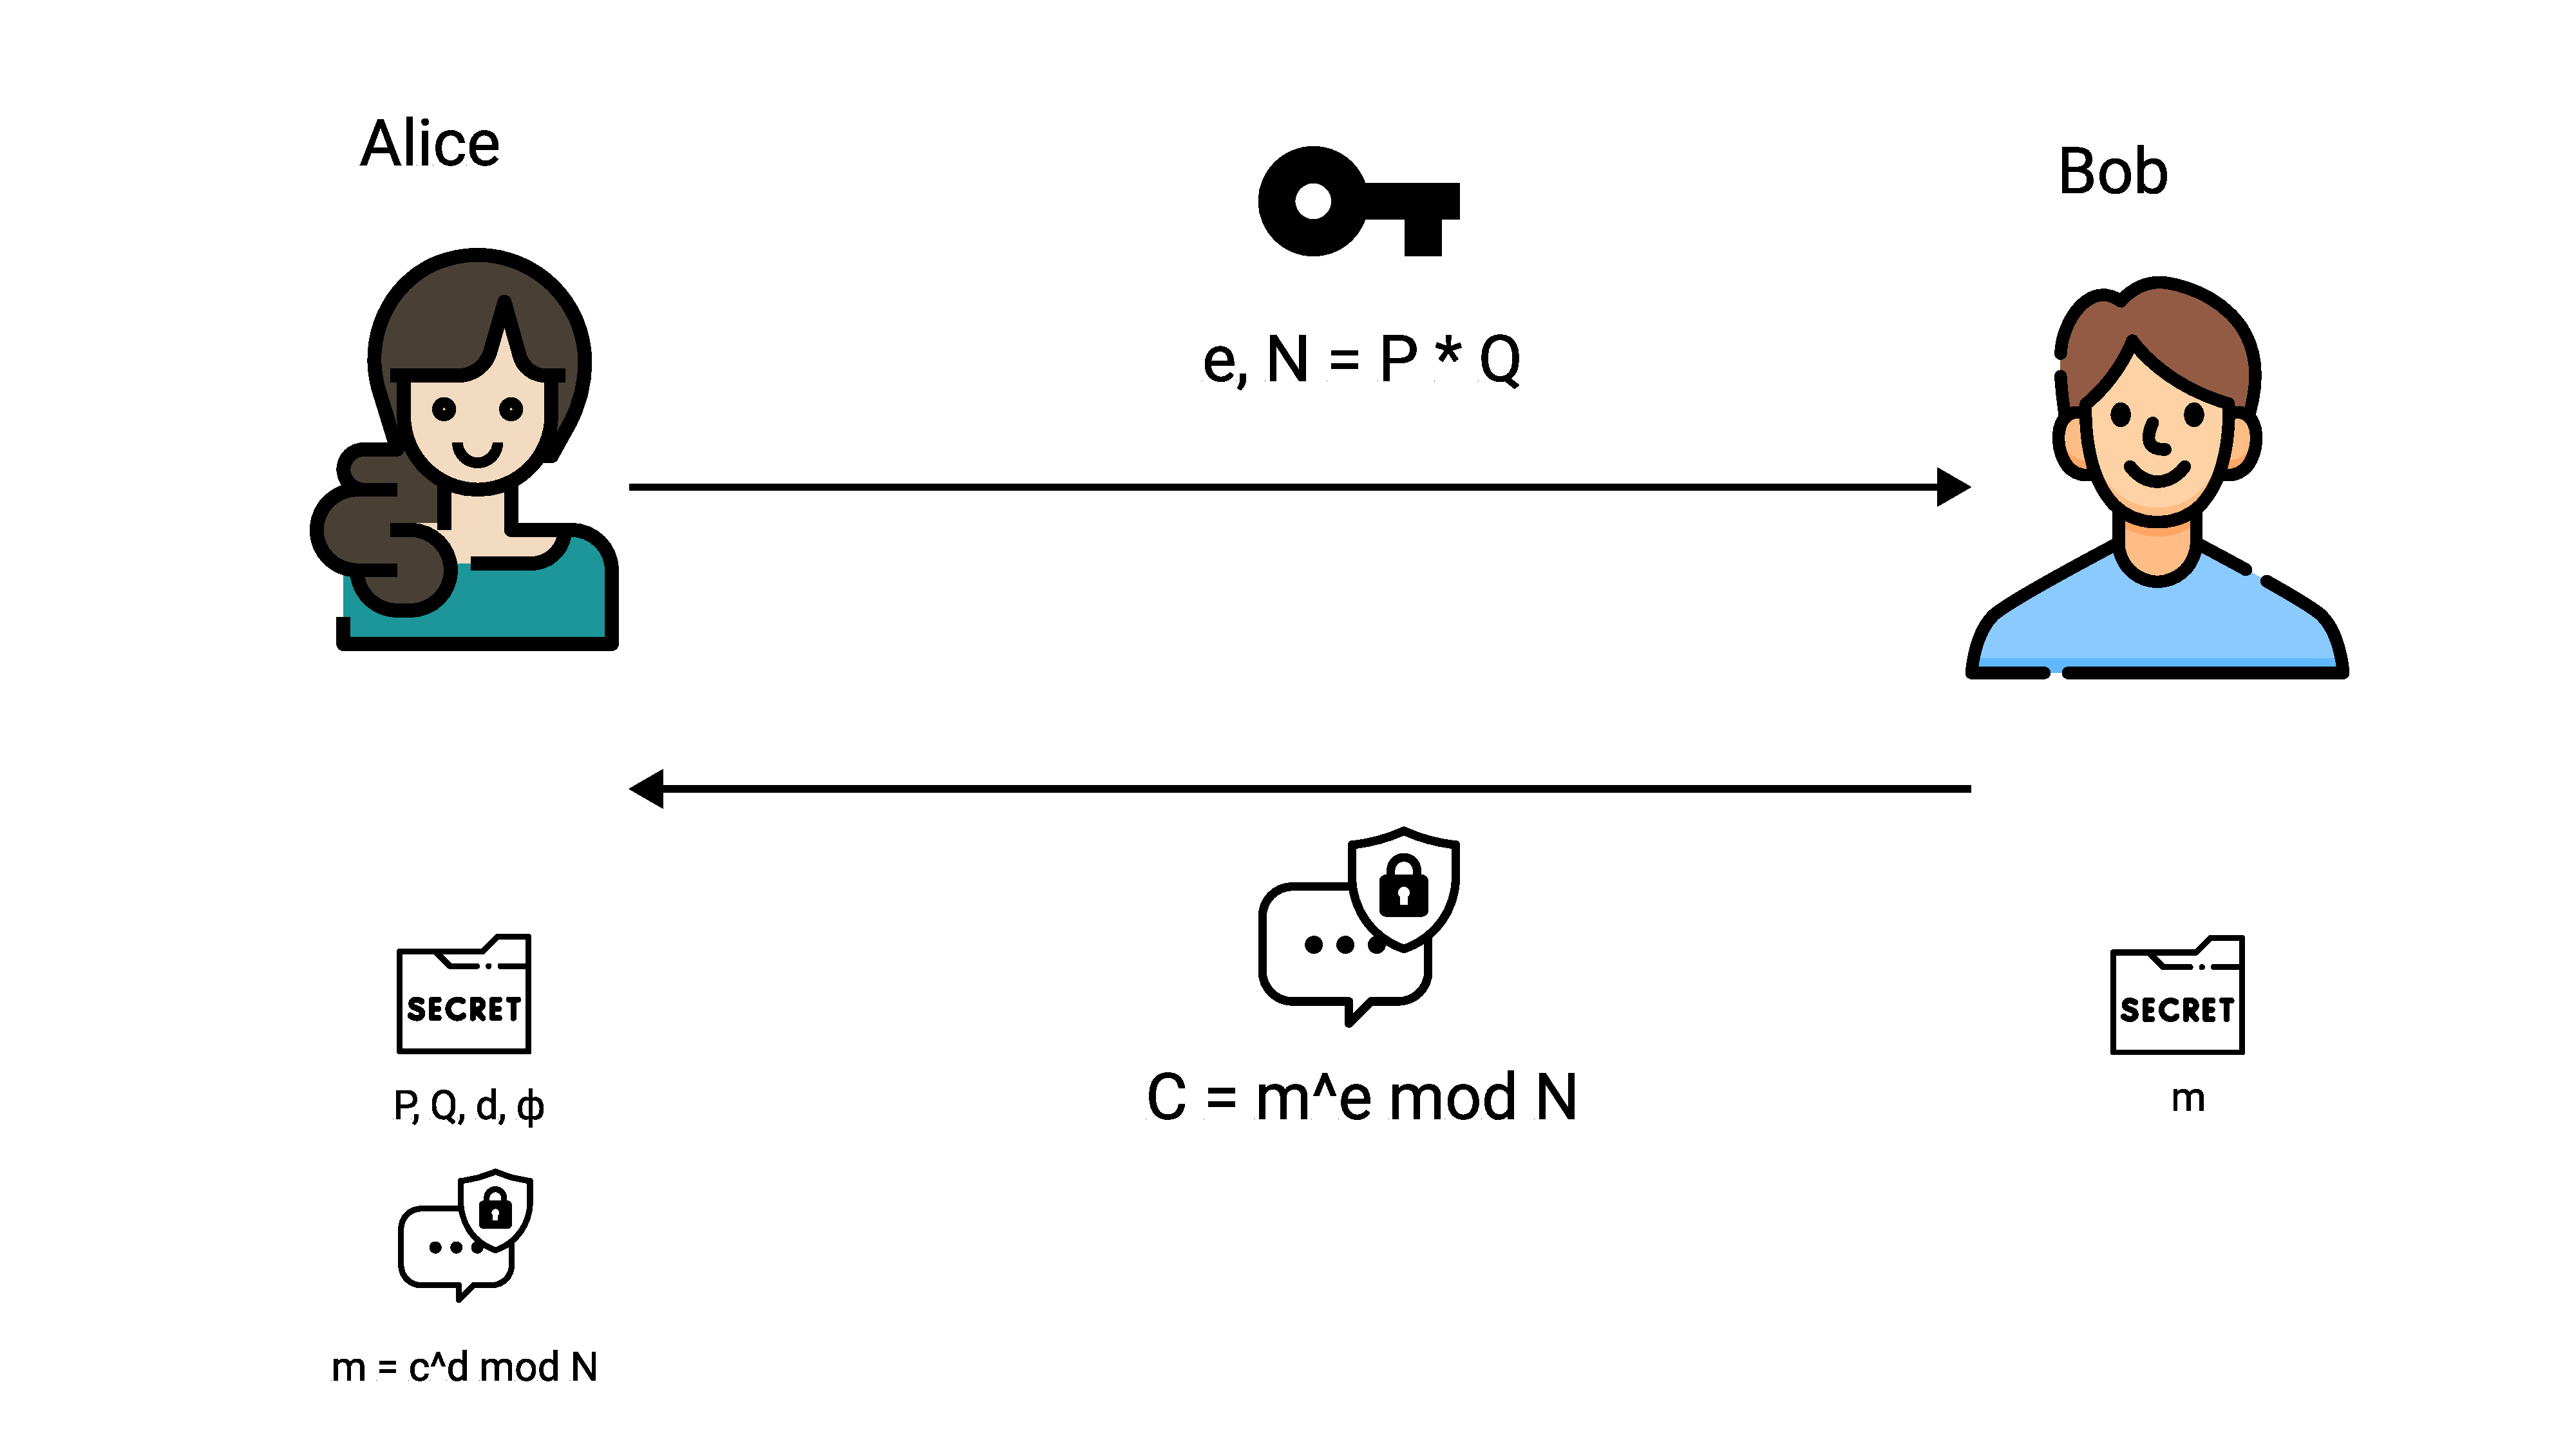
\includegraphics[width=1\textwidth]{Pictures/RSA_diagram}
    \caption{Secret chat encryption concept diagram. Source: }\label{fig:figure8}
\end{figure}
To summarize, the process by the steps is as follows
\begin{itemize}
    \item Alice defines her secrets: $P, \; Q, \; \phi, d$.
    \item Alice defines public constants $e, N = P \cdot Q$ and shares them with Bob.
    \item Bob defines the message $m$, encrypts it as $C = m^{e} \bmod N$.
    \item Bob sends $C$ to Alice.
    \item Alice decrypts $C$ using her secret $d$, so she gets $m$
    \[
        m = C^d \bmod N
    \]
\end{itemize}
Security of the RSA approach is based on the complexity of fundamental problem of prime factorization,
which takes decades to solve having enough large number.
    \chapter{User Interface}\label{ch:user-interface}

Here to be filled sections with screenshots, after functional requirements updated.
    \chapter{Conclusions}\label{ch:conclusions}

%----------------------------------------------------------------------------------------
%	BIBLIOGRAPHY
%----------------------------------------------------------------------------------------

    \printbibliography[heading=bibintoc]

%----------------------------------------------------------------------------------------

%----------------------------------------------------------------------------------------
%	THESIS CONTENT - APPENDICES
%----------------------------------------------------------------------------------------

    \appendix % Cue to tell LaTeX that the following "chapters" are Appendices

% Include the appendices of the thesis as separate files from the Appendices folder
% Uncomment the lines as you write the Appendices

    %\chapter{Web API Documentation}\label{ch:web-api-documentation}


\section{Auth}\label{sec:auth}
\begin{itemize}
    %% Register Endpoint
    \item \textbf{Endpoint}: /api/auth/register
    \begin{itemize}
        \item \textbf{Description}: Registers user in a messenger
        \item \textbf{Request type}: POST
        \item \textbf{Request body}:
        \begin{spverbatim}
        {
            "phoneNumber": "string",
            "email": "string",
            "displayName": "string",
            "password": "string",
            "verificationMethod": number,
            "termsAccepted": boolean
        }
        \end{spverbatim}
        \item  \textbf{Response example}:
        \begin{itemize}
            \item \textbf{200 Success}:
            \begin{spverbatim}
            {
                "message": "SUCCESS",
                "success": true
            }
            \end{spverbatim}
            \item \textbf{400 Bad Request}:
            \begin{spverbatim}
            {
                "errorMessage": "string",
                "errorDetails": "string",
                "statusCode": 0,
                "success": true
            }
            \end{spverbatim}
            \item \textbf{409 Conflict}:
            \begin{spverbatim}
            {
                "errorMessage": "string",
                "errorDetails": "string",
                "statusCode": 0,
                "success": true
            }
            \end{spverbatim}
        \end{itemize}
        \item \textbf{Response messages}:
        \begin{enumerate}
            \item Success.
            \item User already registered.
            \item Weak password.
            \item Invalid email.
            \item Invalid verification method.
            \item Invalid display name.
            \item Phone occupied.
        \end{enumerate}
    \end{itemize}
    %% Register Endpoint

    %% Verify Email Endpoint
    \item \textbf{Endpoint}: api/auth/verify-email
    \begin{itemize}
        \item \textbf{Description}: Sends verification request.
        User receives confirmation link via email.
        \item \textbf{Request type}: POST
        \item \textbf{Request body}:
        \begin{spverbatim}
        {
            "email": "string",
            "userId": "string"
        }
        \end{spverbatim}
        \item  \textbf{Response example}:
        \begin{itemize}
            \item \textbf{200 Success}:
            \begin{spverbatim}
            {
                "message": "SUCCESS",
                "success": true
            }
            \end{spverbatim}
            \item \textbf{400 Bad Request}:
            \begin{spverbatim}
            {
                "errorMessage": "string",
                "errorDetails": "string",
                "statusCode": 0,
                "success": true
            }
            \end{spverbatim}
            \item \textbf{409 Conflict}:
            \begin{spverbatim}
            {
                "errorMessage": "string",
                "errorDetails": "string",
                "statusCode": 0,
                "success": true
            }
            \end{spverbatim}
        \end{itemize}
        \item \textbf{Response messages}:
        \begin{enumerate}
            \item Success.
            \item User already registered.
            \item Weak password.
            \item Invalid email.
            \item Invalid verification method.
            \item Invalid display name.
            \item Phone occupied.
        \end{enumerate}
        \item \textbf{Response messages}:
        \begin{enumerate}
            \item Success.
            \item Invalid user id.
            \item Email already verified.
        \end{enumerate}
    \end{itemize}
    %% Verify Email Endpoint

    %% Verify Phone Endpoint
    \item \textbf{Endpoint}: api/auth/verify-phone
    \begin{itemize}
        \item \textbf{Description}: Sends SMS to user phone.
        \item \textbf{Request type}: POST
        \item \textbf{Request body}:
        \begin{spverbatim}
        {
            "confirmationCode": 0,
            "userId": "string"
        }
        \end{spverbatim}
        \item  \textbf{Response example}:
        \begin{itemize}
            \item \textbf{200 Success}:
            \begin{spverbatim}
            {
                "message": "SUCCESS",
                "success": true
            }
            \end{spverbatim}
            \item \textbf{400 Bad Request}:
            \begin{spverbatim}
            {
                "errorMessage": "string",
                "errorDetails": "string",
                "statusCode": 0,
                "success": true
            }
            \end{spverbatim}
            \item \textbf{409 Conflict}:
            \begin{spverbatim}
            {
                "errorMessage": "string",
                "errorDetails": "string",
                "statusCode": 0,
                "success": true
            }
            \end{spverbatim}
        \end{itemize}
        \item \textbf{Response messages}:
        \begin{enumerate}
            \item Success.
            \item Invalid or expired.
            \item Phone already verified
        \end{enumerate}
    \end{itemize}
    %% Verify Phone Endpoint

    %% Login Endpoint
    \item \textbf{Endpoint}: api/auth/login
    \begin{itemize}
        \item \textbf{Description}: Performs login to the messenger.
        \item \textbf{Request type}: POST
        \item \textbf{Request body}:
        \begin{spverbatim}
        {
            "email": "string",
            "password": "string"
        }
        \end{spverbatim}
        \item \textbf{Response example}:
        \begin{itemize}
            \item \textbf{200 Success}:
            \begin{spverbatim}
            {
                "refreshTokenId": "string",
                "accessToken": "string",
                "message": "string",
                "success": true
            }
            \end{spverbatim}
            \item \textbf{400 Bad Request}:

            \begin{spverbatim}
            {
                "errorMessage": "string",
                "errorDetails": "string",
                "statusCode": 0,
                "success": true
            }
            \end{spverbatim}
            \item \textbf{409 Conflict}:
            \begin{spverbatim}
            {
                "errorMessage": "string",
                "errorDetails": "string",
                "statusCode": 0,
                "success": true
            }
            \end{spverbatim}
        \end{itemize}
        \item \textbf{Response messages}:
        \begin{enumerate}
            \item Success.
            \item Invalid credentials.
        \end{enumerate}
    \end{itemize}
    %% Login Endpoint


    %% Refresh Token Endpoint
    \item \textbf{Endpoint}: api/auth/refresh-token
    \begin{itemize}
        \item \textbf{Description}: Refreshes user's existing refresh token and access token.
        \item \textbf{Request type}: POST
        \item \textbf{Request body}:
        \begin{spverbatim}
        {
            "refreshTokenId": "string"
        }
        \end{spverbatim}
        \item  \textbf{Response example}:
        \begin{itemize}
            \item \textbf{200 Success}:
            \begin{spverbatim}
            {
                "refreshTokenId": "string",
                "accessToken": "string",
                "message": "string",
                "success": true
            }
            \end{spverbatim}
            \item \textbf{400 Bad Request}:
            \begin{spverbatim}
            {
                "errorMessage": "string",
                "errorDetails": "string",
                "statusCode": 0,
                "success": true
            }
            \end{spverbatim}
            \item \textbf{409 Conflict}:
            \begin{spverbatim}
            {
                "errorMessage": "string",
                "errorDetails": "string",
                "statusCode": 0,
                "success": true
            }
            \end{spverbatim}
        \end{itemize}
        \item \textbf{Response messages}:
        \begin{enumerate}
            \item Success.
            \item Invalid or empty refresh token.
        \end{enumerate}
    \end{itemize}
    %% Refresh Token Endpoint

    %% Logout Endpoint
    \item \textbf{Endpoint}: api/auth/logout
    \begin{itemize}
        \item \textbf{Description}: Logs out from current device.
        \item \textbf{Request type}: POST
        \item \textbf{Request body}:
        \begin{spverbatim}
        {
            "refreshTokenId": "string"
        }
        \end{spverbatim}
        \item \textbf{Response example}:
        \begin{itemize}
            \item \textbf{200 Success}:
            \begin{spverbatim}
            {
                "message": "SUCCESS",
                "success": true
            }
            \end{spverbatim}
            \item \textbf{400 Bad Request}:
            \begin{spverbatim}
            {
                "errorMessage": "string",
                "errorDetails": "string",
                "statusCode": 0,
                "success": true
            }
            \end{spverbatim}
            \item \textbf{409 Conflict}:
            \begin{spverbatim}
            {
                "errorMessage": "string",
                "errorDetails": "string",
                "statusCode": 0,
                "success": true
            }
            \end{spverbatim}
        \end{itemize}
        \item \textbf{Response messages}:
        \begin{enumerate}
            \item Success.
            \item User not found.
            \item Invalid or empty refresh token.
        \end{enumerate}
    \end{itemize}
    %% Logout Endpoint

    %% Logout All Endpoint
    \item \textbf{Endpoint}: api/auth/logout-all
    \begin{itemize}
        \item \textbf{Description}: Logs out from all devices.
        \item \textbf{Request type}: POST
        \item \textbf{Request body}:
        \begin{spverbatim}
        {
            "refreshTokenId": "string"
        }
        \end{spverbatim}
        \item  \textbf{Response example}:
        \begin{itemize}
            \item \textbf{200 Success}:
            \begin{spverbatim}
            {
                "message": "SUCCESS",
                "success": true
            }
            \end{spverbatim}
            \item \textbf{400 Bad Request}:
            \begin{spverbatim}
            {
                "errorMessage": "string",
                "errorDetails": "string",
                "statusCode": 0,
                "success": true
            }
            \end{spverbatim}
            \item \textbf{409 Conflict}:
            \begin{spverbatim}
            {
                "errorMessage": "string",
                "errorDetails": "string",
                "statusCode": 0,
                "success": true
            }
            \end{spverbatim}
        \end{itemize}
    \end{itemize}
    %% Logout All Endpoint

\end{itemize}


\section{Chats}\label{sec:chats}
\begin{itemize}
    %% Get Chats Endpoint
    \item \textbf{Endpoint}: api/chats
    \begin{itemize}
        \item \textbf{Description}: Returns list of all user's chats.
        \item \textbf{Request type}: GET
        \item \textbf{Response example}:
        \textbf{200 Success}:
        \begin{spverbatim}
        {
            "chats": [
                {
                "chatId": "string",
                "title": "string",
                "image": "string",
                "lastMessageAuthor": "string",
                "lastMessage": "string",
                "lastMessageAt": "string",
                "membersCount": 0,
                "isMember": true
            }
            ],
            "message": "string",
            "success": true
        }
        \end{spverbatim}
        \textbf{400 Bad Request}:
        \begin{spverbatim}
        {
            "errorMessage": "string",
            "errorDetails": "string",
            "statusCode": 0,
            "success": true
        }
        \end{spverbatim}
        \textbf{409 Conflict}:
        \begin{spverbatim}
        {
            "errorMessage": "string",
            "errorDetails": "string",
            "statusCode": 0,
            "success": true
        }
        \end{spverbatim}
        \item \textbf{Response messages}:
        \begin{enumerate}
            \item Success.
            \item User not found.
        \end{enumerate}
    \end{itemize}
    %% Get Chats Endpoint

    %% Create Group Endpoint
    \item \textbf{Endpoint}: api/chats/group
    \begin{itemize}
        \item \textbf{Description}: Creates new group of specified type.
        \item \textbf{Request type}: POST
        \item \textbf{Request body}:
        \begin{spverbatim}
        {
            "groupType": 1
            "groupTitle": "string"
        }
        \end{spverbatim}
        \item \textbf{Chat types}:
        \begin{enumerate}
            \item DirectChat -- Chat between two people
            \item PrivateChannel -- Channel that can be joined only via invite link from owner or one of the members
            \item PublicChannel -- Channel that can be joined and messaged by anyone, unless person is not in blacklist
            \item ReadOnlyChannel -- Channel that can be joined by anyone, but any member except owner or moderator cannot send messages there
        \end{enumerate}
        \item \textbf{Response example}:
        \textbf{200 Success}:
        \begin{spverbatim}
        {
            "chatId": "string",
            "message": "string",
            "success": true
        }
        \end{spverbatim}
        \textbf{400 Bad Request}:
        \begin{spverbatim}
        {
            "errorMessage": "string",
            "errorDetails": "string",
            "statusCode": 0,
            "success": true
        }
        \end{spverbatim}
        \textbf{409 Conflict}:
        \begin{spverbatim}
        {
            "errorMessage": "string",
            "errorDetails": "string",
            "statusCode": 0,
            "success": true
        }
        \end{spverbatim}
        \item \textbf{Response messages}:
        \begin{enumerate}
            \item Success.
            \item User not found.
        \end{enumerate}
    \end{itemize}
    %% Create Group Endpoint

    %% Create Direct Chat Endpoint
    \item \textbf{Endpoint}: api/chats/direct-chat
    \begin{itemize}
        \item \textbf{Description}: Creates new group of specified type.
        \item \textbf{Request type}: POST
        \item \textbf{Request body}:
        \begin{spverbatim}
        {
            "partnerId": "string"
        }
        \end{spverbatim}
        \item \textbf{Response example}:
        \textbf{200 Success}:
        \begin{spverbatim}
        {
            "chatId": "string",
            "message": "string",
            "success": true
        }
        \end{spverbatim}
        \textbf{400 Bad Request}:
        \begin{spverbatim}
        {
            "errorMessage": "string",
            "errorDetails": "string",
            "statusCode": 0,
            "success": true
        }
        \end{spverbatim}
        \textbf{409 Conflict}:
        \begin{spverbatim}
        {
            "errorMessage": "string",
            "errorDetails": "string",
            "statusCode": 0,
            "success": true
        }
        \end{spverbatim}
        \item \textbf{Response messages}:
        \begin{enumerate}
            \item Success.
            \item User not found.
        \end{enumerate}
    \end{itemize}
    %% Create Direct Chat Endpoint

    %% Group Join Endpoint
    \item \textbf{Endpoint}: api/chats/group/join/\{chatId\}
    \begin{itemize}
        \item \textbf{Description}: Creates new group of specified type.
        \item \textbf{Request type}: POST
        \item \textbf{Request example}:
        \begin{spverbatim}
        {
            "chatId": "string"
        }
        \end{spverbatim}
        \item \textbf{Response example}:
        \textbf{200 Success}:
        \begin{spverbatim}
        {
            "chatId": "string",
            "message": "string",
            "success": true
        }
        \end{spverbatim}
        \textbf{400 Bad Request}:
        \begin{spverbatim}
        {
            "errorMessage": "string",
            "errorDetails": "string",
            "statusCode": 0,
            "success": true
        }
        \end{spverbatim}
        \textbf{409 Conflict}:
        \begin{spverbatim}
        {
            "errorMessage": "string",
            "errorDetails": "string",
            "statusCode": 0,
            "success": true
        }
        \end{spverbatim}
        \item \textbf{Response messages}:
        \begin{enumerate}
            \item Success.
            \item Group not found.
        \end{enumerate}
    \end{itemize}
    %% Group Join Endpoint

    %% Search Chat Endpoint
    \item \textbf{Endpoint}: api/chats/search
    \begin{itemize}
        \item \textbf{Description}: Searches chats by display name.
        \item \textbf{Request type}: GET
        \item \textbf{Parameters}:
        \begin{enumerate}
            \item displayName (required)
        \end{enumerate}
        \item \textbf{Response example}:
        \textbf{200 Success}:
        \begin{spverbatim}
        {
            "chats": [
                {
                "chatId": "string",
                "title": "string",
                "image": "string",
                "lastMessageAuthor": "string",
                "lastMessage": "string",
                "lastMessageAt": "string",
                "membersCount": 0,
                "isMember": true
            }
            ],
            "message": "string",
            "success": true
        }
        \end{spverbatim}
        \textbf{400 Bad Request}:
        \begin{spverbatim}
        {
            "errorMessage": "string",
            "errorDetails": "string",
            "statusCode": 0,
            "success": true
        }
        \end{spverbatim}
        \textbf{409 Conflict}:
        \begin{spverbatim}
        {
            "errorMessage": "string",
            "errorDetails": "string",
            "statusCode": 0,
            "success": true
        }
        \end{spverbatim}
        \item \textbf{Response messages}:
        \begin{enumerate}
            \item Success.
            \item Unauthorized.
        \end{enumerate}
    \end{itemize}
    %% Search Chat Endpoint

\end{itemize}


\section{Messages}\label{sec:messages}
\begin{itemize}
    %% Get Chat Messages Endpoint
    \item \textbf{Endpoint}: /api/messages/\{chatId\}
    \begin{itemize}
        \item \textbf{Description}: Returns chat including messages by chat id.
        \item \textbf{Request type}: GET
        \item \textbf{Parameters}:
        \begin{enumerate}
            \item Chat id (required).
        \end{enumerate}
        \item \textbf{Response example}:
        \begin{itemize}
            \item \textbf{200 Success}:
            \begin{spverbatim}
            {
                "messages": [
                    {
                        "userDisplayName": "string",
                        "messageText": "string",
                        "sentAt": "string",
                        "editedAt": "string",
                        "self": true
                    }
                ],
                "message": "string",
                "success": true
            }
            \end{spverbatim}
            \item \textbf{400 Bad Request}:
            \begin{spverbatim}
            {
                "errorMessage": "string",
                "errorDetails": "string",
                "statusCode": 0,
                "success": true
            }
            \end{spverbatim}
            \item \textbf{409 Conflict}:
            \begin{spverbatim}
            {
                "errorMessage": "string",
                "errorDetails": "string",
                "statusCode": 0,
                "success": true
            }
            \end{spverbatim}
        \end{itemize}
        \item \textbf{Response messages}:
        \begin{enumerate}
            \item Success.
            \item User not found.
        \end{enumerate}
    \end{itemize}
    %% Get Chat Messages Endpoint

    %% Send Message Endpoint
    \item \textbf{Endpoint}: /api/messages
    \begin{itemize}
        \item \textbf{Description}: Sends message to particular chat
        \item \textbf{Request type}: POST
        \item \textbf{Request body}:
        \begin{spverbatim}
        {
            "messageId": "string",
            "message": "string",
            "success": true
        }
        \end{spverbatim}
        \item \textbf{Response example}:
        \begin{itemize}
            \item \textbf{200 Success}:
            \begin{spverbatim}
            {
                "message": "SUCCESS",
                "success": true
            }
            \end{spverbatim}
            \item \textbf{400 Bad Request}:
            \begin{spverbatim}
            {
                "errorMessage": "string",
                "errorDetails": "string",
                "statusCode": 0,
                "success": true
            }
            \end{spverbatim}
            \item \textbf{409 Conflict}:
            \begin{spverbatim}
            {
                "errorMessage": "string",
                "errorDetails": "string",
                "statusCode": 0,
                "success": true
            }
            \end{spverbatim}
        \end{itemize}
        \item \textbf{Response messages}:
        \begin{enumerate}
            \item Success.
            \item User not found.
        \end{enumerate}
    \end{itemize}
    %% Send Message Endpoint

    %% Edit Message Endpoint
    \item \textbf{Endpoint}: /api/messages
    \begin{itemize}
        \item \textbf{Description}: Updates particular message
        \item \textbf{Request type}: PUT
        \item \textbf{Request body}:
        \begin{spverbatim}
        {
            "messageId": "string",
            "modifiedText": "string"
        }
        \end{spverbatim}
        \item \textbf{Response example}:
        \begin{itemize}
            \item \textbf{200 Success}:
            \begin{spverbatim}
            {
                "message": "SUCCESS",
                "success": true
            }
            \end{spverbatim}
            \item \textbf{400 Bad Request}:
            \begin{spverbatim}
            {
                "errorMessage": "string",
                "errorDetails": "string",
                "statusCode": 0,
                "success": true
            }
            \end{spverbatim}
            \item \textbf{409 Conflict}:
            \begin{spverbatim}
            {
                "errorMessage": "string",
                "errorDetails": "string",
                "statusCode": 0,
                "success": true
            }
            \end{spverbatim}
        \end{itemize}
        \item \textbf{Response messages}:
        \begin{enumerate}
            \item Success.
            \item User not found.
        \end{enumerate}
    \end{itemize}
    %% Edit Message Endpoint

    %% Delete Message Endpoint
    \item \textbf{Endpoint}: /api/messages
    \begin{itemize}
        \item \textbf{Description}: Deletes particular message
        \item \textbf{Request type}: DELETE
        \item \textbf{Request body}:
        \begin{spverbatim}
        {
            "messageId": "string"
        }
        \end{spverbatim}
        \item \textbf{Response example}:
        \begin{itemize}
            \item \textbf{200 Success}:
            \begin{spverbatim}
            {
                "message": "SUCCESS",
                "success": true
            }
            \end{spverbatim}
            \item \textbf{400 Bad Request}:
            \begin{spverbatim}
            {
                "errorMessage": "string",
                "errorDetails": "string",
                "statusCode": 0,
                "success": true
            }
            \end{spverbatim}
            \item \textbf{409 Conflict}:
            \begin{spverbatim}
            {
                "errorMessage": "string",
                "errorDetails": "string",
                "statusCode": 0,
                "success": true
            }
            \end{spverbatim}
        \end{itemize}
        \item \textbf{Response messages}:
        \begin{enumerate}
            \item Success.
            \item User not found.
        \end{enumerate}
    \end{itemize}
    %% Delete Message Endpoint
\end{itemize}


\section{User}\label{sec:user}
\begin{itemize}
    %% Get User Endpoint
    \item \textbf{Endpoint}: /api/users/\{userId\}
    \begin{itemize}
        \item \textbf{Description}: Returns information about particular user by user ID
        \item \textbf{Request type}: GET
        \item \textbf{Parameters}:
        \begin{enumerate}
            \item User ID (required).
        \end{enumerate}
        \item \textbf{Response example}:
        \textbf{200 Success}:
        \begin{spverbatim}
        {
            "message": "string",
            "success": true
        }
        \end{spverbatim}
        \textbf{400 Bad Request}:
        \begin{spverbatim}
        {
            "errorMessage": "string",
            "errorDetails": "string",
            "statusCode": 0,
            "success": true
        }
        \end{spverbatim}
        \textbf{409 Conflict}:
        \begin{spverbatim}
        {
            "errorMessage": "string",
            "errorDetails": "string",
            "statusCode": 0,
            "success": true
        }
        \end{spverbatim}
        \item \textbf{Response messages}:
        \begin{enumerate}
            \item Success.
            \item User not found.
        \end{enumerate}
    \end{itemize}
    %% Get User Endpoint
    %% Get Current User Endpoint
    \item \textbf{Endpoint}: /api/users
    \begin{itemize}
        \item \textbf{Description}: Returns information about current user logged in system
        \item \textbf{Request type}: GET
        \item \textbf{Response example}:
        \textbf{200 Success}:
        \begin{spverbatim}
        {
            "user": {
            "username": "string",
            "displayName": "string",
            "bio": "string",
            "image": "string"
        },
            "message": "string",
            "success": true
        }
        \end{spverbatim}
        \textbf{400 Bad Request}:
        \begin{spverbatim}
        {
            "errorMessage": "string",
            "errorDetails": "string",
            "statusCode": 0,
            "success": true
        }
        \end{spverbatim}
        \textbf{409 Conflict}:
        \begin{spverbatim}
        {
            "errorMessage": "string",
            "errorDetails": "string",
            "statusCode": 0,
            "success": true
        }
        \end{spverbatim}
        \item \textbf{Response messages}:
        \begin{enumerate}
            \item Success.
            \item User not found.
        \end{enumerate}
    \end{itemize}
    %% Get Loged User Endpoint
    %% Search User Endpoint
    \item \textbf{Endpoint}: /api/users/search
    \begin{itemize}
        \item \textbf{Description}: Searches user by display name
        \item \textbf{Request type}: GET
        \item \textbf{Parameters}:
        \begin{enumerate}
            \item displayName (required)
        \end{enumerate}
        \item \textbf{Response example}:
        \textbf{200 Success}:
        \begin{spverbatim}
        {
            "user": {
            "username": "string",
            "displayName": "string",
            "bio": "string",
            "image": "string"
        },
            "message": "string",
            "success": true
        }
        \end{spverbatim}
        \textbf{400 Bad Request}:
        \begin{spverbatim}
        {
            "errorMessage": "string",
            "errorDetails": "string",
            "statusCode": 0,
            "success": true
        }
        \end{spverbatim}
        \textbf{409 Conflict}:
        \begin{spverbatim}
        {
            "errorMessage": "string",
            "errorDetails": "string",
            "statusCode": 0,
            "success": true
        }
        \end{spverbatim}
        \item \textbf{Response messages}:
        \begin{enumerate}
            \item Success.
            \item User not found.
        \end{enumerate}
    \end{itemize}
    %% Search User Endpoint
\end{itemize}


\section{Contacts}\label{sec:contacts}
\begin{itemize}
    %% Add Contact Endpoint
    \item \textbf{Endpoint}: /api/contacts
    \begin{itemize}
        \item \textbf{Description}: Adds new contact
        \item \textbf{Request type}: POST
        \item \textbf{Request body}:
        \begin{spverbatim}
        {
            "contactId": "string"
        }
        \end{spverbatim}
        \item \textbf{Response example}:
        \textbf{200 Success}:
        \begin{spverbatim}
        {
            "message": "string",
            "success": true
        }
        \end{spverbatim}
        \textbf{400 Bad Request}:
        \begin{spverbatim}
        {
            "errorMessage": "string",
            "errorDetails": "string",
            "statusCode": 0,
            "success": true
        }
        \end{spverbatim}
        \textbf{409 Conflict}:
        \begin{spverbatim}
        {
            "errorMessage": "string",
            "errorDetails": "string",
            "statusCode": 0,
            "success": true
        }
        \end{spverbatim}
        \item \textbf{Response messages}:
        \begin{enumerate}
            \item Success.
            \item User not found.
        \end{enumerate}
    \end{itemize}
    %% Add Contact Endpoint
    %% Get Contacts Endpoint
    \item \textbf{Endpoint}: /api/contacts
    \begin{itemize}
        \item \textbf{Description}: Returns list of all user's contacts
        \item \textbf{Request type}: GET
        \item \textbf{Response example}:
        \textbf{200 Success}:
        \begin{spverbatim}
        {
            "contacts": [
                {
                "username": "string",
                "displayName": "string",
                "bio": "string",
                "image": "string"
            }
            ],
            "message": "string",
            "success": true
        }
        \end{spverbatim}
        \textbf{400 Bad Request}:
        \begin{spverbatim}
        {
            "errorMessage": "string",
            "errorDetails": "string",
            "statusCode": 0,
            "success": true
        }
        \end{spverbatim}
        \textbf{409 Conflict}:
        \begin{spverbatim}
        {
            "errorMessage": "string",
            "errorDetails": "string",
            "statusCode": 0,
            "success": true
        }
        \end{spverbatim}
        \item \textbf{Response messages}:
        \begin{enumerate}
            \item Success.
            \item User not found.
        \end{enumerate}
    \end{itemize}
    %% Get Contacts Endpoint
\end{itemize}


\section{User Information}\label{sec:user-information}
\begin{itemize}
    %% Update User Info Endpoint
    \item \textbf{Endpoint}: /api/contacts
    \begin{itemize}
        \item \textbf{Description}: Updates current user information
        \item \textbf{Request type}: PUT
        \item \textbf{Request body}:
        \begin{spverbatim}
        {
            "firstName": "string",
            "lastName": "string",
            "birthDay": "timestamp",
            "website": "string",
            "address": "string",
            "facebook": "string",
            "twitter": "string",
            "instagram": "string",
            "linkedIn": "string",
            "profilePicture": "string"
        }
        \end{spverbatim}
        \item \textbf{Response example}:
        \begin{itemize}
            \item \textbf{200 Success}:
            \begin{spverbatim}
            {
                "message": "string",
                "success": true
            }
            \end{spverbatim}
            \item \textbf{400 Bad Request}:
            \begin{spverbatim}
            {
                "errorMessage": "string",
                "errorDetails": "string",
                "statusCode": 0,
                "success": true
            }
            \end{spverbatim}
            \item \textbf{409 Conflict}:
            \begin{spverbatim}
            {
                "errorMessage": "string",
                "errorDetails": "string",
                "statusCode": 0,
                "success": true
            }
            \end{spverbatim}
        \end{itemize}
        \item \textbf{Response messages}:
        \begin{enumerate}
            \item Success.
            \item User not found.
        \end{enumerate}
    \end{itemize}
    %% Update User Info Endpoint
\end{itemize}
    \chapter{RSA Algorithm comments}\label{ch:rsa-algorithm-comments}
One way function -- is a function that is easy to compute on every input, but hard to invert given the image of a random input.
The function
\[
    m^e \bmod N \equiv C
\]
where $e, N$ are public constants is one-awy function,
because it is easy to compute $C$ given $m$, however it is hard to compute $m$ given $C$.


\section{Euler function}\label{sec:euler-function}
Given a number $N$ and its prime factorization $p_1^{e_1}\cdot p_2^{e_2} \cdots p_k^{e_k}$, then Euler's totient function
$\phi(N)$ is defined as

\[
    \phi(N) = (p_1^{e_1} - p_1^{e_1 - 1}) \cdot (p_2^{e_2} - p_2^{e_2 - 1}) \cdots (p_k^{e_k} - p_k^{e_k - 1})
\]

In particular, for positive number $M$ such that its factorization is $p1 \cdot p2$, the $\phi(M)$ is

\[
    \phi(M) = (p_1 -1) \cdot (p_2 - 1)
\]

Euler's theorem relates the modular division and exponent as follows, given number $m$, then

\[
    m^{\phi(N)} = 1 \bmod N
\]

It means that reminder of division $m^{\phi(N)}$ by $N$ is always 1.
By the equality $1^K = 1$
\[
    M^{K \cdot \phi(N)} = 1 \bmod N
\]

If we multiply both parts by $M$, we get

\[
    M \cdot M^{K \cdot \phi(N)} = M^{K \cdot \phi(N) + 1} = M \bmod N
\]


\section{How it works}\label{sec:how-it-works}
\begin{itemize}
    \item Alice defines public constants $e, N$ and shares them with Bob.
    \item Bob defines secret $m$, encrypts the message using $m$, so he has encrypted message $S$.
    \item Bob calculates $C = m^e \bmod N$.
    \item Bob sends to Alice: encrypted message $S$ and $C$.
    \item To encrypt message, Alice must calculate the $m$ having $C$, it is $m^{ed} \bmod N = m$, where $d$ is secret.
    \item To calculate $d$, Alice applies the equality $M^{K \cdot \phi(N) + 1} = M \bmod N$, therefore
    \begin{gather*}
        e \cdot d = K \cdot \phi(N) + 1\\
        d = \frac{K \cdot \phi(N) + 1}{e}\\
    \end{gather*}
    \item Alice takes prime $P2$
    \item Alice multiplies $P1$ and $P2$: $N = P1\cdot P2$
\end{itemize}
%\include{Appendices/AppendixB}
%\include{Appendices/AppendixC}
\end{document}  
